\documentclass[12pt, a4paper]{article} % Changed to a4paper

% --- MARGINS & LANGUAGE ---
\usepackage[margin=1in]{geometry}
\usepackage[english]{babel}
\usepackage[utf8]{inputenc}

% --- SPACING ---
\usepackage{setspace} 
\onehalfspacing % Standard 1.5 spacing for academic theses
%\doublespacing % Uncomment for 2.0 spacing if requested by supervisor

% --- MATH & FONTS ---
\usepackage{amsmath}
\usepackage{amssymb} 
\usepackage[retainorgcmds]{IEEEtrantools}
\usepackage{mathptmx}   % Times New Roman for text and math
\usepackage{bm}         % For bold math symbols
\usepackage{microtype}  % Improves text justification and typography

% --- FIGURES & TABLES ---
\usepackage{graphicx}
\usepackage{tabularx}
\usepackage{subfig}
\usepackage{booktabs}   % For professional looking tables
\usepackage{placeins}   % Keeps figures inside their proper sections
\usepackage{underscore}

% --- CODE & UTILITIES ---
\usepackage{listings}   
\usepackage{verbatim}   
\usepackage{color}  
\usepackage[colorinlistoftodos]{todonotes}

% --- CITATIONS & LINKS (THE "BLACK" VERSION) ---
\usepackage{natbib}
% 'hidelinks' removes all red/blue colors from citations and URLs, 
% keeping them standard black text while remaining clickable.
\usepackage[hidelinks]{hyperref} 

\begin{document}

% --- TITLE PAGE ---
\title{\textbf{The Short, the Long, and the Consequences of VAR Analysis For Structural DSGE Estimation}\\{\small \textbf{Master's Degree in Applied Economics; Economic Data Analytics \\University of Padova; Supervisor Prof. Efrem Castelnuovo}}}
\author{Lorenzo Del Col}
\date{\today} % Automatically prints today's date, or hardcode it like: March 20th, 2026
\maketitle

% --- ABSTRACT ---
\begin{abstract}
    Truncation bias could be a severe problem regarding structural VAR analysis (De Greave and Westermark ) (DGW2025) claims that the role of lag choice in SVAR is crucial to correctly identify IRFs, and they claim that choosing long lags solve the bias and, surprisingly, this reduce the variance of the point estimate. CEE2005 is a classic paper that studies the effects of monetary policy shock in the economy. Particularly their DSGE is calibrated ex-ante using matching the model's IRFs with the ones estimated from the VAR analysis. The aim of this thesis is to perform the (DGW2025) exercise, see if and how the IRFs changes, analys how the DSGE model calibration vary and if the model is consistent to this new empirical way to estimate the VARs. If so, we want to understand more about the claimed variance reduction caused by the solution of the truncation bias how works in the Frequentist and Bayesian world.
\end{abstract}
\newpage

% --- TABLE OF CONTENTS ---
\tableofcontents
\newpage

% --- 1. INTRODUCTION ---
\section{Introduction}
Provide the background of your topic, state the research problem, and outline the structure of your thesis here.
Maybe I have switched the latex writing in VS Code
\subsection{Research Question}
Clearly define what your thesis aims to solve or investigate.

% --- 2. LITERATURE REVIEW / THEORETICAL FRAMEWORK ---
\section{Theoretical Framework}
Discuss the existing literature and the theoretical models that underpin your research.

% --- 3. METHODOLOGY ---
\section{Methodology}
Explain the empirical strategy, models, and data you are using.

% --- 4. RESULTS ---
\section{Empirical Results}
\subsection{From the state-space solution to a VAR($\infty$)}

\paragraph{The state-space solution.}
Following \citet{Ravenna2007}, the recursive equilibrium law of motion of a
linearised DSGE model is
\begin{align}
    y_t &= P x_{t-1} + Q z_t, \label{eq:R1}\\
    x_t &= R x_{t-1} + S z_t, \label{eq:R2}\\
    Z(L)\, z_t &= \varepsilon_t, \label{eq:R3}
\end{align}
where $x_t$ is the $n\times 1$ vector of endogenous states, $z_t$ the
$m\times 1$ vector of exogenous states (structural shocks), $y_t$ the
$r\times 1$ vector of controls, and $\varepsilon_t$ is $m\times 1$ white
noise with $\mathbb{E}(\varepsilon_t\varepsilon_t')=\Sigma$ diagonal. The
polynomial $Z(L)=[I-Z_1L-\dots-Z_qL^q]$ governs the persistence of the
shocks.

\paragraph{Step 1: eliminate the endogenous states.}
Define $G(L)\equiv[I-RL]$ and write \eqref{eq:R2} as $G(L)x_t = Sz_t$.
Assuming $G(L)$ invertible,
\begin{equation}
    x_{t-1} = G(L)^{-1} S L\, z_t .
    \label{eq:Rstate}
\end{equation}

\paragraph{Step 2: the moving-average form.}
Substituting \eqref{eq:Rstate} into \eqref{eq:R1}, and taking the observable
vector to be $\widehat{Y}_t = y_t$ (the econometrician observes the controls
but \emph{not} the states),
\begin{equation}
    y_t = Q z_t + P\,G(L)^{-1} S L\, z_t .
    \label{eq:R21}
\end{equation}
This is a VMA($\infty$). The moving-average term is the direct consequence of
$x_t$ being unobserved.

\paragraph{Step 3: the VARMA (i.i.d.\ shocks).}
Let $Z(L)=I$, so $z_t=\varepsilon_t$. Assume $Q$ is invertible, which requires
$r=m$, and define the reduced-form innovations
\begin{equation}
    \eta_t \equiv Q\varepsilon_t = Q z_t ,
\end{equation}
so that $Q$ is the theoretical matrix mapping structural shocks into
reduced-form innovations. Then \eqref{eq:R21} becomes
$y_t = \eta_t + P G(L)^{-1} S Q^{-1} L\,\eta_t$. Using the
determinant--adjoint identity $G(L)^{-1} = D_G(L)\,|G(L)|^{-1}$, where
$|G(L)|$ is a scalar polynomial of order $n$ and the adjoint $D_G(L)$ is of
order $n-1$, and multiplying through by $|G(L)|$:
\begin{equation}
    \underbrace{|G(L)|\,y_t}_{\text{AR part}}
    = \underbrace{\Big[\,|G(L)|\,I + P D_G(L) S Q^{-1} L\,\Big]}_{\textstyle \equiv\, G^{*}(L)}\eta_t
    \;=\; G^{*}(L)\,\eta_t .
    \label{eq:R22}
\end{equation}
Equation \eqref{eq:R22} is a $\mathrm{VARMA}(n,n)$ in \emph{final equations
form}: the autoregressive operator is scalar times the identity, so each
component of $y_t$ depends only on its own lags. Since $|G(0)|=1$ and
$G^{*}(0)=I$, the representation is unique.

\paragraph{Step 4: inverting the MA part.}
If $G^{*}(L)$ is invertible, premultiplying \eqref{eq:R22} by
$G^{*}(L)^{-1}$ isolates the innovations:
\begin{equation}
    |G(L)|\,G^{*}(L)^{-1} y_t = \eta_t .
    \label{eq:R23}
\end{equation}
Writing $G^{*}(L)^{-1} = D_{G^{*}}(L)\,|G^{*}(L)|^{-1}$, the adjoint
$D_{G^{*}}(L)$ is of finite order, but the reciprocal of the scalar operator
$|G^{*}(L)|$ expands as
\begin{equation}
    \frac{1}{1-aL} = \sum_{j=0}^{\infty} a^{j}L^{j},
\end{equation}
which is of infinite order unless $|G^{*}(L)|$ is constant. Hence:
\begin{equation}
\boxed{\;\text{the DSGE solution generically implies a VAR}(\infty);\;}
\end{equation}
a finite-order VAR($p$) exists \emph{if and only if} $|G^{*}(L)|$ is of degree
zero in $L$, i.e.\ $G^{*}(L)$ is unimodular \citep[p.~245]{Lutkepohl1993}.

\paragraph{Step 5: persistent shocks.}
With $Z(L)\neq I$, define $\widetilde{Z}(L)\equiv Q Z(L) Q^{-1}$, so that
$QZ(L)^{-1}\varepsilon_t = \widetilde{Z}(L)^{-1}\eta_t$. Then
\begin{equation}
    |\widetilde{Z}(L)|\,|G(L)|\,y_t
    = G^{*}(L)\,D_{\widetilde{Z}}(L)\,\eta_t ,
    \label{eq:R24}
\end{equation}
which, since $|\widetilde{Z}(L)|$ is of order $qm$, is a
\begin{equation}
    \mathrm{VARMA}\big(n+qm,\; n+q(m-1)\big)
\end{equation}
process. Shock persistence therefore \emph{raises} the autoregressive order
required to represent the data.

\paragraph{Step 6: the VAR($\infty$) in explicit form.}
An equivalent and more transparent route (Corollary 2.2 in
\citealp{Ravenna2007}) solves \eqref{eq:R1} for $z_{t-1} = Q^{-1}(y_{t-1}-Px_{t-1})$
and substitutes into \eqref{eq:R2}, giving $H(L)x_t = SQ^{-1}y_{t-1}$ with
\begin{equation}
    H(L) \equiv \big[\,I-(R-SQ^{-1}P)L\,\big].
\end{equation}
If $H(L)$ is invertible, the observables satisfy
\begin{equation}
    y_t = P\sum_{j=0}^{\infty}\big[\,R-SQ^{-1}P\,\big]^{\,j} S Q^{-1}\,
    y_{t-j-1} \;+\; \eta_t .
    \label{eq:R26}
\end{equation}
Equation \eqref{eq:R26} \emph{is} the VAR($\infty$), written out: the
coefficient matrix attached to $y_{t-j-1}$ is
$P\,[R-SQ^{-1}P]^{\,j}\,SQ^{-1}$.

\paragraph{Interpretation.}
The matrix $R-SQ^{-1}P$ is the counterpart of $A-BD^{-1}C$ in
\citet{FVRRS2005}; Ravenna notes that \eqref{eq:R26} ``is the derivation
obtained in Fernandez-Villaverde et al.\ (2005)''. Two distinct questions
follow. \emph{Existence}: the VAR($\infty$) is well defined if all
eigenvalues of $R-SQ^{-1}P$ lie inside the unit circle --- the ``poor man's
invertibility condition''. \emph{Accuracy}: the eigenvalue \emph{moduli}
govern the geometric rate at which the coefficients in \eqref{eq:R26} decay,
and hence the size of the bias incurred by truncating the lag structure at
finite $p$. An eigenvalue close to unity implies coefficients that remain
non-negligible at long lags, so that a short-lag VAR is a poor approximation
to the model-consistent representation of the data.



% --- 5. CONCLUSION ---
\section{Conclusion}
Summarize the main takeaways, discuss the policy implications, and mention any limitations of your work.

\clearpage

% --- BIBLIOGRAPHY ---
\bibliographystyle{apalike}
\bibliography{biblio} % Make sure you have a biblio.bib file in your project

\clearpage

% --- APPENDIX ---
\appendix
\section{Replication Files and Code}
\label{app:code}
Detail where the reader can find your code (e.g., a GitHub link).

\section{Additional Tables}
\label{app:tables}

\subsection{DSGE Parameters Table: all lags}

\IfFileExists{../../Output/DSGE_Parameters_Comparison/dsge_params_table_A4_all_lags.tex}
    {\begin{table}[htpb]
    \centering
    \small
    \renewcommand{\arraystretch}{1.2}
    \caption{DSGE Structural Parameters Comparison Across Lag Lengths}
    \label{tab:dsge_params_comparison}
    \begin{tabular}{lccccc}
    \toprule
    \textbf{Parameter} & \textbf{VAR $p=4$} & \textbf{VAR $p=6$} & \textbf{VAR $p=8$} & \textbf{VAR $p=10$} & \textbf{VAR $p=12$} \\
    \midrule \multicolumn{6}{c}{\textit{Structural Estimated Frictions}} \\
    Price markup ($\lambda_f$) & 1.0100 & 1.0100 & 1.0100 & 1.0100 & 1.0100 \\
    & (-) & (-) & (-) & (-) & (-) \\
    Wage stickiness ($\xi_w$) & 0.7221*** & 0.9269*** & 0.5617*** & 0.6918*** & 0.4838*** \\
    & (0.1506) & (0.0705) & (0.1142) & (0.1276) & (0.0757) \\
    Phillips curve slope ($\gamma$) & 0.0402 & 0.1519 & 0.0402 & 0.2827 & 0.0129*** \\
    & (0.0246) & (0.2283) & (0.0598) & (0.3277) & (0.0042) \\
    Capacity util. cost ($\sigma_a$) & 1.9938 & 10.5446 & 0.1175 & 0.0853 & 0.0042 \\
    & (2.6066) & (27.8459) & (0.6299) & (0.2326) & (0.0230) \\
    Habit formation ($b$) & 0.7066*** & 0.7183*** & 0.6935*** & 0.7802*** & 0.8596*** \\
    & (0.0463) & (0.0573) & (0.0570) & (0.0407) & (0.0203) \\
    Inv. adj. cost ($S^{\prime\prime}$) & 3.2807* & 2413.4944 & 3.0372* & 10.0700 & 6.8431*** \\
    & (1.8874) & (7400.6891) & (1.5506) & (7.2363) & (2.3306) \\
    Money demand elast. ($\epsilon$) & 0.8077*** & 0.8089*** & 0.7531*** & 0.9409*** & 0.8346*** \\
    & (0.2111) & (0.1996) & (0.1473) & (0.2900) & (0.1944) \\
    \midrule \multicolumn{6}{c}{\textit{Implied Price Stickiness}} \\
    Homogeneous capital ($\xi_{p, hom}$) & 0.8213 & 0.6809 & 0.8213 & 0.5928 & 0.8958 \\
    & (-) & (-) & (-) & (-) & (-) \\
    Firm-specific capital ($\xi_{p, fs}$) & 0.3372 & 0.1055 & 0.6448 & 0.3655 & 0.8884 \\
    & (-) & (-) & (-) & (-) & (-) \\
    \bottomrule
    \end{tabular}
\end{table}
}
    {\noindent\fbox{Image Path Broken or File Missing}}

\FloatBarrier
Investment adjustment cost in VAR with 6 lags has a point estimate of 2413 with a standard deviation of 7400. 
This is a good result in the sense that matches perfectly the ACEL2005 working paper, they estimate the baseline model with a VAR with 6 lags as robustness.
The second thing that we can learn from this is that probably the likelihood function of this parameter int he underlying DSGE model, when matched with a VAR 6 is complitely flat.
The maximum likelihood estimator is not able to find a maximum point


\subsection{Implied Duration from Calvo Price Table: all lags}

\IfFileExists{../../Output/DSGE_Parameters_Comparison/implied_duration_A4_all_lags.tex}
    {\begin{table}[htpb]
    \centering
    \small
    \renewcommand{\arraystretch}{1.2}
    \caption{Implied Average Time between Re-Optimization}
    \label{tab:implied_duration_all_lags}
    \begin{tabular}{lccccc}
        \toprule
        \textbf{Model Spec.} & \textbf{VAR $p=4$} & \textbf{VAR $p=6$} & \textbf{VAR $p=8$} & \textbf{VAR $p=10$} & \textbf{VAR $p=12$} \\
        \midrule

        \multicolumn{6}{l}{\textit{Homogeneous Capital Model}} \\
        Calvo ($\xi_{p, hom}$) & 0.82 & 0.68 & 0.82 & 0.59 & 0.90 \\
        Duration (quarters)     & \textbf{5.6} & \textbf{3.1} & \textbf{5.6} & \textbf{2.5} & \textbf{9.6} \\

        \midrule
        \multicolumn{6}{l}{\textit{Firm-Specific Capital Model}} \\
        Calvo ($\xi_{p, fs}$) & 0.34 & 0.11 & 0.64 & 0.37 & 0.89 \\
        Duration (quarters)    & \textbf{1.5} & \textbf{1.1} & \textbf{2.8} & \textbf{1.6} & \textbf{9.0} \\

        \bottomrule
    \end{tabular}

    \vspace{0.2cm}
    \begin{itemize}
        \item \textbf{Baseline VAR ($p=4$)}: Homogeneous capital implies price changes every \textbf{5.6 quarters}.
        \item \textbf{Firm-specific capital}: Drastically reduces this to \textbf{1.5 quarters}, matching microeconomic evidence.
    \end{itemize}

    \vspace{0.2cm}
    \raggedright
    \scriptsize{\textit{Note:} Implied duration is calculated as $D = 1/(1 - \xi_p)$.}
\end{table}
}
    {\noindent\fbox{Image Path Broken or File Missing}}

\FloatBarrier

\subsection{Implied Duration from Calvo Price Table: lags 4 8 12}

\IfFileExists{../../Output/DSGE_Parameters_Comparison/implied_duration_A4_4_8_12.tex}
    {\begin{table}[htpb]
    \centering
    \small
    \renewcommand{\arraystretch}{1.2}
    \caption{Implied Average Time between Re-Optimization}
    \label{tab:implied_duration_4_8_12}
    \begin{tabular}{lccc}
        \toprule
        \textbf{Model Specification} & \textbf{VAR $p=4$} & \textbf{VAR $p=8$} & \textbf{VAR $p=12$} \\
        \midrule

        \multicolumn{4}{l}{\textit{Homogeneous Capital Model}} \\
        Calvo parameter ($\xi_{p, hom}$) & 0.82 & 0.82 & 0.90 \\
        Implied duration (quarters)      & \textbf{5.6} & \textbf{5.6} & \textbf{9.6} \\

        \midrule
        \multicolumn{4}{l}{\textit{Firm-Specific Capital Model}} \\
        Calvo parameter ($\xi_{p, fs}$) & 0.34 & 0.64 & 0.89 \\
        Implied duration (quarters)     & \textbf{1.5} & \textbf{2.8} & \textbf{9.0} \\

        \bottomrule
    \end{tabular}

    \vspace{0.2cm}
    \raggedright
    \scriptsize{\textit{Note:} Implied duration is calculated as $D = 1/(1 - \xi_p)$.}
\end{table}
}
    {\noindent\fbox{Image Path Broken or File Missing}}

\FloatBarrier

\subsection{VAR ALIGNMENT DSGE Parameters Table: all lags}

\IfFileExists{../../Output_VAR_Alignment/VAR_Alignment_DSGE_Parameters_Comparison/VAR_Alignment_DSGE_Params_Table_A4_all_lags.tex}
    {\input{../../Output_VAR_Alignment/VAR_Alignment_DSGE_Parameters_Comparison/VAR_Alignment_DSGE_Params_Table_A4_all_lags.tex}}
    {\noindent\fbox{Image Path Broken or File Missing}}

\FloatBarrier
Phillips Curve Slope in VAR 10 is a monster, is 0.6 omplitely messed up.

\IfFileExists{../../Output_VAR_Alignment/VAR_Alignment_DSGE_Parameters_Comparison/VAR_Alignment_implied_duration_A4_all_lags.tex}
    {\begin{table}[htpb]
    \centering
    \small
    \renewcommand{\arraystretch}{1.2}
    \caption{(VAR Aligned) Implied Average Time between Re-Optimization}
    \label{tab:implied_duration_all_lags}
    \begin{tabular}{lccccc}
        \toprule
        \textbf{Model Spec.} & \textbf{VAR $p=4$} & \textbf{VAR $p=6$} & \textbf{VAR $p=8$} & \textbf{VAR $p=10$} & \textbf{VAR $p=12$} \\
        \midrule

        \multicolumn{6}{l}{\textit{Homogeneous Capital Model}} \\
        Calvo ($\xi_{p, hom}$) & 0.84 & 0.70 & 0.79 & 0.46 & 0.90 \\
        Duration (quarters)     & \textbf{6.2} & \textbf{3.3} & \textbf{4.7} & \textbf{1.9} & \textbf{9.6} \\

        \midrule
        \multicolumn{6}{l}{\textit{Firm-Specific Capital Model}} \\
        Calvo ($\xi_{p, fs}$) & 0.39 & 0.12 & 0.53 & 0.15 & 0.89 \\
        Duration (quarters)    & \textbf{1.6} & \textbf{1.1} & \textbf{2.1} & \textbf{1.2} & \textbf{9.0} \\

        \bottomrule
    \end{tabular}

    \vspace{0.2cm}
    \begin{itemize}
        \item \textbf{Baseline VAR ($p=4$)}: Homogeneous capital implies price changes every \textbf{6.2 quarters}.
        \item \textbf{Firm-specific capital}: Drastically reduces this to \textbf{1.6 quarters}, matching microeconomic evidence.
    \end{itemize}

    \vspace{0.2cm}
    \raggedright
    \scriptsize{\textit{Note:} Implied duration is calculated as $D = 1/(1 - \xi_p)$.}
\end{table}
}
    {\noindent\fbox{Image Path Broken or File Missing}}

\FloatBarrier
Results are robust to this exercise, no major changes, but this exercise exacerbates the Phillips Curve Slope of the DSGE when estimated 
matching with the VAR 6 and expecially 10. When using the VAR 10 the DSGE Phillips curve is tremendously hig 0.6 --> this is the driver of the low implied time from the calvo parameter, 
hence the ACEL result seems to to be robust by increasing the lag choice, an expecially there are some problems with the Phillips curve when chooising 6 and 10 lags

\subsection{Decomposition of Variance across different lags}

%\IfFileExists{../../Output/Long-Lag_Exercise_Results/Decomposition_of_Variance/table_4.tex}
%    { \documentclass{article} 
 %%%%%%%%%%%%%%%%%%%%%%%%%%%%%%%%%%%%%%%%%%%%%%%%%%%%%%%%%%%%%%%%%%%%%%%%%%%%%%%%%%%%%%%%%%%%%%%%%%%%%%%%%%%%%%%%%%%%%%%%%%%%%%
 %TCIDATA{OutputFilter=LATEX.DLL} 
 %TCIDATA{Version=5.00.0.2552} 
 %TCIDATA{<META NAME="SaveForMode" CONTENT="1">} 
 %TCIDATA{Created=Monday, December 02, 2002 15:42:38} 
 %TCIDATA{LastRevised=Monday, August 30, 2004 21:02:01} 
 %TCIDATA{<META NAME="GraphicsSave" CONTENT="32">} 
 %TCIDATA{<META NAME="DocumentShell" CONTENT="Standard LaTeX\Blank - Standard LaTeX Article">} 
 %TCIDATA{CSTFile=40 LaTeX article.cst} 
 \newtheorem{theorem}{Theorem} 
 \newtheorem{acknowledgement}[theorem]{Acknowledgement} 
 \newtheorem{algorithm}[theorem]{Algorithm} 
 \newtheorem{axiom}[theorem]{Axiom} 
 \newtheorem{case}[theorem]{Case} 
 \newtheorem{claim}[theorem]{Claim} 
 \newtheorem{conclusion}[theorem]{Conclusion} 
 \newtheorem{condition}[theorem]{Condition} 
 \newtheorem{conjecture}[theorem]{Conjecture} 
 \newtheorem{corollary}[theorem]{Corollary} 
 \newtheorem{criterion}[theorem]{Criterion} 
 \newtheorem{definition}[theorem]{Definition} 
 \newtheorem{example}[theorem]{Example} 
 \newtheorem{exercise}[theorem]{Exercise} 
 \newtheorem{lemma}[theorem]{Lemma} 
 \newtheorem{notation}[theorem]{Notation} 
 \newtheorem{problem}[theorem]{Problem} 
 \newtheorem{proposition}[theorem]{Proposition} 
 \newtheorem{remark}[theorem]{Remark} 
 \newtheorem{solution}[theorem]{Solution} 
 \newtheorem{summary}[theorem]{Summary} 
 \newenvironment{proof}[1][Proof]{\noindent\textbf{#1.} }{\ \rule{0.5em}{0.5em}} 
 \input{tcilatex} 
 \begin{document} 
 \begin{tabular}{|l|c|@{}c|c|@{}c|c|@{}c|c|} 
 \hline 
 \multicolumn{8}{|c|}{\textbf{Table: Decomposition of Variance, Embodied Technology Shock}} \\ \hline 
 \textbf{Variable} & \multicolumn{5}{|c}{\textbf{Forecast Variance at 
 Indicated Horizon}} & \multicolumn{2}{|c|}{\textbf{Business Cycle 
 Frequencies}} \\ \cline{2-8} 
 & \textbf{1} & \textbf{4} & \textbf{8} & \textbf{12} & \textbf{30} & \textbf{% 
 HP 1600} & \textbf{BP 8-32} \\ \hline\hline 
 \textbf{Output} & $\underset{( 12) [ 12]}{ 22}$ & $\underset{( 15) [ 12]}{ 24}$ & $\underset{( 13) [ 11]}{ 19}$ & $\underset{( 12) [  9]}{ 14}$ & $\underset{( 12) [  8]}{ 10}$ & $\underset{( 14) [  9]}{ 16}$ & $\underset{( 14) [ 10]}{ 15}$ \\ \hline 
 \textbf{MZM Growth} & $\underset{(  2) [  2]}{  1}$ & $\underset{(  4) [  3]}{  1}$ & $\underset{(  5) [  3]}{  2}$ & $\underset{(  6) [  3]}{  4}$ & $\underset{(  7) [  4]}{  6}$ & $\underset{(  7) [  3]}{  5}$ & $\underset{( 11) [  7]}{  9}$ \\ \hline 
 \textbf{Inflation} & $\underset{(  7) [  9]}{  3}$ & $\underset{(  8) [  8]}{  3}$ & $\underset{( 12) [  9]}{  9}$ & $\underset{( 12) [  9]}{  8}$ & $\underset{( 13) [  9]}{  6}$ & $\underset{( 12) [  6]}{  9}$ & $\underset{( 14) [  9]}{ 12}$ \\ \hline 
 \textbf{Fed Funds} & $\underset{(  3) [  4]}{  1}$ & $\underset{( 12) [ 10]}{ 14}$ & $\underset{( 15) [ 12]}{ 17}$ & $\underset{( 14) [ 11]}{ 15}$ & $\underset{( 14) [  9]}{ 13}$ & $\underset{( 13) [  9]}{ 14}$ & $\underset{( 15) [ 11]}{ 16}$ \\ \hline 
 \textbf{Capacity Util.} & $\underset{(  8) [  9]}{  6}$ & $\underset{( 12) [ 11]}{ 12}$ & $\underset{( 13) [  9]}{ 11}$ & $\underset{( 16) [ 10]}{ 17}$ & $\underset{( 15) [  9]}{ 16}$ & $\underset{( 15) [ 10]}{ 16}$ & $\underset{( 15) [ 10]}{ 16}$ \\ \hline 
 \textbf{Avg. Hours} & $\underset{( 12) [ 11]}{ 19}$ & $\underset{( 17) [ 14]}{ 25}$ & $\underset{( 15) [ 12]}{ 21}$ & $\underset{( 15) [ 10]}{ 16}$ & $\underset{( 14) [  9]}{ 12}$ & $\underset{( 15) [ 10]}{ 17}$ & $\underset{( 15) [ 10]}{ 16}$ \\ \hline 
 \textbf{Real Wage} &  $\underset{(  5) [  7]}{  1}$ & $\underset{(  7) [  8]}{  1}$ & $\underset{(  8) [  8]}{  1}$ & $\underset{(  9) [  9]}{  2}$ & $\underset{( 10) [ 11]}{  6}$ & $\underset{(  9) [  5]}{  3}$ & $\underset{(  9) [  6]}{  3}$ \\ \hline 
 \textbf{Consumption} & $\underset{(  8) [  9]}{  4}$ & $\underset{( 16) [ 13]}{ 17}$ & $\underset{( 14) [ 13]}{ 13}$ & $\underset{( 13) [ 12]}{ 10}$ & $\underset{( 12) [ 12]}{  7}$ & $\underset{( 14) [  8]}{ 12}$ & $\underset{( 15) [  9]}{ 12}$ \\ \hline 
 \textbf{Investment} & $\underset{( 14) [ 13]}{ 28}$ & $\underset{( 18) [ 14]}{ 33}$ & $\underset{( 18) [ 13]}{ 33}$ & $\underset{( 17) [ 11]}{ 29}$ & $\underset{( 19) [ 11]}{ 30}$ & $\underset{( 14) [  9]}{ 17}$ & $\underset{( 14) [  9]}{ 15}$ \\ \hline 
 \textbf{Velocity} & $\underset{(  2) [  3]}{  2}$ & $\underset{(  6) [  6]}{  5}$ & $\underset{(  9) [  9]}{  7}$ & $\underset{(  9) [  9]}{  5}$ & $\underset{( 11) [  9]}{  4}$ & $\underset{( 12) [  8]}{  9}$ & $\underset{( 13) [  9]}{ 10}$ \\ \hline 
 \textbf{Price of Inv.} & $\underset{( 63) [ 18]}{ 81}$ & $\underset{( 62) [ 18]}{ 72}$ & $\underset{( 60) [ 19]}{ 65}$ & $\underset{( 59) [ 19]}{ 60}$ & $\underset{( 59) [ 20]}{ 56}$ & $\underset{( 38) [ 14]}{ 53}$ & $\underset{( 37) [ 15]}{ 53}$ \\ \hline 
 \multicolumn{8}{|l|}{Notes: Numbers are point estimates, number in 
 parentheses are mean of point estimates across} \\ \hline 
 \multicolumn{8}{|l|}{bootstrap simulations; number in square brackets are 
 standard deviation of point estimates} \\ \hline 
 \multicolumn{8}{|l|}{across bootstrap simulations.} \\ \hline 
 \end{tabular} 
 \begin{tabular}{|l|c|@{}c|c|@{}c|c|@{}c|c|} 
 \hline 
 \multicolumn{8}{|c|}{\textbf{Table: Decomposition of Variance, Neutral Technology Shock}} \\ \hline 
 \textbf{Variable} & \multicolumn{5}{|c}{\textbf{Forecast Variance at 
 Indicated Horizon}} & \multicolumn{2}{|c|}{\textbf{Business Cycle 
 Frequencies}} \\ \cline{2-8} 
 & \textbf{1} & \textbf{4} & \textbf{8} & \textbf{12} & \textbf{30} & \textbf{% 
 HP 1600} & \textbf{BP 8-32} \\ \hline\hline 
 \textbf{Output} & $\underset{( 28) [ 18]}{ 30}$ & $\underset{( 27) [ 17]}{ 28}$ & $\underset{( 31) [ 17]}{ 36}$ & $\underset{( 32) [ 15]}{ 39}$ & $\underset{( 34) [ 14]}{ 40}$ & $\underset{( 14) [  9]}{ 13}$ & $\underset{( 14) [ 10]}{ 13}$ \\ \hline 
 \textbf{MZM Growth} & $\underset{(  2) [  2]}{  0}$ & $\underset{(  4) [  3]}{  1}$ & $\underset{(  5) [  3]}{  1}$ & $\underset{(  6) [  3]}{  2}$ & $\underset{(  6) [  3]}{  2}$ & $\underset{(  6) [  3]}{  1}$ & $\underset{(  7) [  5]}{  2}$ \\ \hline 
 \textbf{Inflation} & $\underset{( 30) [ 19]}{ 51}$ & $\underset{( 27) [ 15]}{ 47}$ & $\underset{( 25) [ 14]}{ 43}$ & $\underset{( 24) [ 13]}{ 40}$ & $\underset{( 26) [ 14]}{ 41}$ & $\underset{( 16) [  7]}{ 25}$ & $\underset{( 13) [  8]}{ 16}$ \\ \hline 
 \textbf{Fed Funds} & $\underset{(  4) [  4]}{  3}$ & $\underset{(  5) [  5]}{  1}$ & $\underset{(  6) [  6]}{  1}$ & $\underset{(  7) [  6]}{  1}$ & $\underset{( 11) [  7]}{  8}$ & $\underset{(  8) [  6]}{  4}$ & $\underset{(  9) [  7]}{  4}$ \\ \hline 
 \textbf{Capacity Util.} & $\underset{(  6) [  7]}{  2}$ & $\underset{(  7) [  6]}{  2}$ & $\underset{(  8) [  6]}{  3}$ & $\underset{(  8) [  6]}{  2}$ & $\underset{(  9) [  7]}{  4}$ & $\underset{( 10) [  7]}{  6}$ & $\underset{( 10) [  8]}{  6}$ \\ \hline 
 \textbf{Avg. Hours} & $\underset{(  6) [  7]}{  6}$ & $\underset{( 14) [ 12]}{ 18}$ & $\underset{( 19) [ 14]}{ 30}$ & $\underset{( 19) [ 13]}{ 32}$ & $\underset{( 18) [ 11]}{ 29}$ & $\underset{( 12) [  9]}{ 12}$ & $\underset{( 12) [  9]}{ 13}$ \\ \hline 
 \textbf{Real Wage} &  $\underset{( 13) [ 14]}{  1}$ & $\underset{( 19) [ 17]}{  3}$ & $\underset{( 24) [ 19]}{  8}$ & $\underset{( 27) [ 20]}{ 11}$ & $\underset{( 30) [ 22]}{ 14}$ & $\underset{( 14) [ 10]}{  3}$ & $\underset{( 14) [ 11]}{  2}$ \\ \hline 
 \textbf{Consumption} & $\underset{( 36) [ 21]}{ 37}$ & $\underset{( 36) [ 20]}{ 39}$ & $\underset{( 44) [ 21]}{ 55}$ & $\underset{( 48) [ 21]}{ 64}$ & $\underset{( 52) [ 20]}{ 70}$ & $\underset{( 20) [ 11]}{ 22}$ & $\underset{( 19) [ 12]}{ 21}$ \\ \hline 
 \textbf{Investment} & $\underset{( 10) [ 11]}{  7}$ & $\underset{( 13) [ 12]}{ 10}$ & $\underset{( 15) [ 12]}{ 12}$ & $\underset{( 14) [ 10]}{ 11}$ & $\underset{( 13) [  9]}{  8}$ & $\underset{( 11) [  8]}{  9}$ & $\underset{( 11) [  9]}{  9}$ \\ \hline 
 \textbf{Velocity} & $\underset{(  3) [  3]}{  1}$ & $\underset{(  4) [  5]}{  0}$ & $\underset{(  6) [  6]}{  1}$ & $\underset{(  8) [  8]}{  5}$ & $\underset{( 17) [ 12]}{ 20}$ & $\underset{( 10) [  6]}{  6}$ & $\underset{(  9) [  6]}{  4}$ \\ \hline 
 \textbf{Price of Inv.} & $\underset{(  6) [  7]}{  3}$ & $\underset{(  6) [  7]}{  1}$ & $\underset{(  7) [  8]}{  1}$ & $\underset{(  7) [  8]}{  2}$ & $\underset{(  9) [ 11]}{  6}$ & $\underset{(  9) [  6]}{  4}$ & $\underset{(  8) [  6]}{  2}$ \\ \hline 
 \multicolumn{8}{|l|}{Notes: Numbers are point estimates, number in 
 parentheses are mean of point estimates across} \\ \hline 
 \multicolumn{8}{|l|}{bootstrap simulations; number in square brackets are 
 standard deviation of point estimates} \\ \hline 
 \multicolumn{8}{|l|}{across bootstrap simulations.} \\ \hline 
 \end{tabular} 
 \begin{tabular}{|l|c|@{}c|c|@{}c|c|@{}c|c|} 
 \hline 
 \multicolumn{8}{|c|}{\textbf{Table: Decomposition of Variance, Policy Shock}} \\ \hline 
 \textbf{Variable} & \multicolumn{5}{|c}{\textbf{Forecast Variance at 
 Indicated Horizon}} & \multicolumn{2}{|c|}{\textbf{Business Cycle 
 Frequencies}} \\ \cline{2-8} 
 & \textbf{1} & \textbf{4} & \textbf{8} & \textbf{12} & \textbf{30} & \textbf{% 
 HP 1600} & \textbf{BP 8-32} \\ \hline\hline 
 \textbf{Output} & $\underset{(  0) [  0]}{  0}$ & $\underset{(  6) [  4]}{  5}$ & $\underset{(  7) [  5]}{  7}$ & $\underset{(  6) [  4]}{  5}$ & $\underset{(  8) [  4]}{  8}$ & $\underset{( 12) [  6]}{ 13}$ & $\underset{( 13) [  6]}{ 14}$ \\ \hline 
 \textbf{MZM Growth} & $\underset{( 18) [  6]}{ 18}$ & $\underset{( 17) [  5]}{ 18}$ & $\underset{( 17) [  4]}{ 20}$ & $\underset{( 16) [  4]}{ 19}$ & $\underset{( 16) [  4]}{ 19}$ & $\underset{( 16) [  4]}{ 20}$ & $\underset{( 15) [  6]}{ 20}$ \\ \hline 
 \textbf{Inflation} & $\underset{(  0) [  0]}{  0}$ & $\underset{(  2) [  2]}{  1}$ & $\underset{(  6) [  3]}{  5}$ & $\underset{(  8) [  4]}{  9}$ & $\underset{(  7) [  4]}{  7}$ & $\underset{(  9) [  4]}{  9}$ & $\underset{( 12) [  6]}{ 14}$ \\ \hline 
 \textbf{Fed Funds} & $\underset{( 65) [  8]}{ 69}$ & $\underset{( 23) [  5]}{ 25}$ & $\underset{( 17) [  5]}{ 16}$ & $\underset{( 17) [  5]}{ 18}$ & $\underset{( 15) [  5]}{ 16}$ & $\underset{( 21) [  6]}{ 25}$ & $\underset{( 16) [  6]}{ 18}$ \\ \hline 
 \textbf{Capacity Util.} & $\underset{(  0) [  0]}{  0}$ & $\underset{(  7) [  4]}{  6}$ & $\underset{( 10) [  6]}{ 11}$ & $\underset{(  9) [  5]}{  8}$ & $\underset{( 13) [  6]}{ 15}$ & $\underset{( 12) [  6]}{ 13}$ & $\underset{( 13) [  6]}{ 14}$ \\ \hline 
 \textbf{Avg. Hours} & $\underset{(  0) [  0]}{  0}$ & $\underset{(  6) [  4]}{  5}$ & $\underset{( 12) [  6]}{ 11}$ & $\underset{( 11) [  6]}{ 11}$ & $\underset{( 11) [  5]}{ 10}$ & $\underset{( 12) [  6]}{ 13}$ & $\underset{( 13) [  6]}{ 14}$ \\ \hline 
 \textbf{Real Wage} &  $\underset{(  0) [  0]}{  0}$ & $\underset{(  1) [  1]}{  0}$ & $\underset{(  1) [  2]}{  0}$ & $\underset{(  2) [  2]}{  1}$ & $\underset{(  2) [  3]}{  1}$ & $\underset{(  4) [  2]}{  2}$ & $\underset{(  5) [  3]}{  3}$ \\ \hline 
 \textbf{Consumption} & $\underset{(  0) [  0]}{  0}$ & $\underset{(  5) [  3]}{  5}$ & $\underset{(  4) [  3]}{  4}$ & $\underset{(  3) [  2]}{  2}$ & $\underset{(  4) [  3]}{  3}$ & $\underset{( 12) [  5]}{ 15}$ & $\underset{( 13) [  6]}{ 16}$ \\ \hline 
 \textbf{Investment} & $\underset{(  0) [  0]}{  0}$ & $\underset{(  6) [  4]}{  5}$ & $\underset{(  7) [  5]}{  6}$ & $\underset{(  7) [  4]}{  5}$ & $\underset{(  9) [  5]}{  7}$ & $\underset{( 11) [  5]}{ 12}$ & $\underset{( 11) [  6]}{ 13}$ \\ \hline 
 \textbf{Velocity} & $\underset{( 14) [  5]}{ 14}$ & $\underset{(  5) [  2]}{  4}$ & $\underset{(  8) [  5]}{  8}$ & $\underset{( 11) [  7]}{ 13}$ & $\underset{(  9) [  6]}{ 12}$ & $\underset{( 15) [  6]}{ 20}$ & $\underset{( 16) [  7]}{ 21}$ \\ \hline 
 \textbf{Price of Inv.} & $\underset{(  0) [  0]}{  0}$ & $\underset{(  1) [  1]}{  0}$ & $\underset{(  1) [  1]}{  0}$ & $\underset{(  2) [  2]}{  1}$ & $\underset{(  3) [  3]}{  3}$ & $\underset{(  6) [  4]}{  6}$ & $\underset{(  7) [  4]}{  7}$ \\ \hline 
 \multicolumn{8}{|l|}{Notes: Numbers are point estimates, number in 
 parentheses are mean of point estimates across} \\ \hline 
 \multicolumn{8}{|l|}{bootstrap simulations; number in square brackets are 
 standard deviation of point estimates} \\ \hline 
 \multicolumn{8}{|l|}{across bootstrap simulations.} \\ \hline 
 \end{tabular} 
 \begin{tabular}{|l|c|@{}c|c|@{}c|} 
 \hline 
 \multicolumn{5}{|c|}{\textbf{Table: In-Sample Decomposition of Variance, HP Filtered Data}} \\ \hline 
 \textbf{Variable} & \textbf{Embodied Technology} & \textbf{Neutral Technology} & \textbf{% 
 Monetary Policy} & \textbf{All Three Shocks} \\ \hline\hline 
 \textbf{Output} & $\underset{( 14)[ 10]}{ 21}$ & $\underset{( 14)[ 11]}{ 10}$ & $\underset{( 11)[  7]}{ 31}$ & $\underset{( 40)[ 16]}{ 64}$ \\ \hline 
 \textbf{MZM Growth} & $\underset{(  7)[  4]}{  4}$ & $\underset{(  6)[  3]}{  1}$ & $\underset{( 17)[  5]}{ 24}$ & $\underset{( 29)[  6]}{ 28}$ \\ \hline 
 \textbf{Inflation} & $\underset{( 12)[  7]}{  9}$ & $\underset{( 17)[  8]}{ 28}$ & $\underset{(  8)[  5]}{ 16}$ & $\underset{( 37)[ 11]}{ 54}$ \\ \hline 
 \textbf{Fed Funds} & $\underset{( 13)[ 10]}{ 15}$ & $\underset{(  8)[  7]}{  2}$ & $\underset{( 22)[  8]}{ 41}$ & $\underset{( 42)[ 14]}{ 52}$ \\ \hline 
 \textbf{Capacity Util.} & $\underset{( 15)[ 11]}{ 21}$ & $\underset{(  9)[  8]}{  4}$ & $\underset{( 12)[  8]}{ 32}$ & $\underset{( 36)[ 16]}{ 51}$ \\ \hline 
 \textbf{Avg. Hours} & $\underset{( 15)[ 11]}{ 21}$ & $\underset{( 12)[ 10]}{  8}$ & $\underset{( 12)[  8]}{ 30}$ & $\underset{( 39)[ 17]}{ 58}$ \\ \hline 
 \textbf{Real Wage} & $\underset{(  9)[  6]}{  2}$ & $\underset{( 14)[ 10]}{  2}$ & $\underset{(  4)[  3]}{  2}$ & $\underset{( 26)[ 11]}{  5}$ \\ \hline 
 \textbf{Consumption} & $\underset{( 15)[ 10]}{ 15}$ & $\underset{( 19)[ 12]}{ 18}$ & $\underset{( 11)[  7]}{ 30}$ & $\underset{( 45)[ 17]}{ 74}$ \\ \hline 
 \textbf{Investment} & $\underset{( 14)[ 10]}{ 21}$ & $\underset{( 11)[  9]}{  6}$ & $\underset{( 11)[  7]}{ 26}$ & $\underset{( 36)[ 15]}{ 56}$ \\ \hline 
 \textbf{Velocity} & $\underset{( 11)[  9]}{ 12}$ & $\underset{(  8)[  7]}{  6}$ & $\underset{( 14)[  8]}{ 38}$ & $\underset{( 33)[ 14]}{ 40}$ \\ \hline 
 \textbf{Price of Inv.} & $\underset{( 39)[ 16]}{ 42}$ & $\underset{(  9)[  6]}{  4}  $ & $\underset{(  6)[  4]}{  9}$ & $\underset{( 54)[ 15]}{ 59}$ \\ \hline 
 \multicolumn{5}{|l|}{Notes: Numbers are point estimates, number in 
 parentheses are mean of point estimates across} \\ \hline 
 \multicolumn{5}{|l|}{bootstrap simulations; number in square brackets are 
 standard deviation of point estimates} \\ \hline 
 \multicolumn{5}{|l|}{across bootstrap simulations.} \\ \hline 
 \end{tabular} 
 \begin{tabular}{|l|c|@{}c|c|@{}c|} 
 \hline 
 \multicolumn{5}{|c|}{\textbf{Table: In-Sample Decomposition of Variance, BP Filtered Data}} \\ \hline 
 \textbf{Variable} & \textbf{Embodied Technology} & \textbf{Neutral Technology} & \textbf{% 
 Monetary Policy} & \textbf{All Three Shocks} \\ \hline\hline 
 \textbf{Output} & $\underset{( 15)[ 12]}{ 26}$ & $\underset{( 14)[ 12]}{ 10}$ & $\underset{( 12)[  9]}{ 42}$ & $\underset{( 41)[ 20]}{ 75}$ \\ \hline 
 \textbf{MZM Growth} & $\underset{( 10)[  7]}{ 10}$ & $\underset{(  7)[  6]}{  1}$ & $\underset{( 16)[  8]}{ 38}$ & $\underset{( 33)[ 13]}{ 41}$ \\ \hline 
 \textbf{Inflation} & $\underset{( 15)[ 12]}{ 15}$ & $\underset{( 15)[ 11]}{ 19}$ & $\underset{( 11)[  9]}{ 29}$ & $\underset{( 40)[ 18]}{ 64}$ \\ \hline 
 \textbf{Fed Funds} & $\underset{( 15)[ 13]}{ 22}$ & $\underset{(  8)[  9]}{  1}$ & $\underset{( 18)[ 10]}{ 49}$ & $\underset{( 41)[ 19]}{ 61}$ \\ \hline 
 \textbf{Capacity Util.} & $\underset{( 16)[ 13]}{ 25}$ & $\underset{(  9)[ 10]}{  3}$ & $\underset{( 12)[ 10]}{ 38}$ & $\underset{( 37)[ 19]}{ 56}$ \\ \hline 
 \textbf{Avg. Hours} & $\underset{( 16)[ 13]}{ 30}$ & $\underset{( 12)[ 12]}{  9}$ & $\underset{( 12)[ 10]}{ 44}$ & $\underset{( 40)[ 20]}{ 76}$ \\ \hline 
 \textbf{Real Wage} & $\underset{(  9)[  8]}{  2}$ & $\underset{( 13)[ 12]}{  1}$ & $\underset{(  4)[  4]}{  3}$ & $\underset{( 27)[ 14]}{  3}$ \\ \hline 
 \textbf{Consumption} & $\underset{( 16)[ 13]}{ 25}$ & $\underset{( 19)[ 15]}{ 17}$ & $\underset{( 12)[ 10]}{ 50}$ & $\underset{( 47)[ 22]}{ 95}$ \\ \hline 
 \textbf{Investment} & $\underset{( 15)[ 12]}{ 23}$ & $\underset{( 11)[ 11]}{  6}$ & $\underset{( 11)[  9]}{ 32}$ & $\underset{( 38)[ 19]}{ 63}$ \\ \hline 
 \textbf{Velocity} & $\underset{( 13)[ 11]}{ 23}$ & $\underset{(  8)[  9]}{  1}$ & $\underset{( 16)[ 11]}{ 61}$ & $\underset{( 35)[ 19]}{ 56}$ \\ \hline 
 \textbf{Price of Inv.} & $\underset{( 41)[ 19]}{ 38}$ & $\underset{(  8)[  6]}{  1}  $ & $\underset{(  6)[  5]}{  8}$ & $\underset{( 55)[ 19]}{ 56}$ \\ \hline 
 \multicolumn{5}{|l|}{Notes: Numbers are point estimates, number in 
 parentheses are mean of point estimates across} \\ \hline 
 \multicolumn{5}{|l|}{bootstrap simulations; number in square brackets are 
 standard deviation of point estimates} \\ \hline 
 \multicolumn{5}{|l|}{across bootstrap simulations.} \\ \hline 
 \end{tabular} 
 \begin{tabular}{lllll} 
 \multicolumn{5}{l}{Table: Multivariate Portmanteau (Q) Test For Serial 
     Correlation in VAR Residuals (Number of Lags in VAR =  4)} \\ 
 \#Sample Autocorrelations & q-statistic & degrees of freedom & asymptotic 
     p-value & bootstrap p-value \\ 
   4   & 166.81 &   0 & 0.00 & 0.93 \\  
   8   & 551.56 & 400 & 0.00 & 0.85 \\  
  12   & 997.50 & 800 & 0.00 & 0.44 \\  
  16   & 1407.24 & 1200 & 0.00 & 0.46 \\ 
 \multicolumn{5}{l}{Note: Q-statistic taken from Johansen, S., 1995, 
 Likelihood-Based Inference in Cointegrated } \\  
 \multicolumn{5}{l}{Vector Autoregressive Models. New York: Oxford University 
 Press.} 
   \end{tabular} 
 \begin{tabular}{lllllll} 
 \multicolumn{7}{l}{Table: Standard VAR Lag Length Selection Criteria } \\ 
 $h$ & AIC & HQ & SC & Q(6) & Q(8) & Q(10) \\ 
 1 & -101.24 & -100.42 &  -99.21 & $\underset{( 500.00)}{ 712.35}$ & $\underset{( 700.00)}{ 960.99}$ & $\underset{( 900.00)}{1232.63}$ \\  
 2 & -101.42 &  -99.84 &  -97.53 & $\underset{( 400.00)}{ 540.04}$ & $\underset{( 600.00)}{ 775.65}$ & $\underset{( 800.00)}{1037.61}$ \\  
 3 & -101.28 &  -98.94 &  -95.52 & $\underset{( 300.00)}{ 422.40}$ & $\underset{( 500.00)}{ 649.42}$ & $\underset{( 700.00)}{ 897.70}$ \\  
 4 & -101.23 &  -98.13 &  -93.58 & $\underset{( 200.00)}{ 350.41}$ & $\underset{( 400.00)}{ 551.56}$ & $\underset{( 600.00)}{ 795.67}$ \\  
 5 & -101.02 &  -97.14 &  -91.46 & $\underset{( 100.00)}{ 326.03}$ & $\underset{( 300.00)}{ 512.18}$ & $\underset{( 500.00)}{ 773.89}$ \\  
 6 & -101.04 &  -96.37 &  -89.55 & $\underset{(   0.00)}{ 284.88}$ & $\underset{( 200.00)}{ 497.16}$ & $\underset{( 400.00)}{ 740.47}$ \\  
 7 & -101.02 &  -95.57 &  -87.60 & $\underset{(-100.00)}{ 279.08}$ & $\underset{( 100.00)}{ 479.44}$ & $\underset{( 300.00)}{ 719.25}$ \\  
 8 & -101.12 &  -94.88 &  -85.75 & $\underset{(-200.00)}{ 299.10}$ & $\underset{(   0.00)}{ 478.14}$ & $\underset{( 200.00)}{ 681.97}$ \\  
 \multicolumn{7}{l}{Note: AIC - Akaike; HQ - Hannan-Quinn; SC - Schwarz} \\ 
 \multicolumn{7}{l}{For AIC, HQ, SC, see Herman J. Bierens, Information} \\ 
 \multicolumn{7}{l}{Criteria and Model Selection, manuscript, Economics } \\ 
 \multicolumn{7}{l}{Department, Penn State.} \\ 
 \multicolumn{7}{l}{Q(n), multivariate Q statistic for null hypothesis that} \\  
 \multicolumn{7}{l}{first n autocorrelations are zero. Asymptotically, the} \\  
 \multicolumn{7}{l}{statistic is Chi-square with degrees of freedom indicated} \\  
 \multicolumn{7}{l}{in parentheses (see Johansen (1995)).}% 
 \end{tabular} 
 \end{document} 
}
%    {\noindent\fbox{Image Path Broken or File Missing}}
%\FloatBarrier

\section{Additional Figures}
\label{app:figures}

\clearpage
\subsection{ACEL 2005 VAR Variables}
\begin{figure}[htpb]
    \centering
    \IfFileExists{../../Output/Descriptive_Statistics/Raw_Historical_Series.pdf}
    {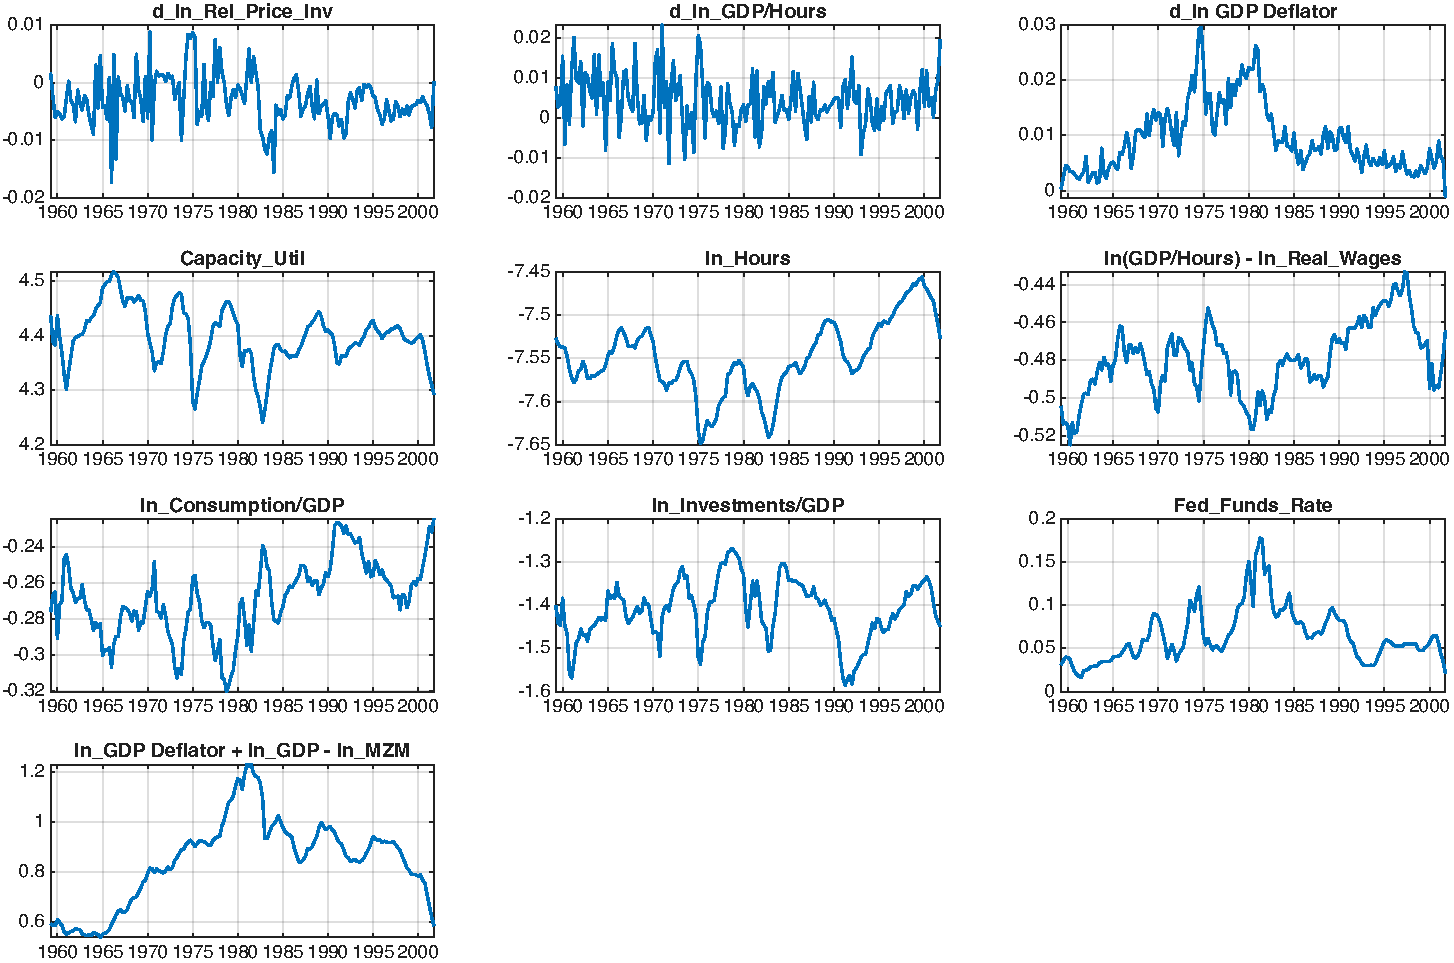
\includegraphics[width=1\linewidth]{../../Output/Descriptive_Statistics/Raw_Historical_Series.pdf}}{\fbox{Image Path Broken or File Missing}}
    \caption{Raw Historical Series}
    \label{fig:raw_series}
\end{figure}
\FloatBarrier

\clearpage
\subsection{ACEL 2005 VAR Across different lag structures: Monetary Policy Shock}

\begin{figure}[htpb]
    \centering
    \IfFileExists{../../Output/LDC_ACEL2011_Impulse_Response_Matching/MP/MP_lag_4.pdf}
    {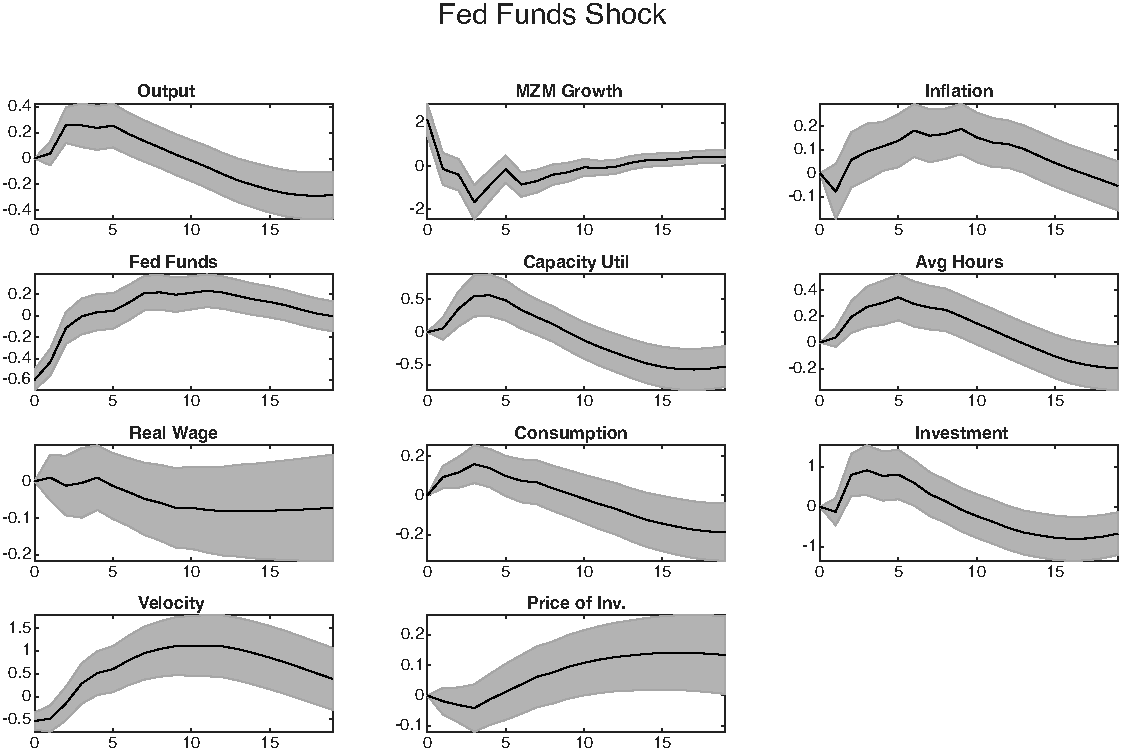
\includegraphics[width=1\linewidth]{../../Output/LDC_ACEL2011_Impulse_Response_Matching/MP/MP_lag_4.pdf}}{\fbox{Image Path Broken or File Missing}}
    \caption{Monetary Policy Shock lag 4}
    \label{fig:mp_baseline_lag4}
\end{figure}

\begin{figure}[htpb]
    \centering
    \IfFileExists{../../Output/LDC_ACEL2011_Impulse_Response_Matching/MP/MP_lag_6.pdf}
    {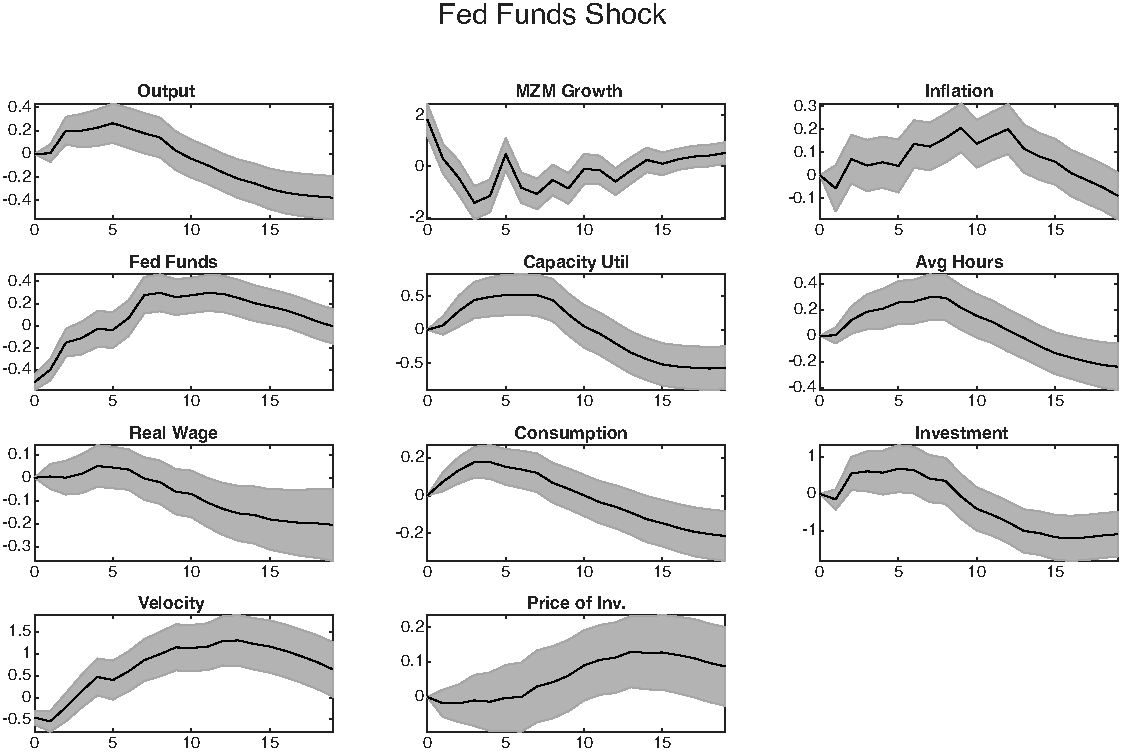
\includegraphics[width=1\linewidth]{../../Output/LDC_ACEL2011_Impulse_Response_Matching/MP/MP_lag_6.pdf}}{\fbox{Image Path Broken or File Missing}}
    \caption{Monetary Policy Shock lag 6}
    \label{fig:mp_baseline_lag6}
\end{figure}

\begin{figure}[htpb]
    \centering
    \IfFileExists{../../Output/LDC_ACEL2011_Impulse_Response_Matching/MP/MP_lag_8.pdf}
    {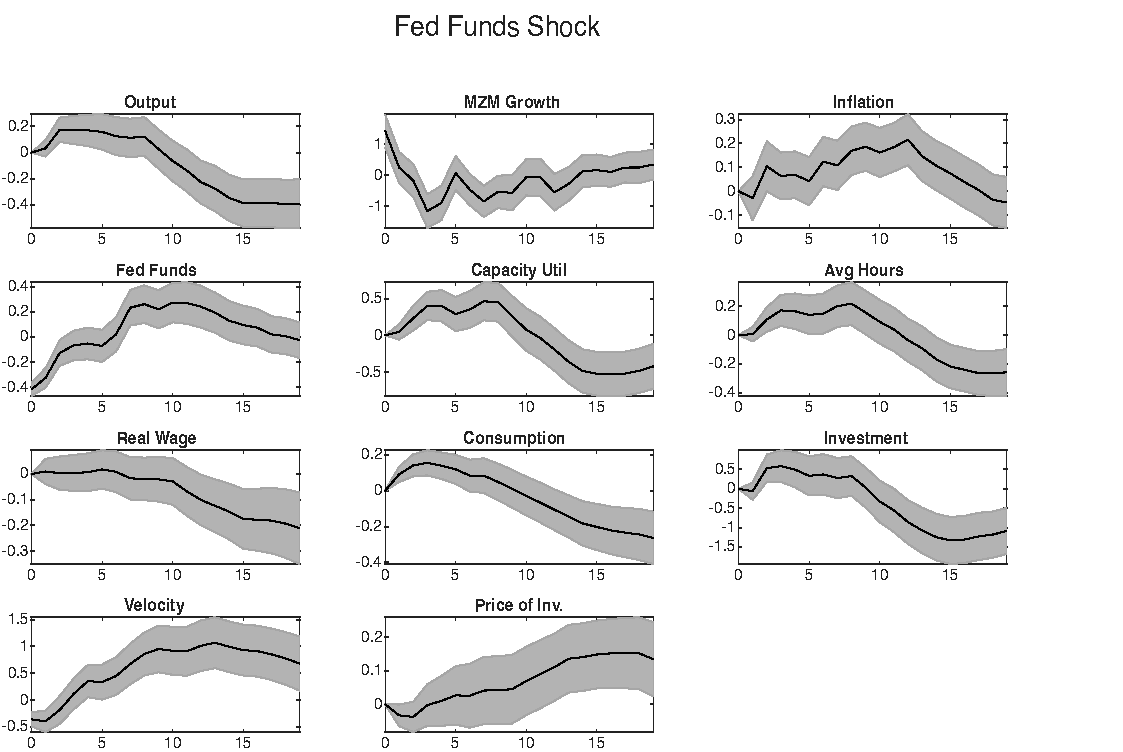
\includegraphics[width=1\linewidth]{../../Output/LDC_ACEL2011_Impulse_Response_Matching/MP/MP_lag_8.pdf}}{\fbox{Image Path Broken or File Missing}}
    \caption{Monetary Policy Shock lag 8}
    \label{fig:mp_baseline_lag8}
\end{figure}

\begin{figure}[htpb]
    \centering
    \IfFileExists{../../Output/LDC_ACEL2011_Impulse_Response_Matching/MP/MP_lag_10.pdf}
    {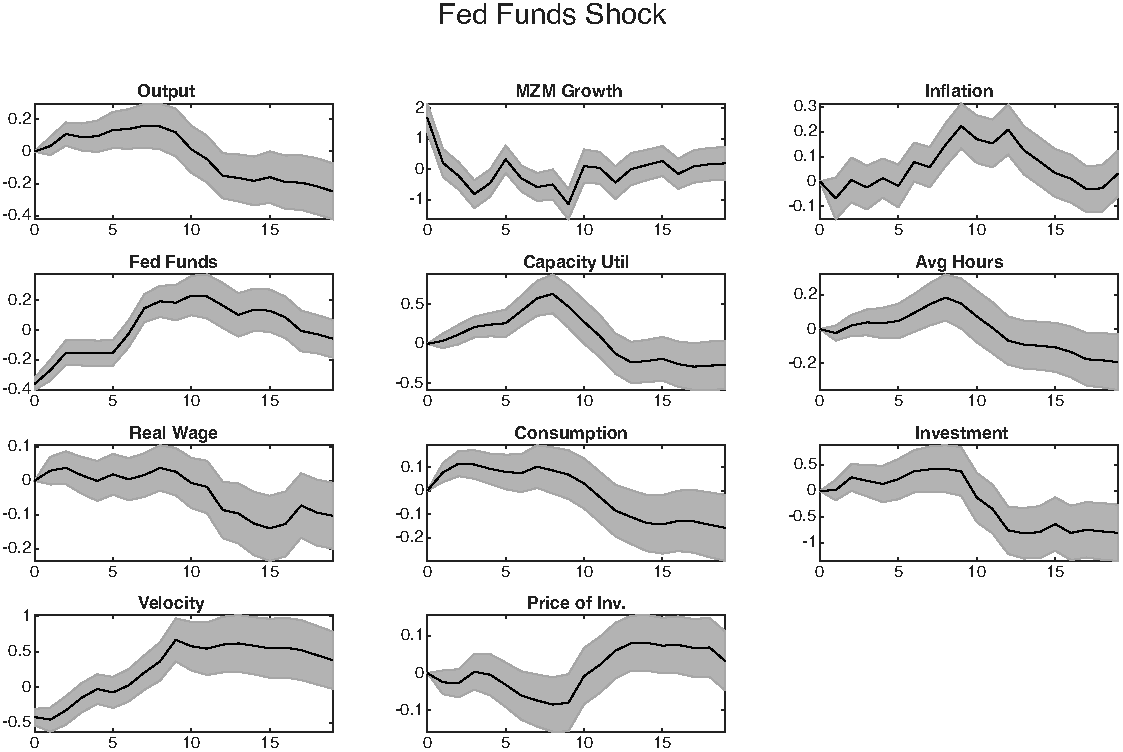
\includegraphics[width=1\linewidth]{../../Output/LDC_ACEL2011_Impulse_Response_Matching/MP/MP_lag_10.pdf}}{\fbox{Image Path Broken or File Missing}}
    \caption{Monetary Policy Shock lag 10}
    \label{fig:mp_baseline_lag10}
\end{figure}

\begin{figure}[htpb]
    \centering
    \IfFileExists{../../Output/LDC_ACEL2011_Impulse_Response_Matching/MP/MP_lag_12.pdf}
    {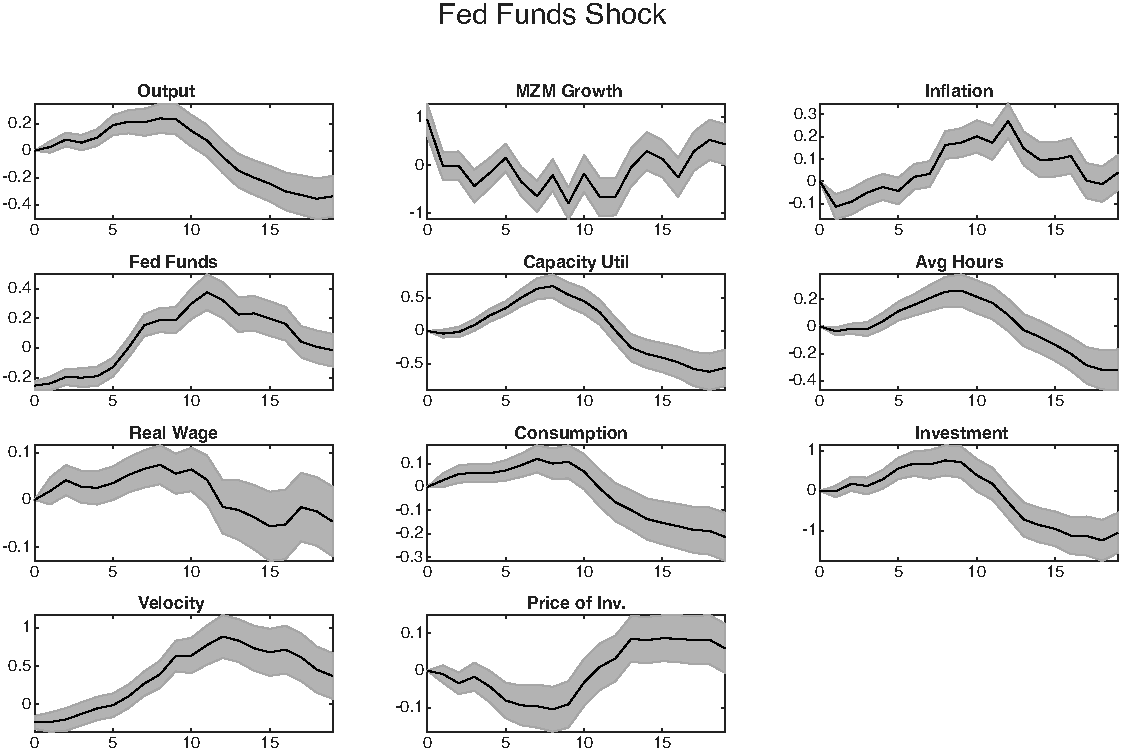
\includegraphics[width=1\linewidth]{../../Output/LDC_ACEL2011_Impulse_Response_Matching/MP/MP_lag_12.pdf}}{\fbox{Image Path Broken or File Missing}}
    \caption{Monetary Policy Shock lag 12}
    \label{fig:mp_baseline_lag12}
\end{figure}

\FloatBarrier

\clearpage
\subsection{ACEL 2005 VAR Across different lag structures: Embodied Technology Shock}

\begin{figure}[htpb]
    \centering
    \IfFileExists{../../Output/LDC_ACEL2011_Impulse_Response_Matching/ET/ET_lag_4.pdf}
    {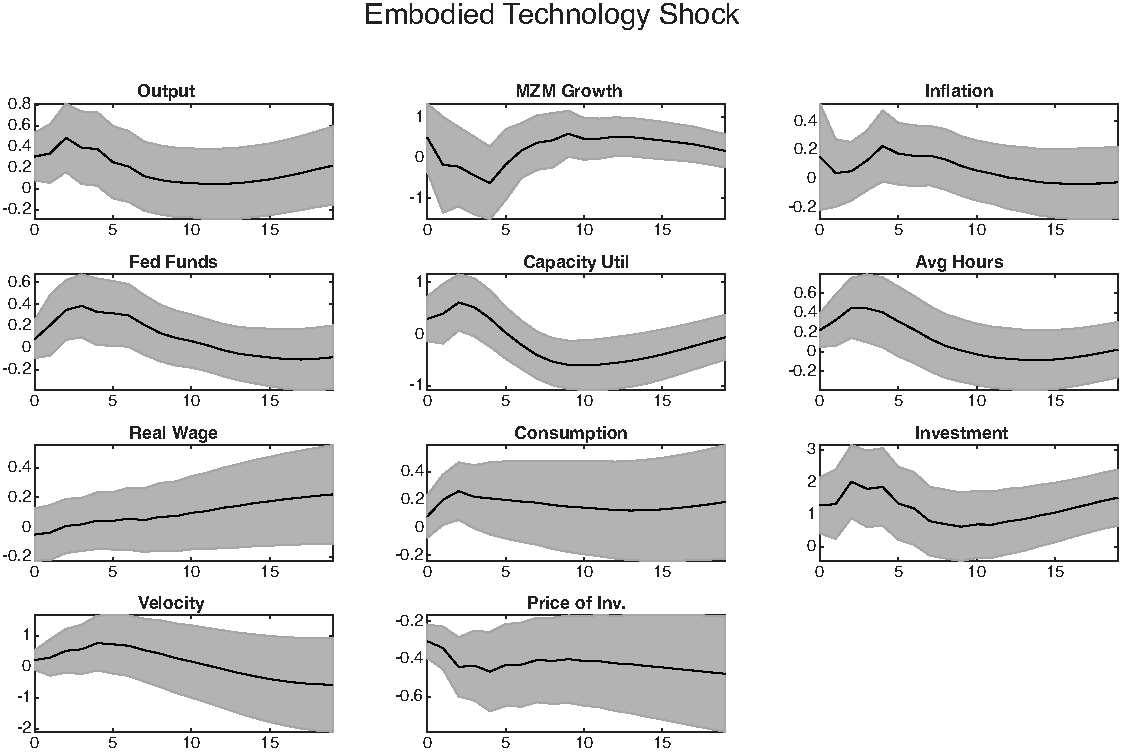
\includegraphics[width=1\linewidth]{../../Output/LDC_ACEL2011_Impulse_Response_Matching/ET/ET_lag_4.pdf}}{\fbox{Image Path Broken or File Missing}}
    \caption{Embodied Technology Shock lag 4}
    \label{fig:et_baseline_lag4}
\end{figure}

\begin{figure}[htpb]
    \centering
    \IfFileExists{../../Output/LDC_ACEL2011_Impulse_Response_Matching/ET/ET_lag_6.pdf}
    {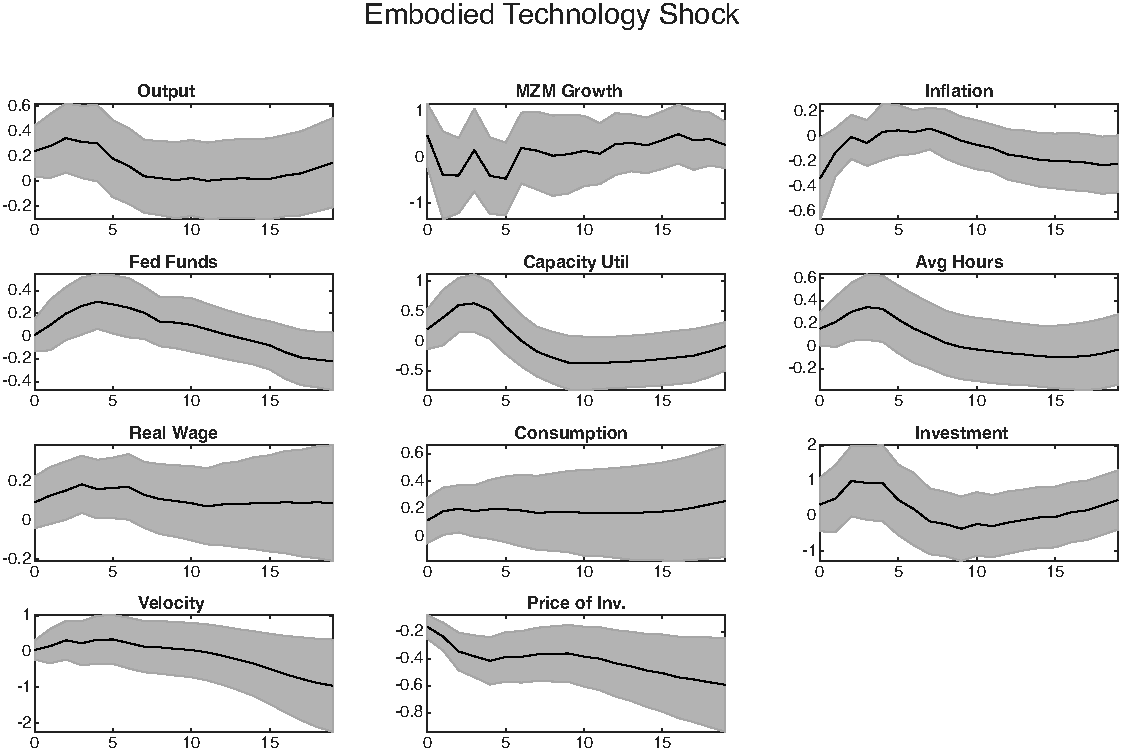
\includegraphics[width=1\linewidth]{../../Output/LDC_ACEL2011_Impulse_Response_Matching/ET/ET_lag_6.pdf}}{\fbox{Image Path Broken or File Missing}}
    \caption{Embodied Technology Shock lag 6}
    \label{fig:et_baseline_lag6}
\end{figure}

\begin{figure}[htpb]
    \centering
    \IfFileExists{../../Output/LDC_ACEL2011_Impulse_Response_Matching/ET/ET_lag_8.pdf}
    {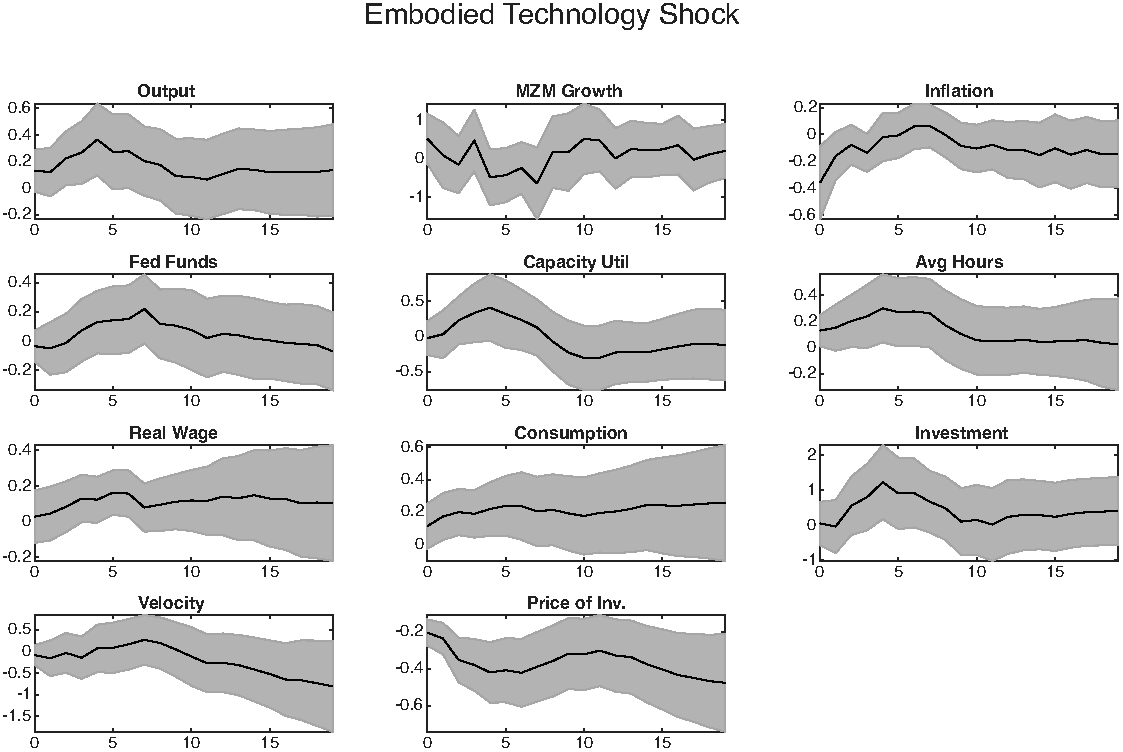
\includegraphics[width=1\linewidth]{../../Output/LDC_ACEL2011_Impulse_Response_Matching/ET/ET_lag_8.pdf}}{\fbox{Image Path Broken or File Missing}}
    \caption{Embodied Technology Shock lag 8}
    \label{fig:et_baseline_lag8}
\end{figure}

\begin{figure}[htpb]
    \centering
    \IfFileExists{../../Output/LDC_ACEL2011_Impulse_Response_Matching/ET/ET_lag_10.pdf}
    {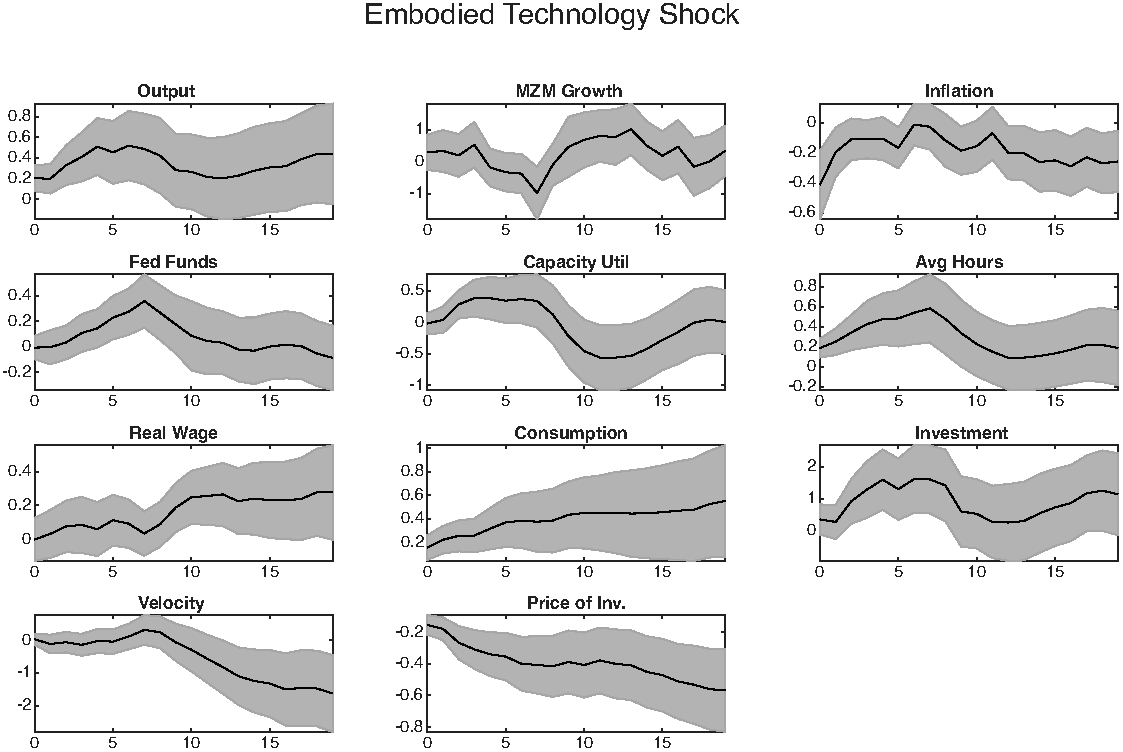
\includegraphics[width=1\linewidth]{../../Output/LDC_ACEL2011_Impulse_Response_Matching/ET/ET_lag_10.pdf}}{\fbox{Image Path Broken or File Missing}}
    \caption{Embodied Technology Shock lag 10}
    \label{fig:et_baseline_lag10}
\end{figure}

\begin{figure}[htpb]
    \centering
    \IfFileExists{../../Output/LDC_ACEL2011_Impulse_Response_Matching/ET/ET_lag_12.pdf}
    {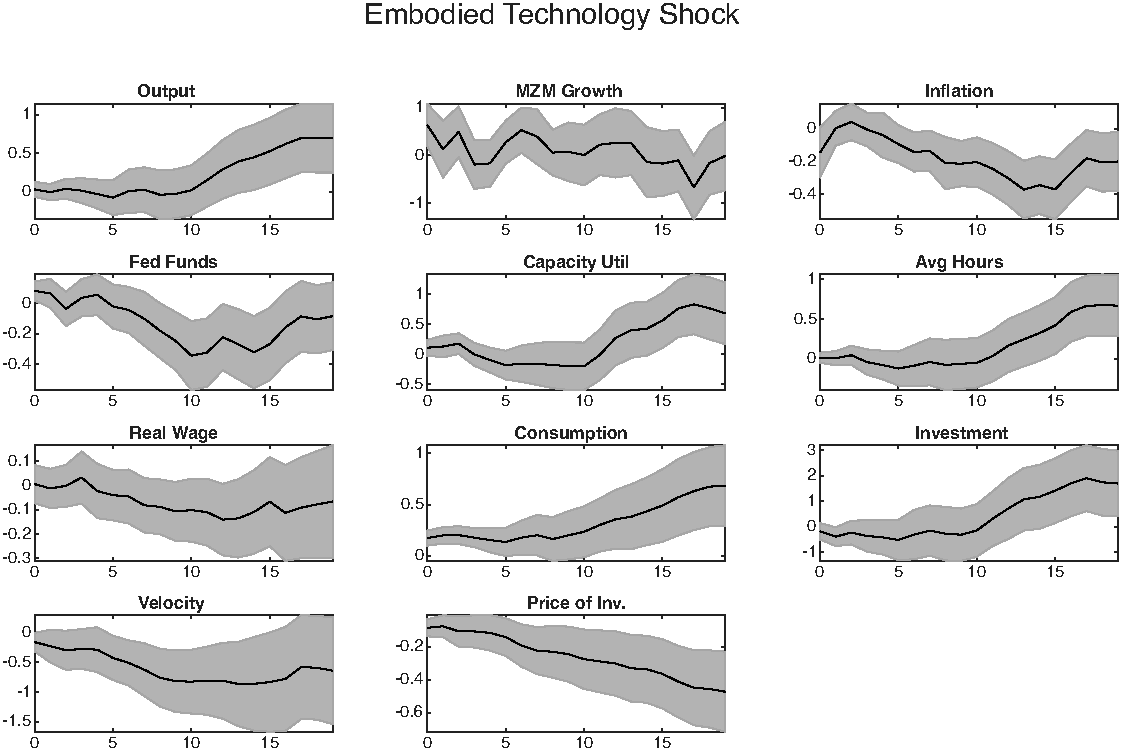
\includegraphics[width=1\linewidth]{../../Output/LDC_ACEL2011_Impulse_Response_Matching/ET/ET_lag_12.pdf}}{\fbox{Image Path Broken or File Missing}}
    \caption{Embodied Technology Shock lag 12}
    \label{fig:et_baseline_lag12}
\end{figure}

\FloatBarrier

\clearpage
\subsection{ACEL 2005 VAR Across different lag structures: Neutral Technology Shock}

\begin{figure}[htpb]
    \centering
    \IfFileExists{../../Output/LDC_ACEL2011_Impulse_Response_Matching/NT/NT_lag_4.pdf}
    {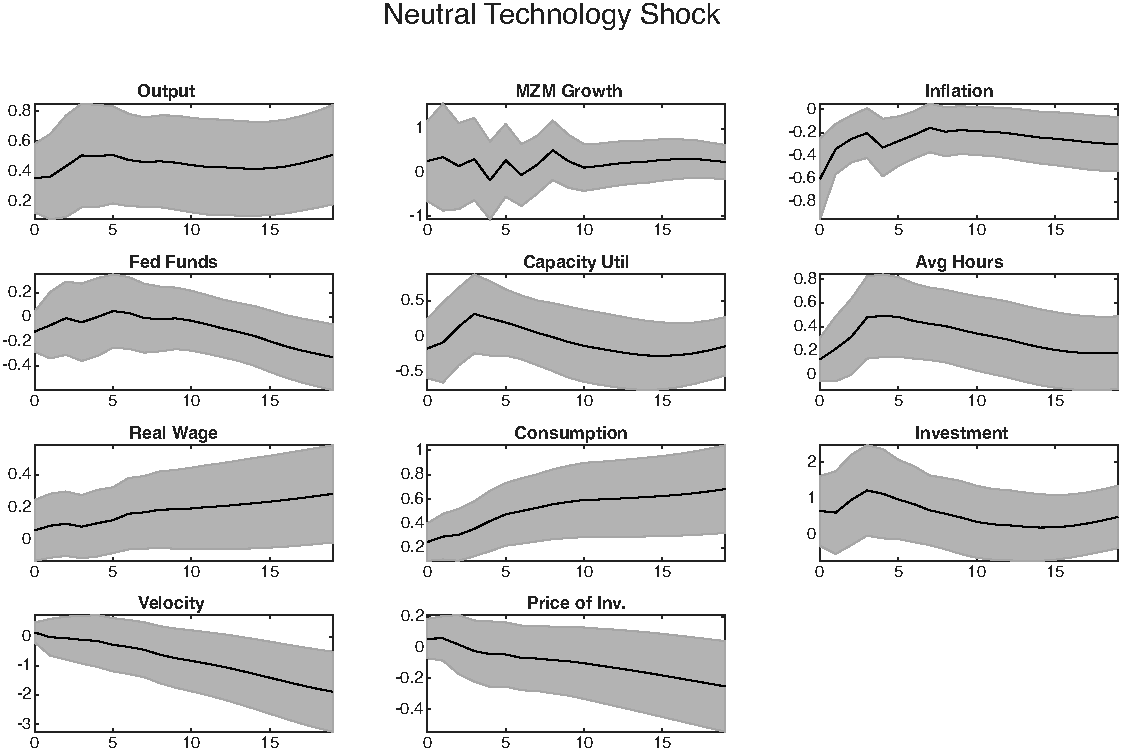
\includegraphics[width=1\linewidth]{../../Output/LDC_ACEL2011_Impulse_Response_Matching/NT/NT_lag_4.pdf}}{\fbox{Image Path Broken or File Missing}}
    \caption{Neutral Technology Shock lag 4}
    \label{fig:nt_baseline_lag4}
\end{figure}

\begin{figure}[htpb]
    \centering
    \IfFileExists{../../Output/LDC_ACEL2011_Impulse_Response_Matching/NT/NT_lag_6.pdf}
    {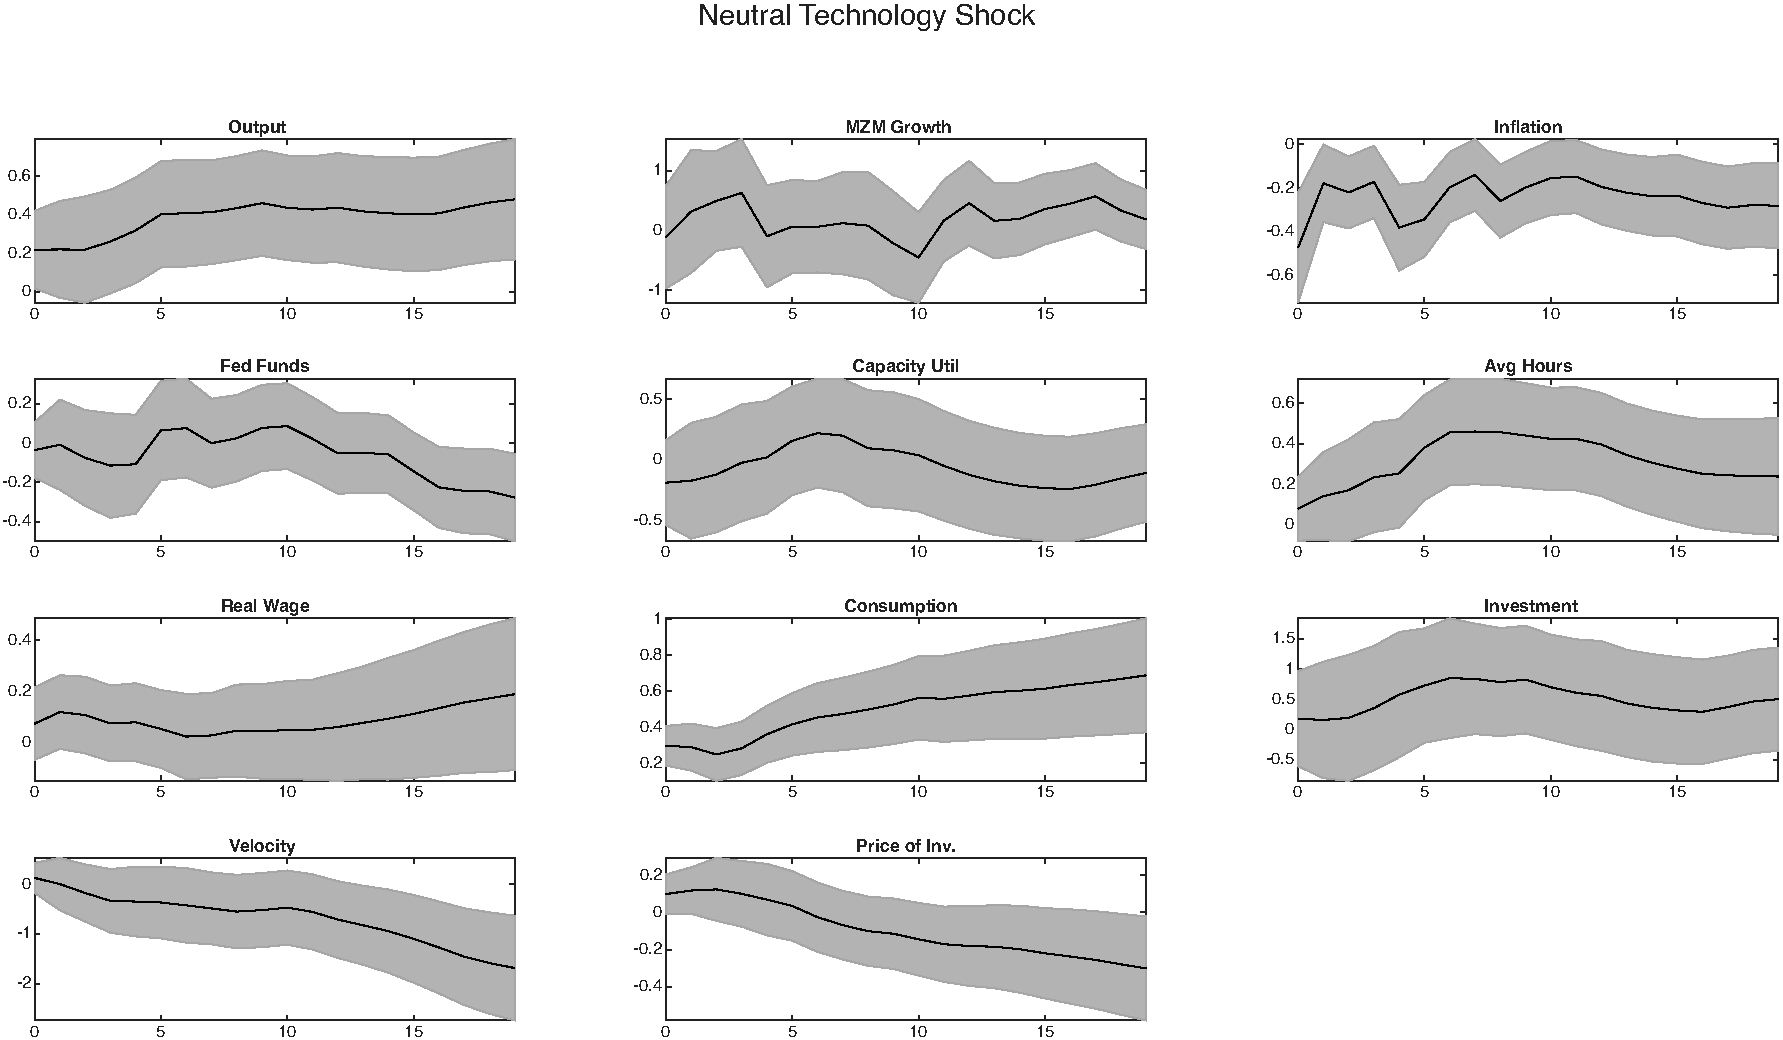
\includegraphics[width=1\linewidth]{../../Output/LDC_ACEL2011_Impulse_Response_Matching/NT/NT_lag_6.pdf}}{\fbox{Image Path Broken or File Missing}}
    \caption{Neutral Technology Shock lag 6}
    \label{fig:nt_baseline_lag6}
\end{figure}

\begin{figure}[htpb]
    \centering
    \IfFileExists{../../Output/LDC_ACEL2011_Impulse_Response_Matching/NT/NT_lag_8.pdf}
    {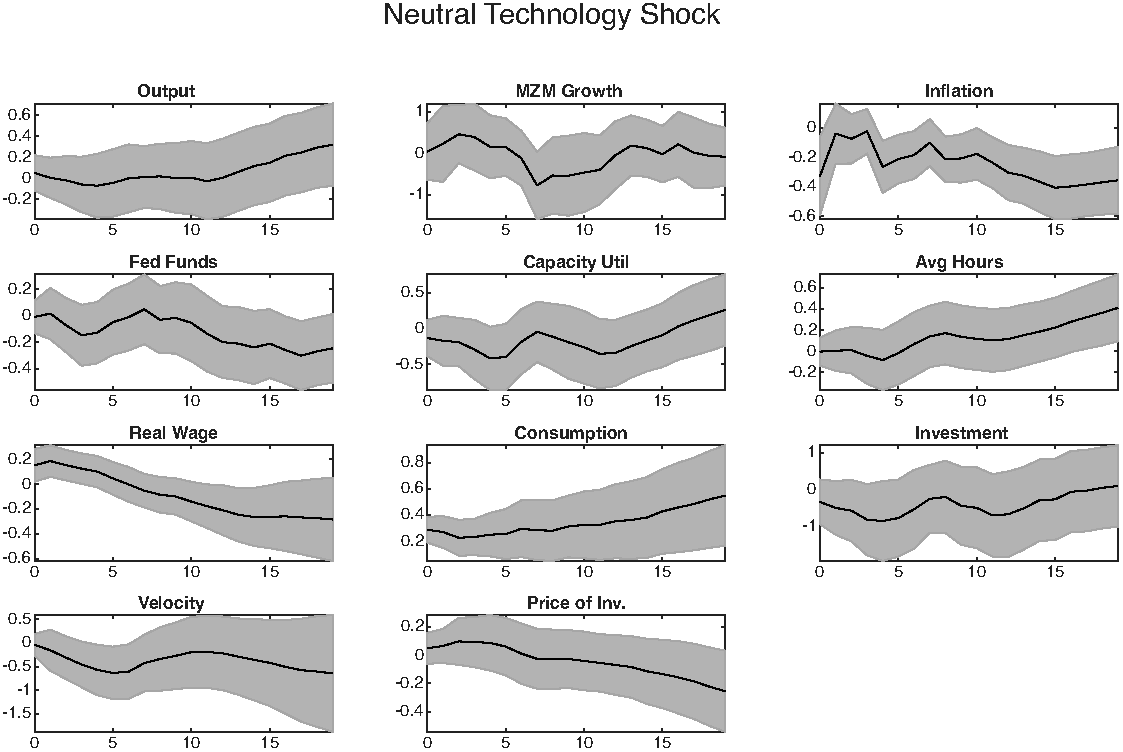
\includegraphics[width=1\linewidth]{../../Output/LDC_ACEL2011_Impulse_Response_Matching/NT/NT_lag_8.pdf}}{\fbox{Image Path Broken or File Missing}}
    \caption{Neutral Technology Shock lag 8}
    \label{fig:nt_baseline_lag8}
\end{figure}

\begin{figure}[htpb]
    \centering
    \IfFileExists{../../Output/LDC_ACEL2011_Impulse_Response_Matching/NT/NT_lag_10.pdf}
    {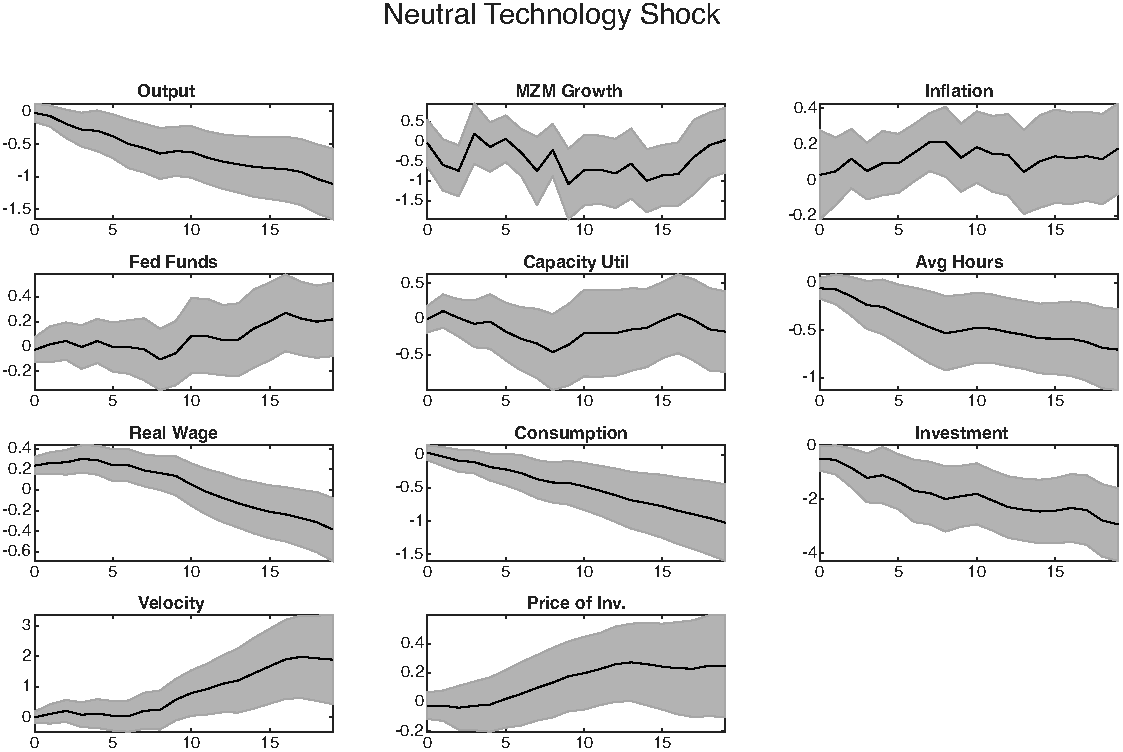
\includegraphics[width=1\linewidth]{../../Output/LDC_ACEL2011_Impulse_Response_Matching/NT/NT_lag_10.pdf}}{\fbox{Image Path Broken or File Missing}}
    \caption{Neutral Technology Shock lag 10}
    \label{fig:nt_baseline_lag10}
\end{figure}

\begin{figure}[htpb]
    \centering
    \IfFileExists{../../Output/LDC_ACEL2011_Impulse_Response_Matching/NT/NT_lag_12.pdf}
    {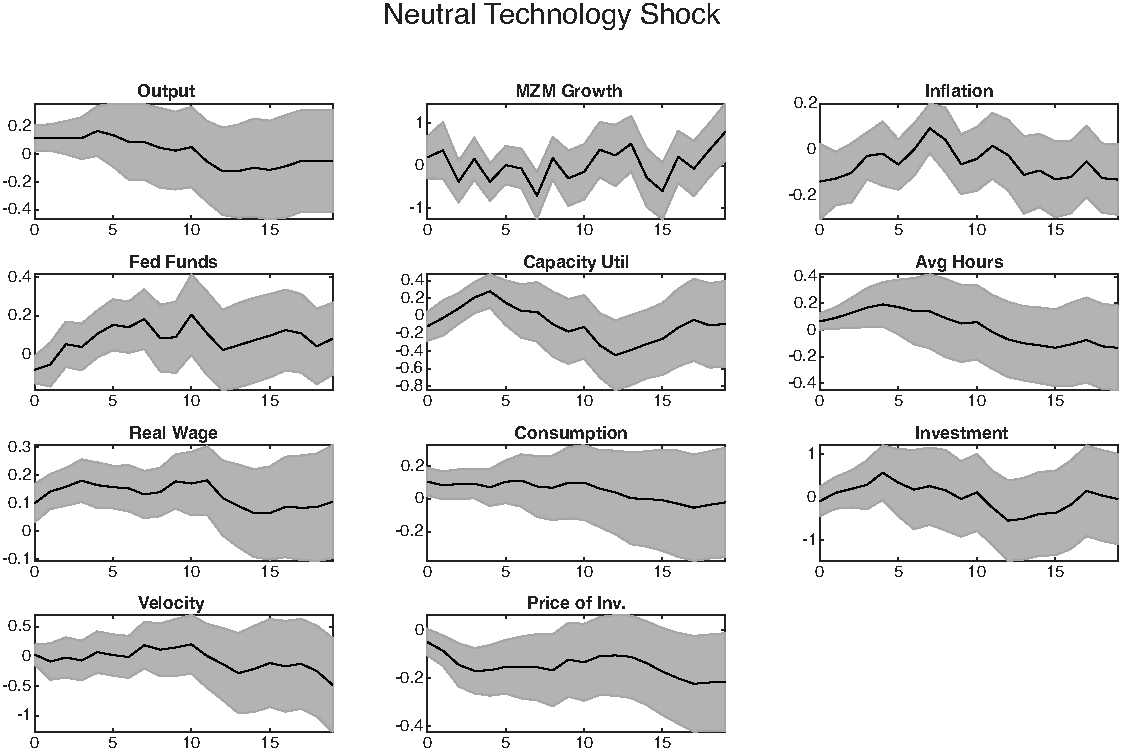
\includegraphics[width=1\linewidth]{../../Output/LDC_ACEL2011_Impulse_Response_Matching/NT/NT_lag_12.pdf}}{\fbox{Image Path Broken or File Missing}}
    \caption{Neutral Technology Shock lag 12}
    \label{fig:nt_baseline_lag12}
\end{figure}

\FloatBarrier

\clearpage

\subsection{ACEL 2005 DSGE Matched with VAR 4, compared with VAR estimated across different lag structures: Monetary Policy Shock}

\begin{figure}[htpb]
    \centering
    \IfFileExists{../../Output/LDC_ACEL2011_Impulse_Response_Matching/MP_basic_DSGE/MP_DSGE4_lag_4.pdf}
        {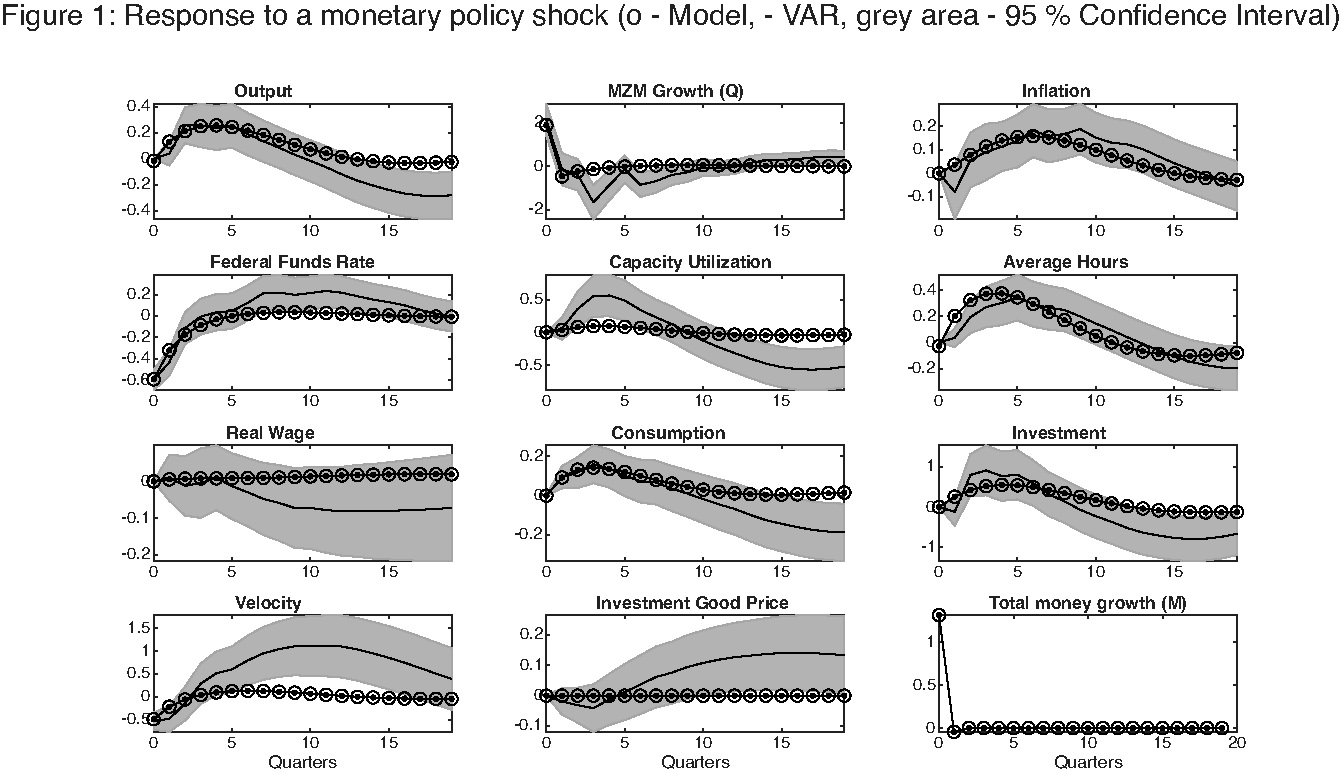
\includegraphics[width=1\linewidth]{../../Output/LDC_ACEL2011_Impulse_Response_Matching/MP_basic_DSGE/MP_DSGE4_lag_4.pdf}}
        {\fbox{Image Path Broken or File Missing}}
    \caption{Monetary Policy Shock DSGE matched with VAR lag 4 compared to VAR lag 4}
    \label{fig:basic_mp_lag4}
\end{figure}

\begin{figure}[htpb]
    \centering
    \IfFileExists{../../Output/LDC_ACEL2011_Impulse_Response_Matching/MP_basic_DSGE/MP_DSGE4_lag_6.pdf}
        {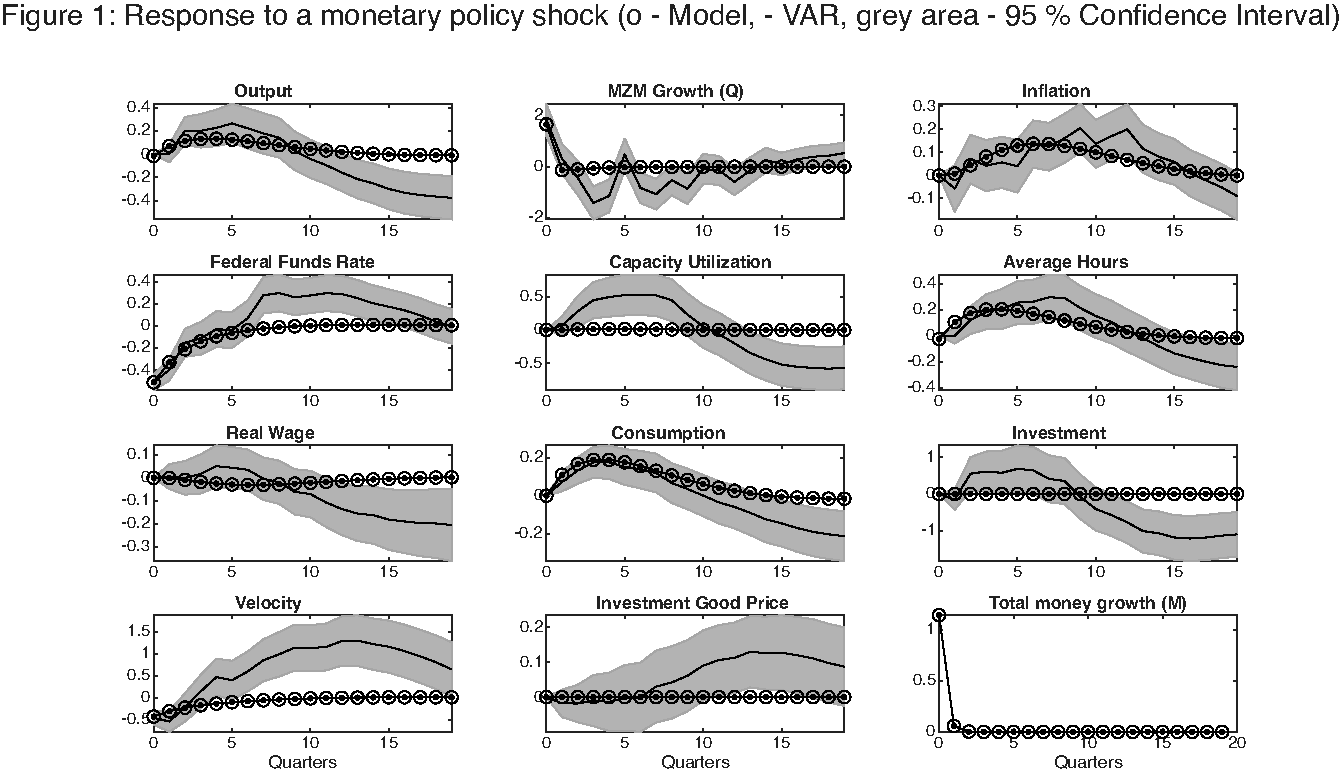
\includegraphics[width=1\linewidth]{../../Output/LDC_ACEL2011_Impulse_Response_Matching/MP_basic_DSGE/MP_DSGE4_lag_6.pdf}}
        {\fbox{Image Path Broken or File Missing}}
    \caption{Monetary Policy Shock DSGE matched with VAR lag 4 compared to VAR lag 6}
    \label{fig:basic_mp_lag6}
\end{figure}

\begin{figure}[htpb]
    \centering
    \IfFileExists{../../Output/LDC_ACEL2011_Impulse_Response_Matching/MP_basic_DSGE/MP_DSGE4_lag_8.pdf}
        {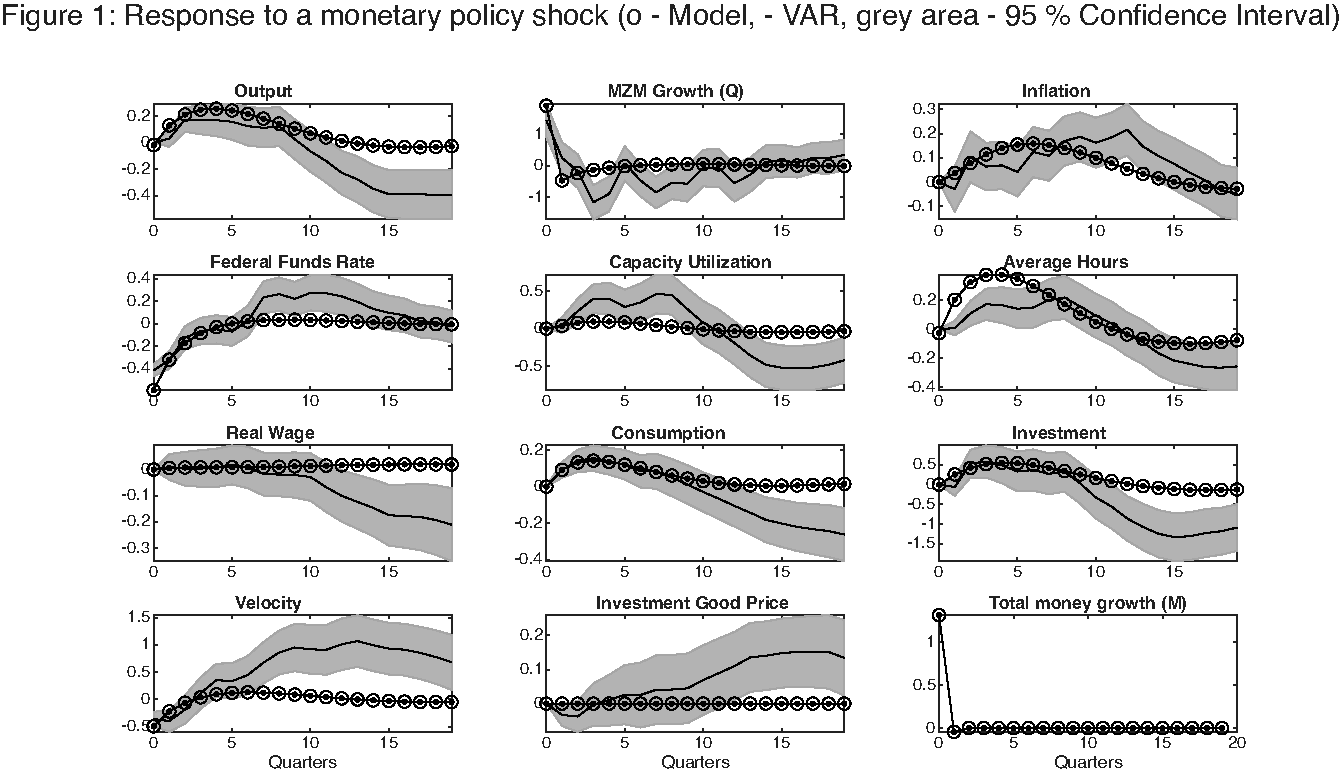
\includegraphics[width=1\linewidth]{../../Output/LDC_ACEL2011_Impulse_Response_Matching/MP_basic_DSGE/MP_DSGE4_lag_8.pdf}}
        {\fbox{Image Path Broken or File Missing}}
    \caption{Monetary Policy Shock DSGE matched with VAR lag 4 compared to VAR lag 8}
    \label{fig:basic_mp_lag8}
\end{figure}

\begin{figure}[htpb]
    \centering
    \IfFileExists{../../Output/LDC_ACEL2011_Impulse_Response_Matching/MP_basic_DSGE/MP_DSGE4_lag_10.pdf}
        {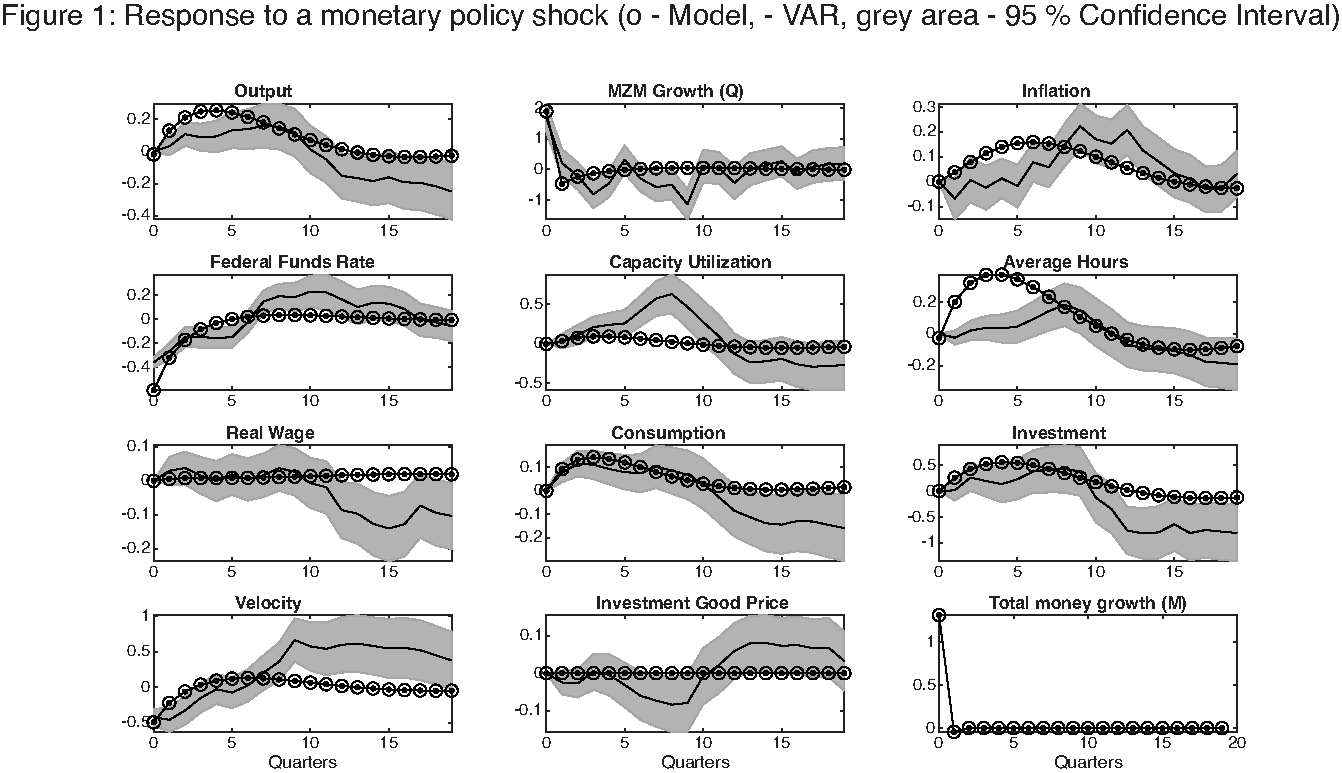
\includegraphics[width=1\linewidth]{../../Output/LDC_ACEL2011_Impulse_Response_Matching/MP_basic_DSGE/MP_DSGE4_lag_10.pdf}}
        {\fbox{Image Path Broken or File Missing}}
    \caption{Monetary Policy Shock DSGE matched with VAR lag 4 compared to VAR lag 10}
    \label{fig:basic_mp_lag10}
\end{figure}

\begin{figure}[htpb]
    \centering
    \IfFileExists{../../Output/LDC_ACEL2011_Impulse_Response_Matching/MP_basic_DSGE/MP_DSGE4_lag_12.pdf}
        {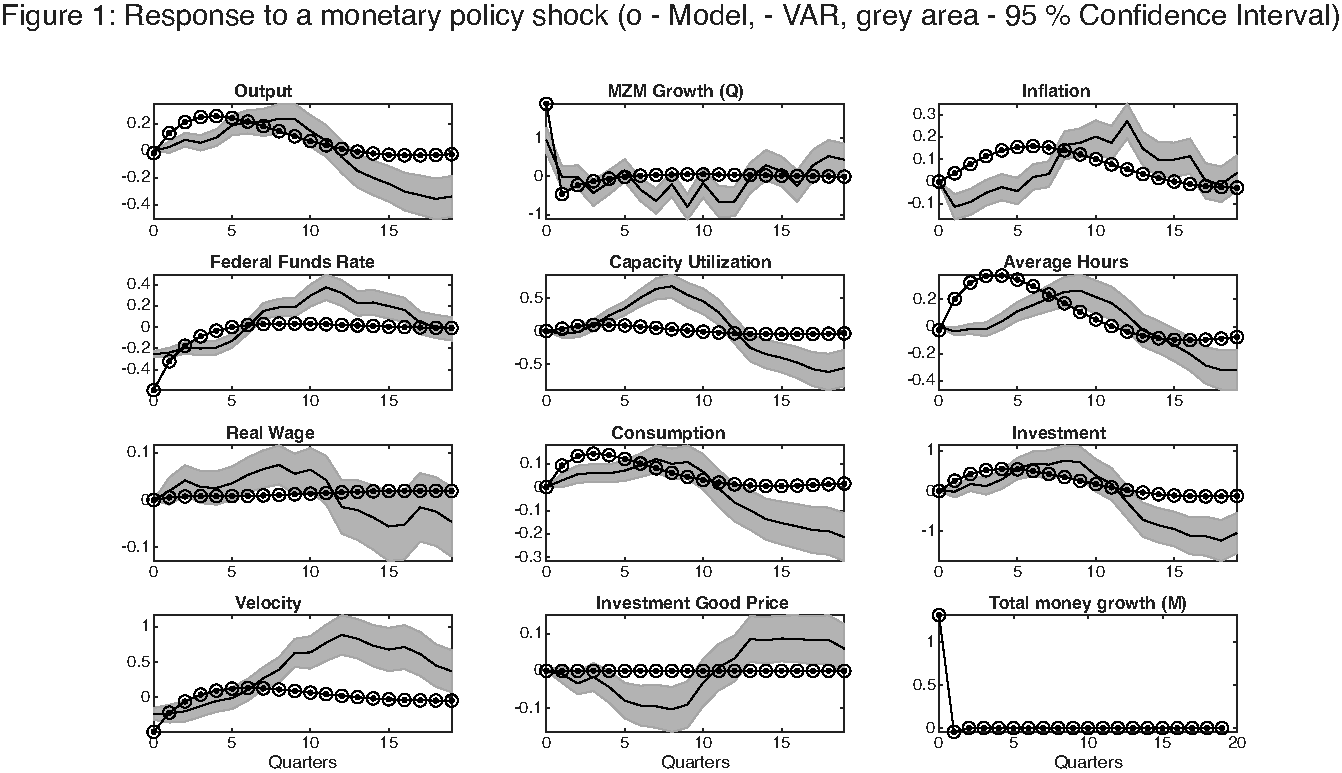
\includegraphics[width=1\linewidth]{../../Output/LDC_ACEL2011_Impulse_Response_Matching/MP_basic_DSGE/MP_DSGE4_lag_12.pdf}}
        {\fbox{Image Path Broken or File Missing}}
    \caption{Monetary Policy Shock DSGE matched with VAR lag 4 compared to VAR lag 12}
    \label{fig:basic_mp_lag12}
\end{figure}

\FloatBarrier

\clearpage
\subsection{ACEL 2005 DSGE Matched with VAR 4, compared with VAR estimated across different lag structures: Embodied Technology Shock}

\begin{figure}[htpb]
    \centering
    \IfFileExists{../../Output/LDC_ACEL2011_Impulse_Response_Matching/ET_basic_DSGE/ET_DSGE4_lag_4.pdf}
        {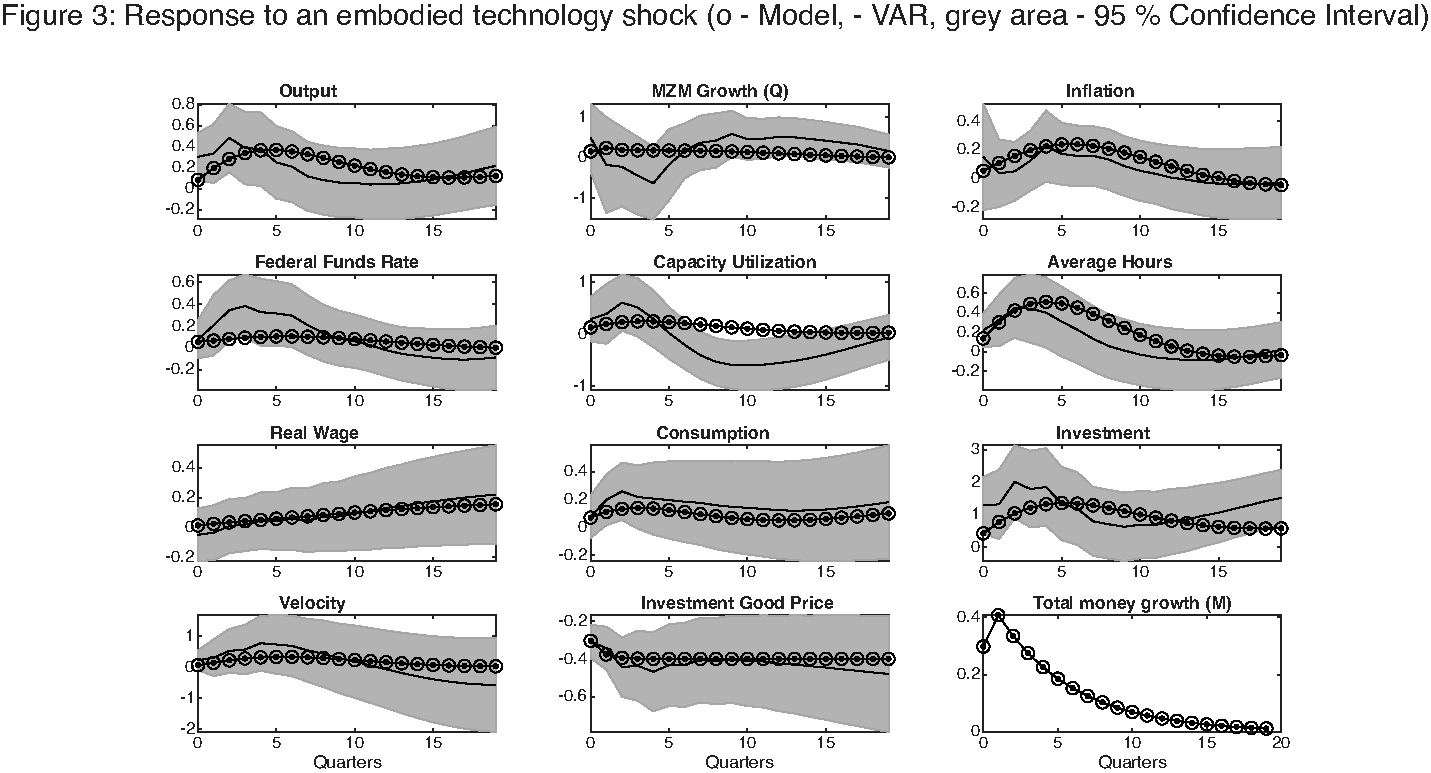
\includegraphics[width=1\linewidth]{../../Output/LDC_ACEL2011_Impulse_Response_Matching/ET_basic_DSGE/ET_DSGE4_lag_4.pdf}}
        {\fbox{Image Path Broken or File Missing}}
    \caption{Embodied Technology Shock DSGE matched with VAR lag 4 compared to VAR lag 4}
    \label{fig:basic_et_lag4}
\end{figure}

\begin{figure}[htpb]
    \centering
    \IfFileExists{../../Output/LDC_ACEL2011_Impulse_Response_Matching/ET_basic_DSGE/ET_DSGE4_lag_6.pdf}
        {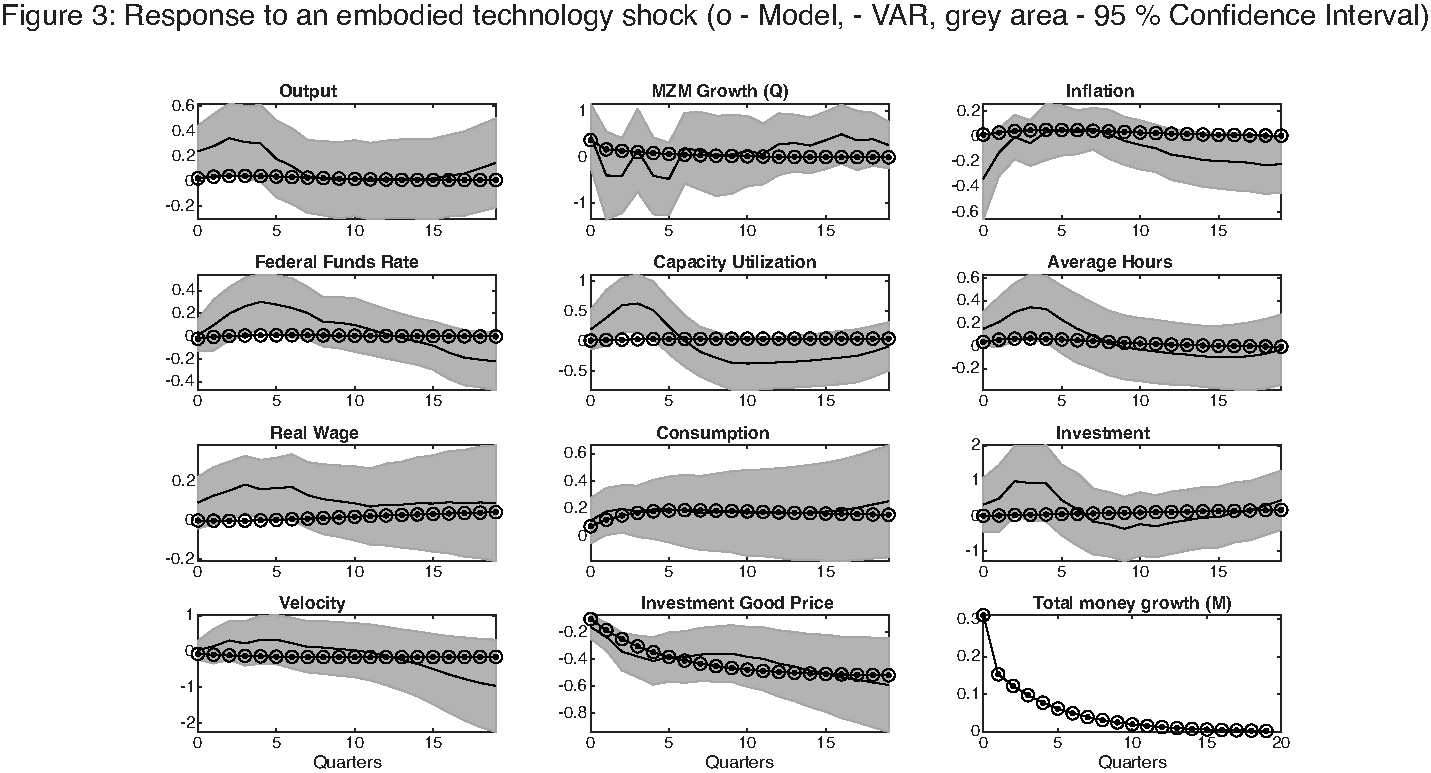
\includegraphics[width=1\linewidth]{../../Output/LDC_ACEL2011_Impulse_Response_Matching/ET_basic_DSGE/ET_DSGE4_lag_6.pdf}}
        {\fbox{Image Path Broken or File Missing}}
    \caption{Embodied Technology Shock DSGE matched with VAR lag 4 compared to VAR lag 6}
    \label{fig:basic_et_lag6}
\end{figure}

\begin{figure}[htpb]
    \centering
    \IfFileExists{../../Output/LDC_ACEL2011_Impulse_Response_Matching/ET_basic_DSGE/ET_DSGE4_lag_8.pdf}
        {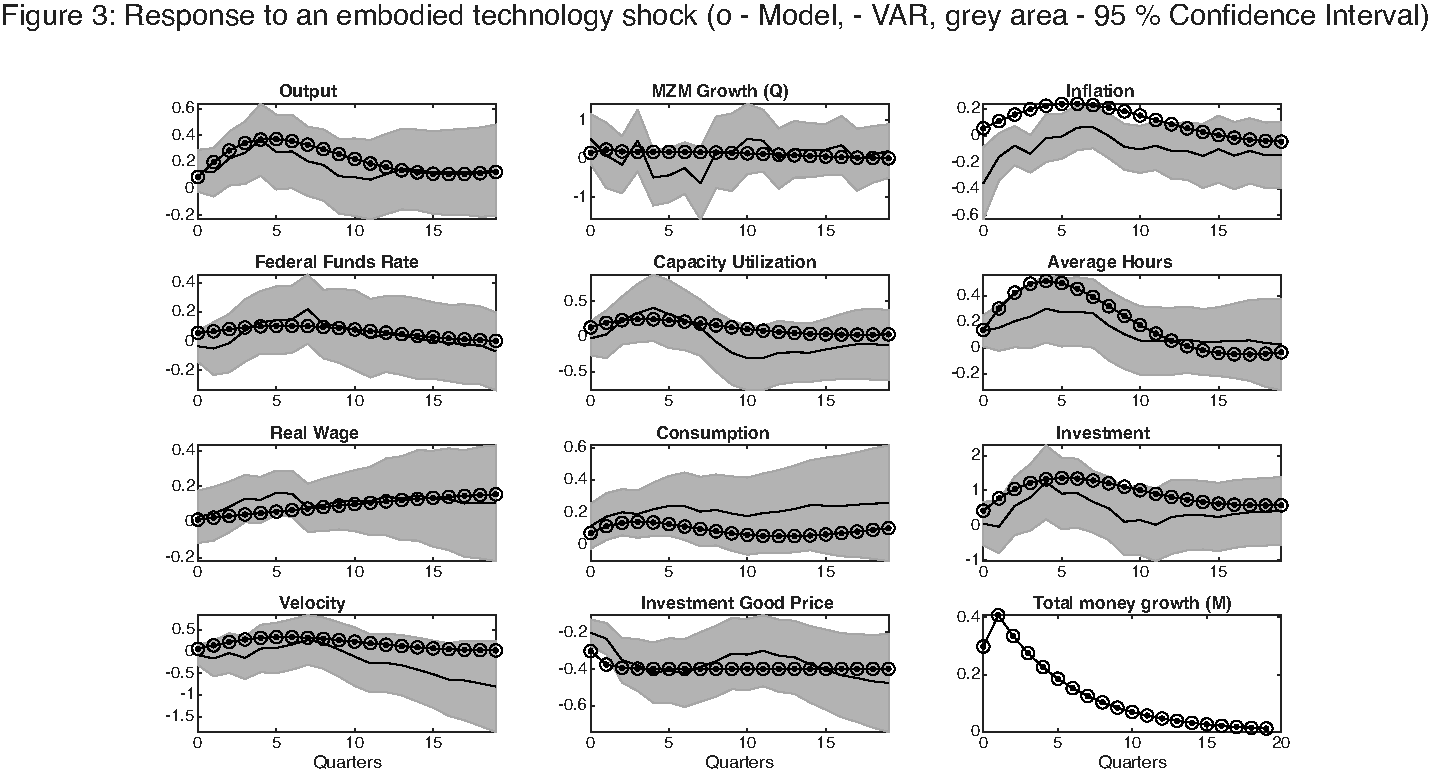
\includegraphics[width=1\linewidth]{../../Output/LDC_ACEL2011_Impulse_Response_Matching/ET_basic_DSGE/ET_DSGE4_lag_8.pdf}}
        {\fbox{Image Path Broken or File Missing}}
    \caption{Embodied Technology Shock DSGE matched with VAR lag 4 compared to VAR lag 8}
    \label{fig:basic_et_lag8}
\end{figure}

\begin{figure}[htpb]
    \centering
    \IfFileExists{../../Output/LDC_ACEL2011_Impulse_Response_Matching/ET_basic_DSGE/ET_DSGE4_lag_10.pdf}
        {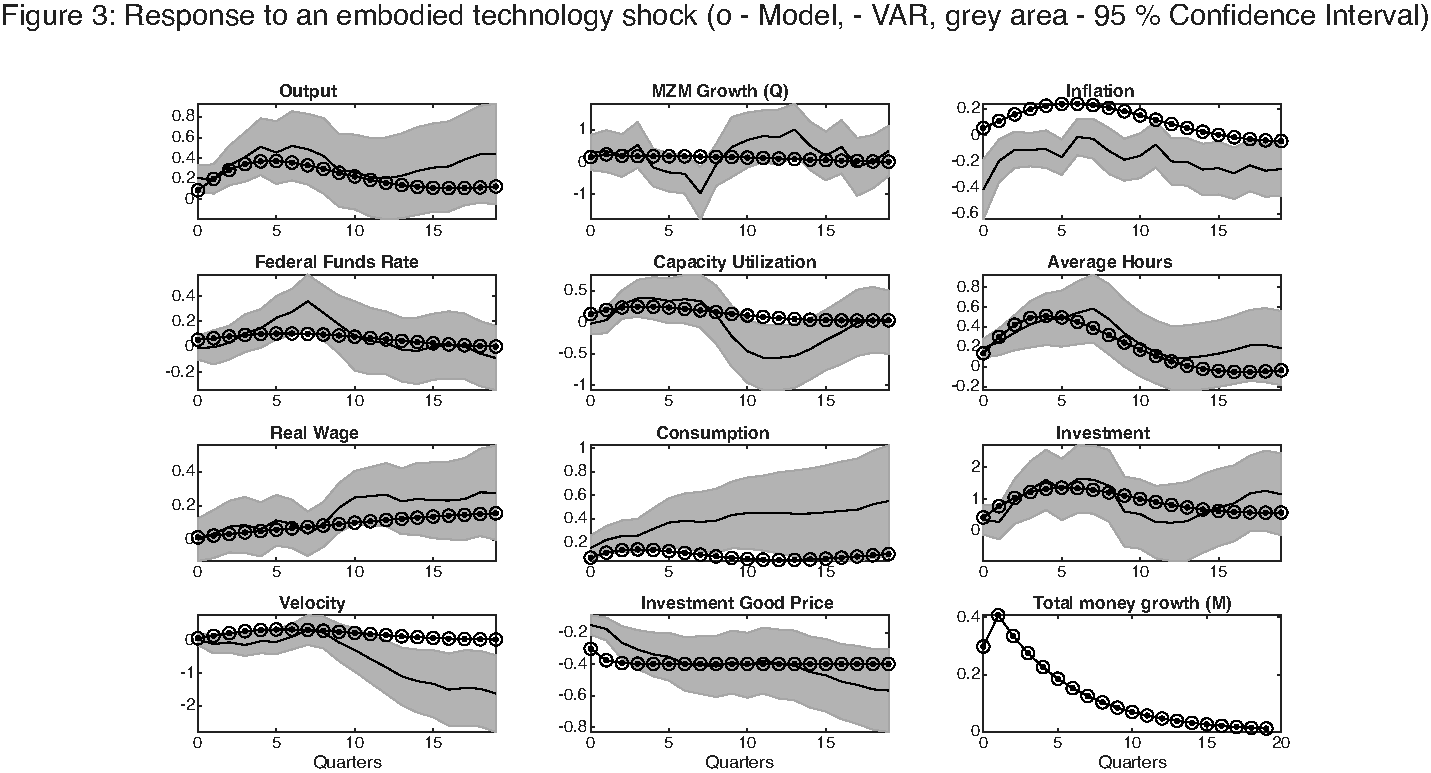
\includegraphics[width=1\linewidth]{../../Output/LDC_ACEL2011_Impulse_Response_Matching/ET_basic_DSGE/ET_DSGE4_lag_10.pdf}}
        {\fbox{Image Path Broken or File Missing}}
    \caption{Embodied Technology Shock DSGE matched with VAR lag 4 compared to VAR lag 10}
    \label{fig:basic_et_lag10}
\end{figure}

\begin{figure}[htpb]
    \centering
    \IfFileExists{../../Output/LDC_ACEL2011_Impulse_Response_Matching/ET_basic_DSGE/ET_DSGE4_lag_12.pdf}
        {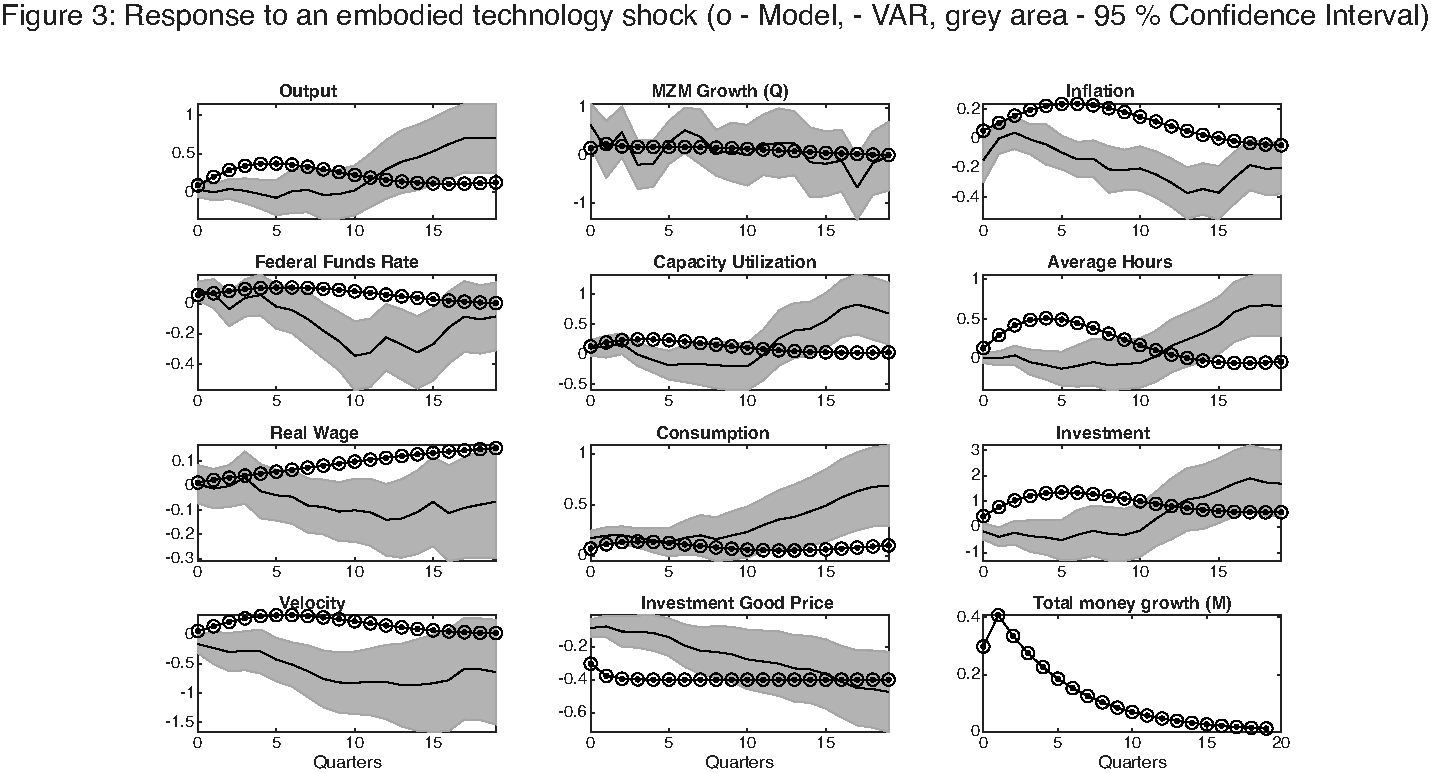
\includegraphics[width=1\linewidth]{../../Output/LDC_ACEL2011_Impulse_Response_Matching/ET_basic_DSGE/ET_DSGE4_lag_12.pdf}}
        {\fbox{Image Path Broken or File Missing}}
    \caption{Embodied Technology Shock DSGE matched with VAR lag 4 compared to VAR lag 12}
    \label{fig:basic_et_lag12}
\end{figure}

\FloatBarrier

\clearpage
\subsection{ACEL 2005 DSGE Matched with VAR 4, compared with VAR estimated across different lag structures: Neutral Technology Shock}

\begin{figure}[htpb]
    \centering
    \IfFileExists{../../Output/LDC_ACEL2011_Impulse_Response_Matching/NT_basic_DSGE/NT_DSGE4_lag_4.pdf}
        {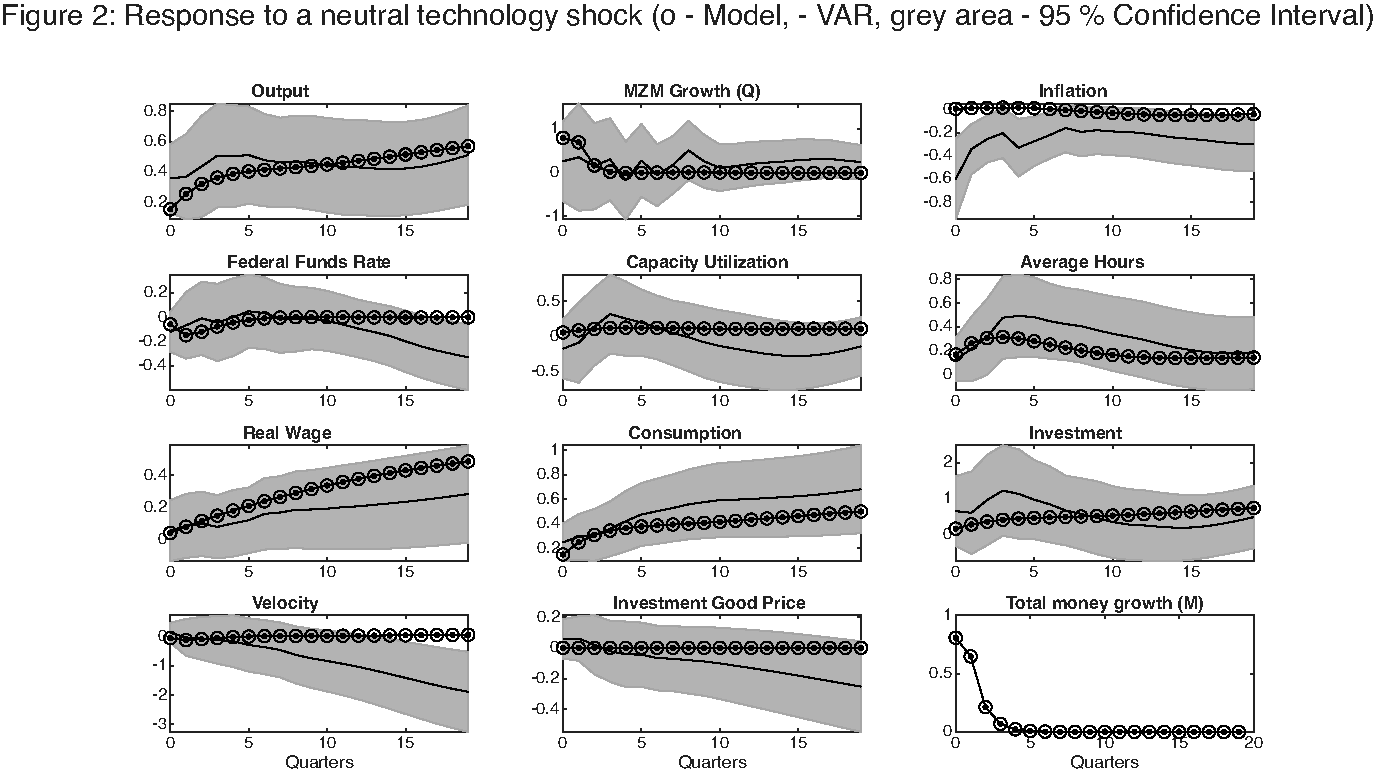
\includegraphics[width=1\linewidth]{../../Output/LDC_ACEL2011_Impulse_Response_Matching/NT_basic_DSGE/NT_DSGE4_lag_4.pdf}}
        {\fbox{Image Path Broken or File Missing}}
    \caption{Neutral Technology Shock DSGE matched with VAR lag 4 compared to VAR lag 4}
    \label{fig:basic_nt_lag4}
\end{figure}

\begin{figure}[htpb]
    \centering
    \IfFileExists{../../Output/LDC_ACEL2011_Impulse_Response_Matching/NT_basic_DSGE/NT_DSGE4_lag_6.pdf}
        {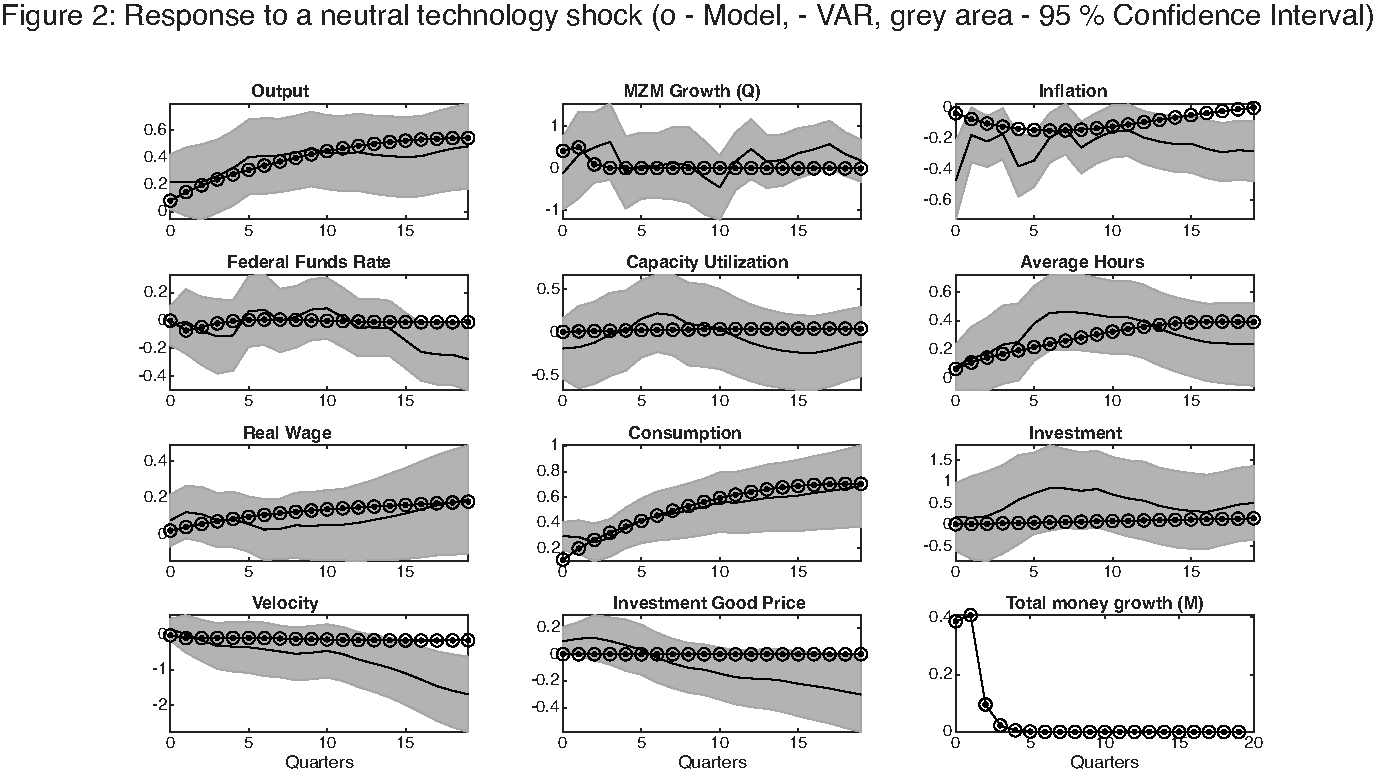
\includegraphics[width=1\linewidth]{../../Output/LDC_ACEL2011_Impulse_Response_Matching/NT_basic_DSGE/NT_DSGE4_lag_6.pdf}}
        {\fbox{Image Path Broken or File Missing}}
    \caption{Neutral Technology Shock DSGE matched with VAR lag 4 compared to VAR lag 6}
    \label{fig:basic_nt_lag6}
\end{figure}

\begin{figure}[htpb]
    \centering
    \IfFileExists{../../Output/LDC_ACEL2011_Impulse_Response_Matching/NT_basic_DSGE/NT_DSGE4_lag_8.pdf}
        {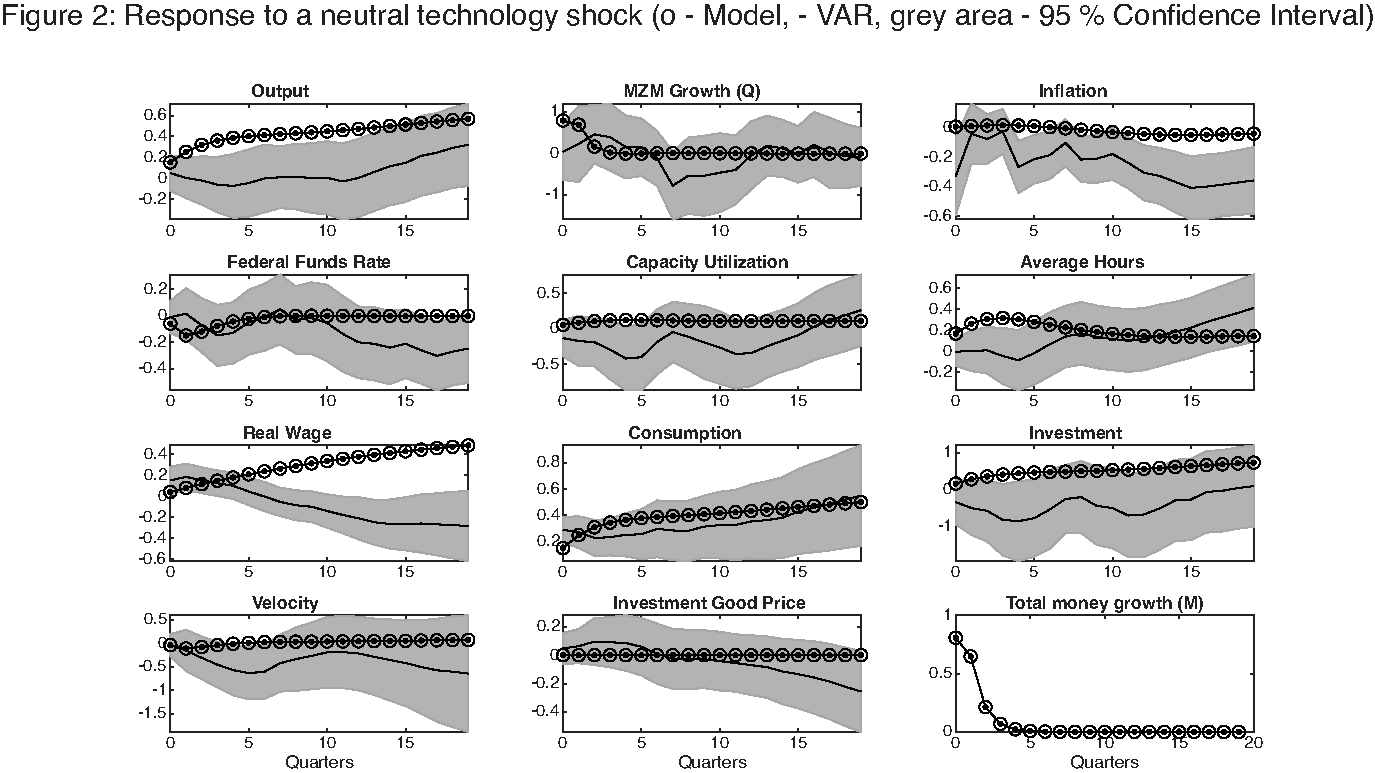
\includegraphics[width=1\linewidth]{../../Output/LDC_ACEL2011_Impulse_Response_Matching/NT_basic_DSGE/NT_DSGE4_lag_8.pdf}}
        {\fbox{Image Path Broken or File Missing}}
    \caption{Neutral Technology Shock DSGE matched with VAR lag 4 compared to VAR lag 8}
    \label{fig:basic_nt_lag8}
\end{figure}

\begin{figure}[htpb]
    \centering
    \IfFileExists{../../Output/LDC_ACEL2011_Impulse_Response_Matching/NT_basic_DSGE/NT_DSGE4_lag_10.pdf}
        {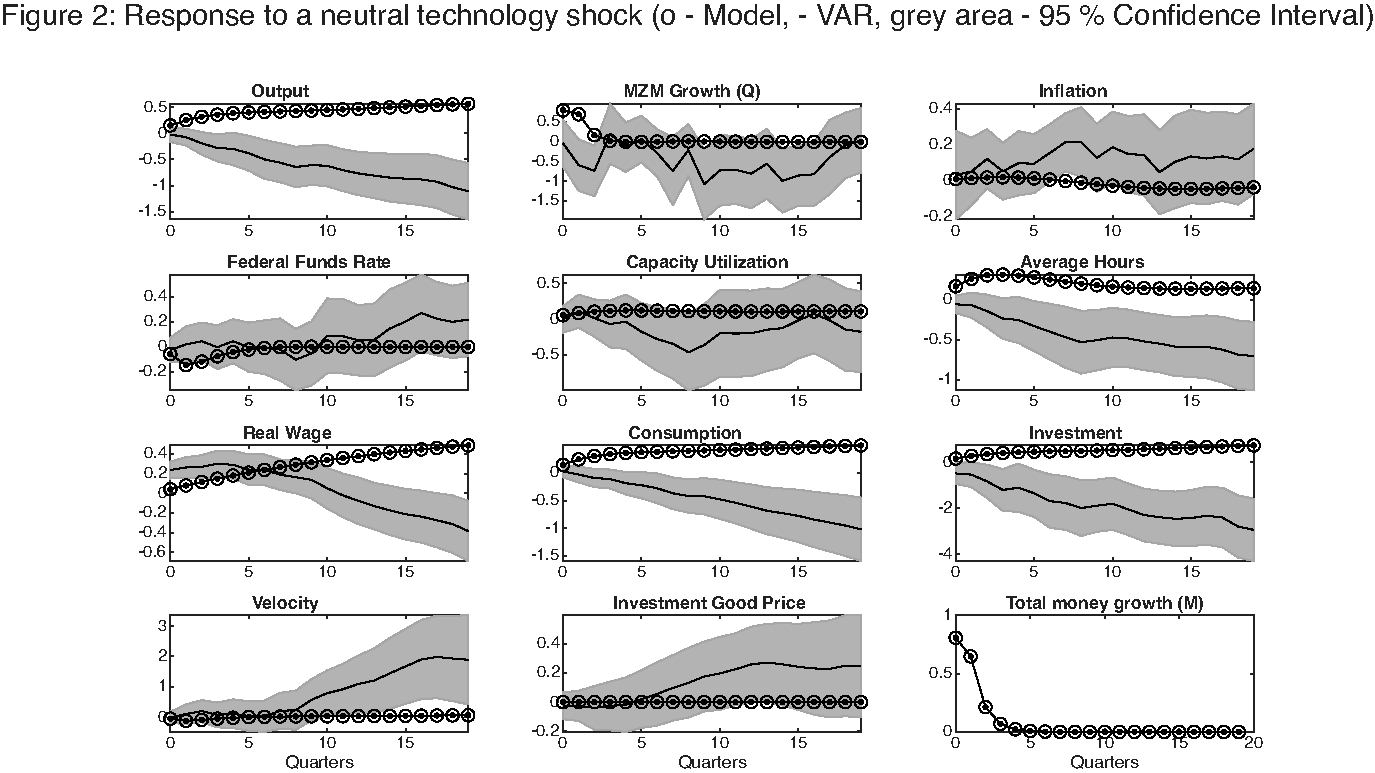
\includegraphics[width=1\linewidth]{../../Output/LDC_ACEL2011_Impulse_Response_Matching/NT_basic_DSGE/NT_DSGE4_lag_10.pdf}}
        {\fbox{Image Path Broken or File Missing}}
    \caption{Neutral Technology Shock DSGE matched with VAR lag 4 compared to VAR lag 10}
    \label{fig:basic_nt_lag10}
\end{figure}

\begin{figure}[htpb]
    \centering
    \IfFileExists{../../Output/LDC_ACEL2011_Impulse_Response_Matching/NT_basic_DSGE/NT_DSGE4_lag_12.pdf}
        {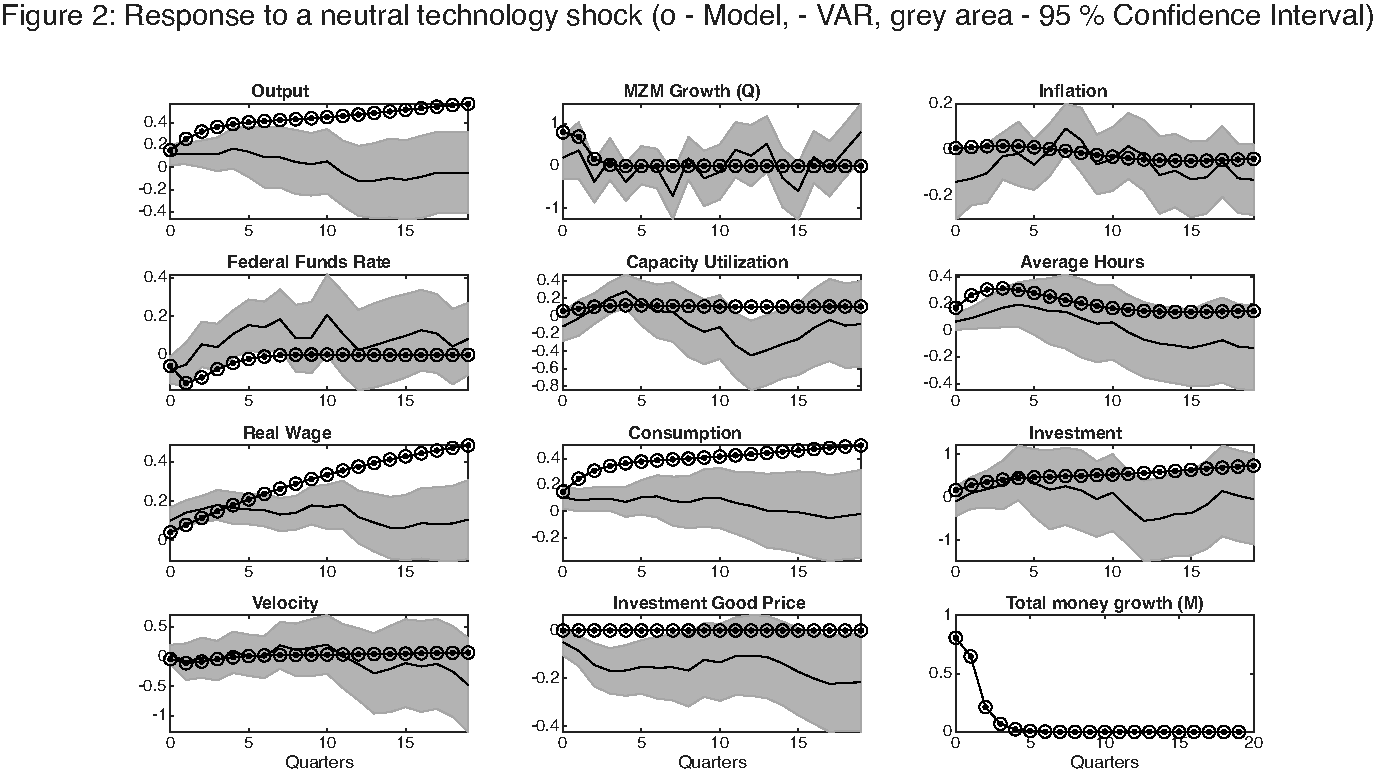
\includegraphics[width=1\linewidth]{../../Output/LDC_ACEL2011_Impulse_Response_Matching/NT_basic_DSGE/NT_DSGE4_lag_12.pdf}}
        {\fbox{Image Path Broken or File Missing}}
    \caption{Neutral Technology Shock DSGE matched with VAR lag 4 compared to VAR lag 12}
    \label{fig:basic_nt_lag12}
\end{figure}

\FloatBarrier

\clearpage

\subsection{ACEL 2005 DSGE Matched and compared with VAR estimated across different lag structures: Monetary Policy Shock}

\begin{figure}[htpb]
    \centering
    \IfFileExists{../../Output/LDC_ACEL2011_Impulse_Response_Matching/MP_matched_new_DSGE/MP_newDSGE_lag_4.pdf}
        {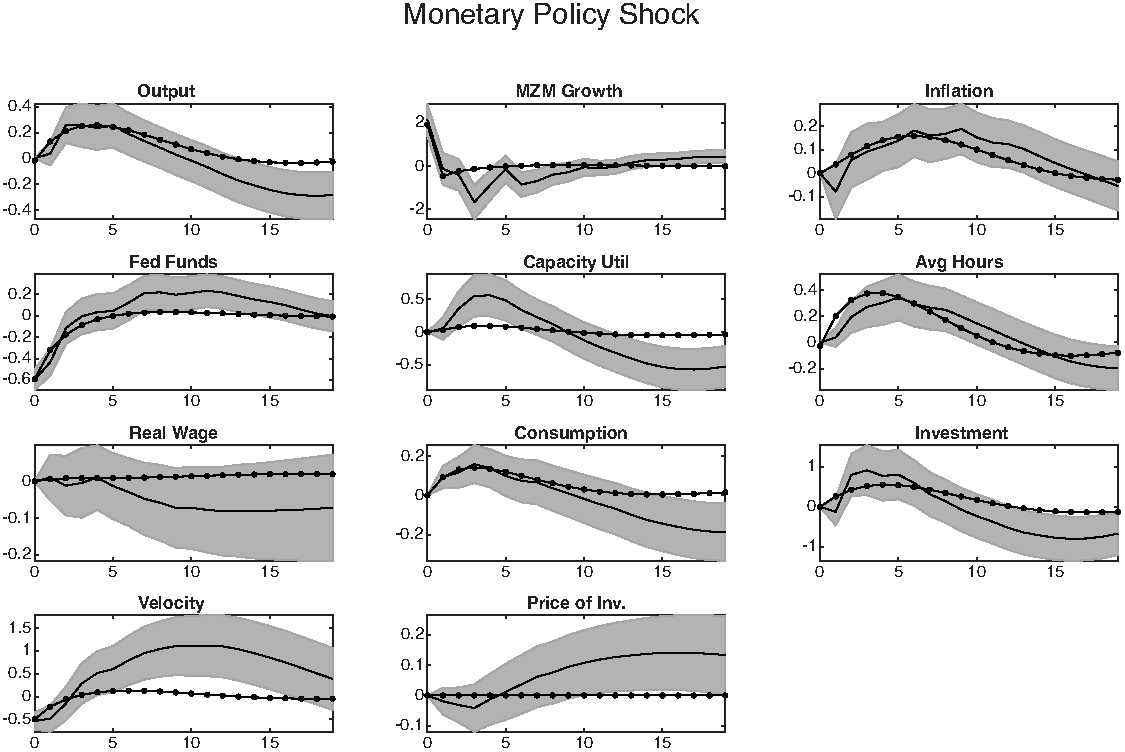
\includegraphics[width=1\linewidth]{../../Output/LDC_ACEL2011_Impulse_Response_Matching/MP_matched_new_DSGE/MP_newDSGE_lag_4.pdf}}
        {\fbox{Image Path Broken or File Missing}}
    \caption{Monetary Policy Shock DSGE matched with VAR lag 4 compared to VAR lag 4}
    \label{fig:new_mp_lag4}
\end{figure}

\begin{figure}[htpb]
    \centering
    \IfFileExists{../../Output/LDC_ACEL2011_Impulse_Response_Matching/MP_matched_new_DSGE/MP_newDSGE_lag_6.pdf}
        {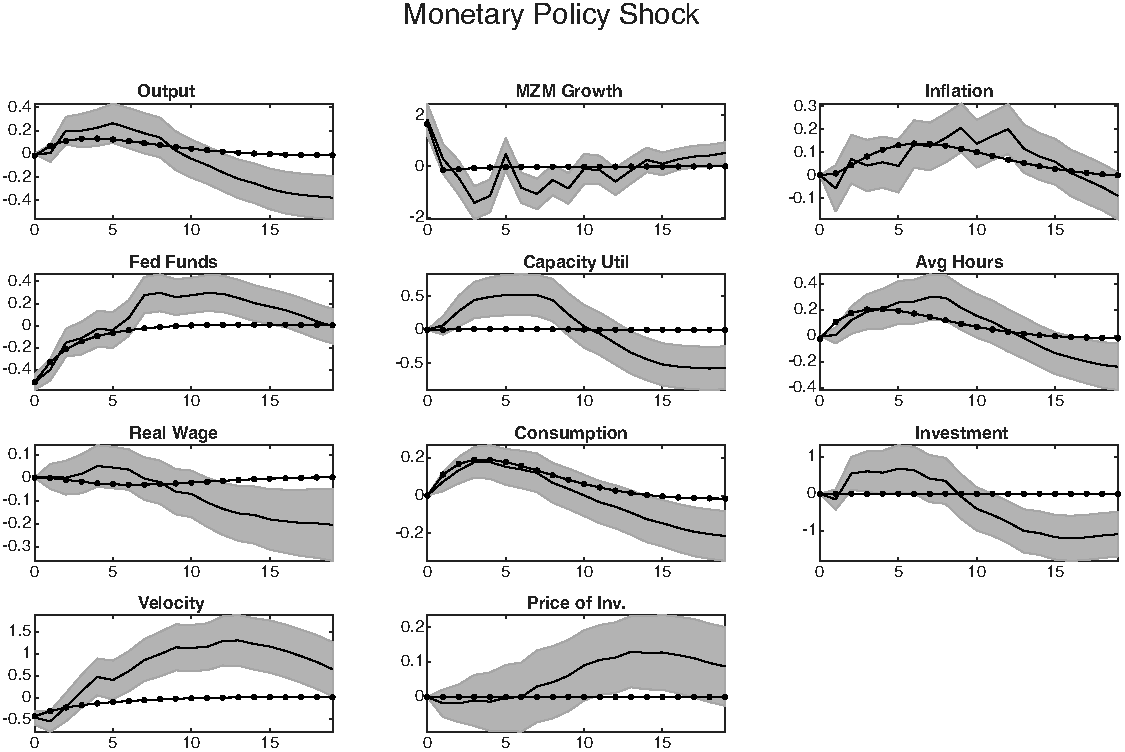
\includegraphics[width=1\linewidth]{../../Output/LDC_ACEL2011_Impulse_Response_Matching/MP_matched_new_DSGE/MP_newDSGE_lag_6.pdf}}
        {\fbox{Image Path Broken or File Missing}}
    \caption{Monetary Policy Shock DSGE matched with VAR lag 6 compared to VAR lag 6}
    \label{fig:new_mp_lag6}
\end{figure}

\begin{figure}[htpb]
    \centering
    \IfFileExists{../../Output/LDC_ACEL2011_Impulse_Response_Matching/MP_matched_new_DSGE/MP_newDSGE_lag_8.pdf}
        {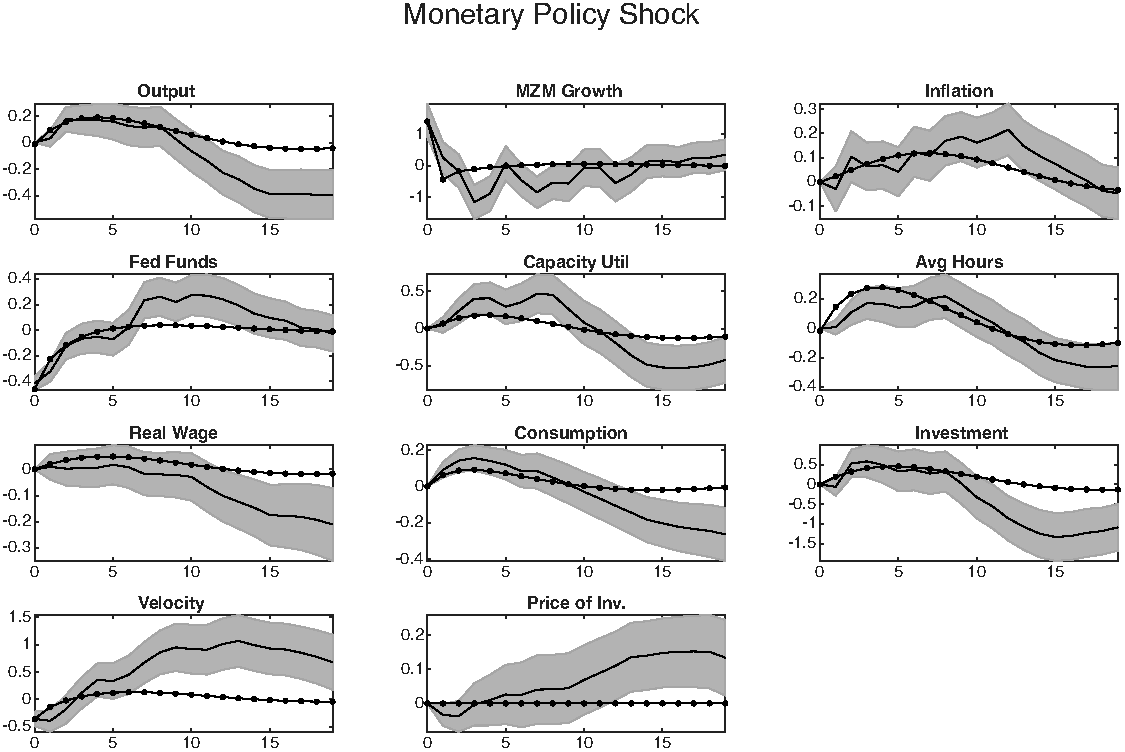
\includegraphics[width=1\linewidth]{../../Output/LDC_ACEL2011_Impulse_Response_Matching/MP_matched_new_DSGE/MP_newDSGE_lag_8.pdf}}
        {\fbox{Image Path Broken or File Missing}}
    \caption{Monetary Policy Shock DSGE matched with VAR lag 8 compared to VAR lag 8}
    \label{fig:new_mp_lag8}
\end{figure}

\begin{figure}[htpb]
    \centering
    \IfFileExists{../../Output/LDC_ACEL2011_Impulse_Response_Matching/MP_matched_new_DSGE/MP_newDSGE_lag_10.pdf}
        {\includegraphics[width=1\linewidth]{../../Output/LDC_ACEL2011_Impulse_Response_Matching/MP_matched_new_DSGE/MP_newDSGE_lag_10.pdf}}
        {\fbox{Image Path Broken or File Missing}}
    \caption{Monetary Policy Shock DSGE matched with VAR lag 10 compared to VAR lag 10}
    \label{fig:new_mp_lag10}
\end{figure}

\begin{figure}[htpb]
    \centering
    \IfFileExists{../../Output/LDC_ACEL2011_Impulse_Response_Matching/MP_matched_new_DSGE/MP_newDSGE_lag_12.pdf}
        {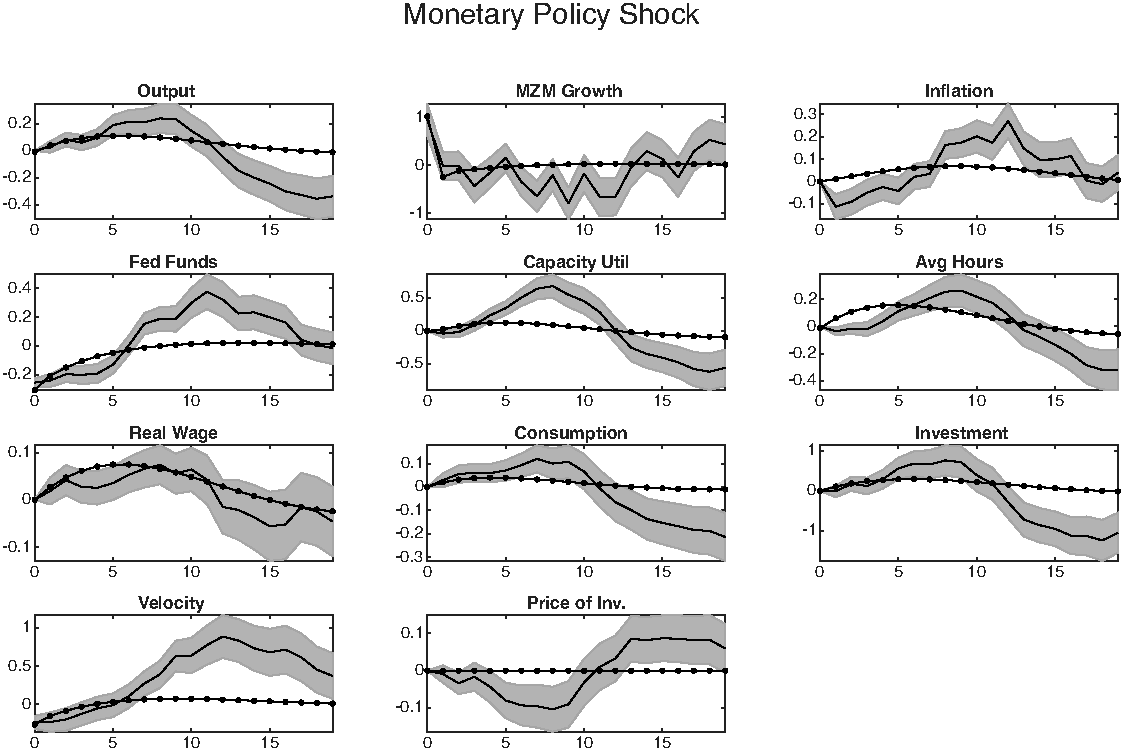
\includegraphics[width=1\linewidth]{../../Output/LDC_ACEL2011_Impulse_Response_Matching/MP_matched_new_DSGE/MP_newDSGE_lag_12.pdf}}
        {\fbox{Image Path Broken or File Missing}}
    \caption{Monetary Policy Shock DSGE matched with VAR lag 12 compared to VAR lag 12}
    \label{fig:new_mp_lag12}
\end{figure}

\FloatBarrier

\clearpage
\subsection{ACEL 2005 DSGE Matched and compared with VAR estimated across different lag structures: Embodied Technology Shock}

\begin{figure}[htpb]
    \centering
    \IfFileExists{../../Output/LDC_ACEL2011_Impulse_Response_Matching/ET_matched_new_DSGE/ET_newDSGE_lag_4.pdf}
        {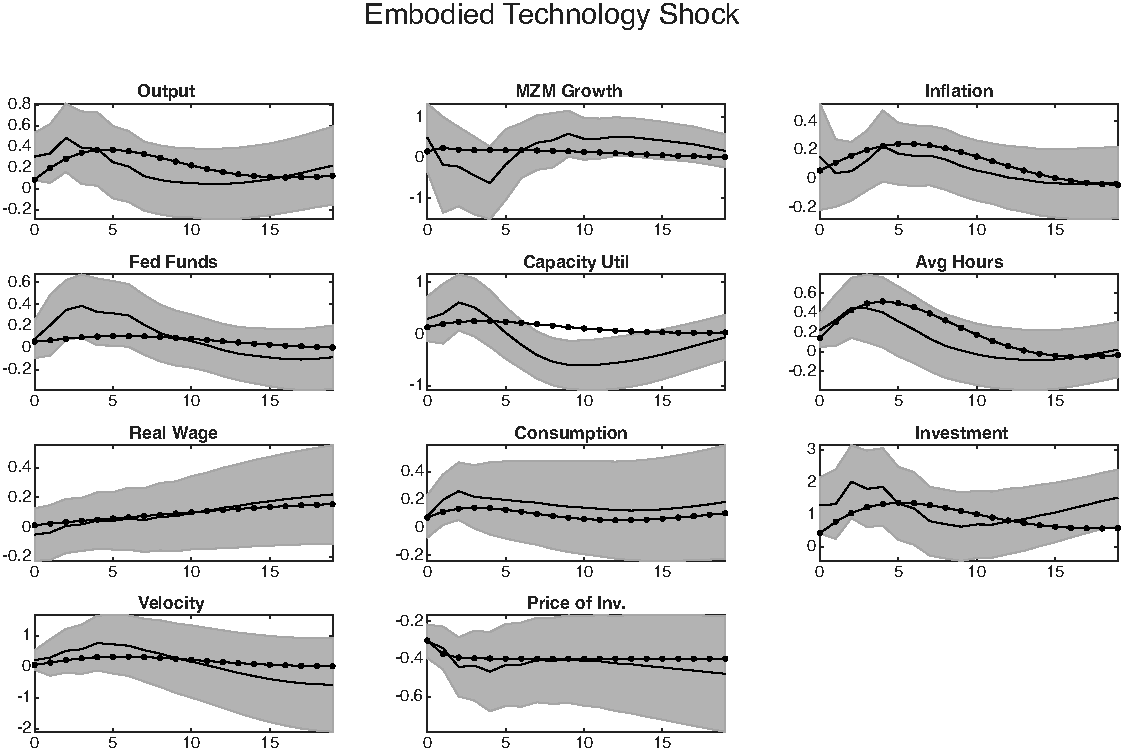
\includegraphics[width=1\linewidth]{../../Output/LDC_ACEL2011_Impulse_Response_Matching/ET_matched_new_DSGE/ET_newDSGE_lag_4.pdf}}
        {\fbox{Image Path Broken or File Missing}}
    \caption{Embodied Technology Shock DSGE matched with VAR lag 4 compared to VAR lag 4}
    \label{fig:new_et_lag4}
\end{figure}

\begin{figure}[htpb]
    \centering
    \IfFileExists{../../Output/LDC_ACEL2011_Impulse_Response_Matching/ET_matched_new_DSGE/ET_newDSGE_lag_6.pdf}
        {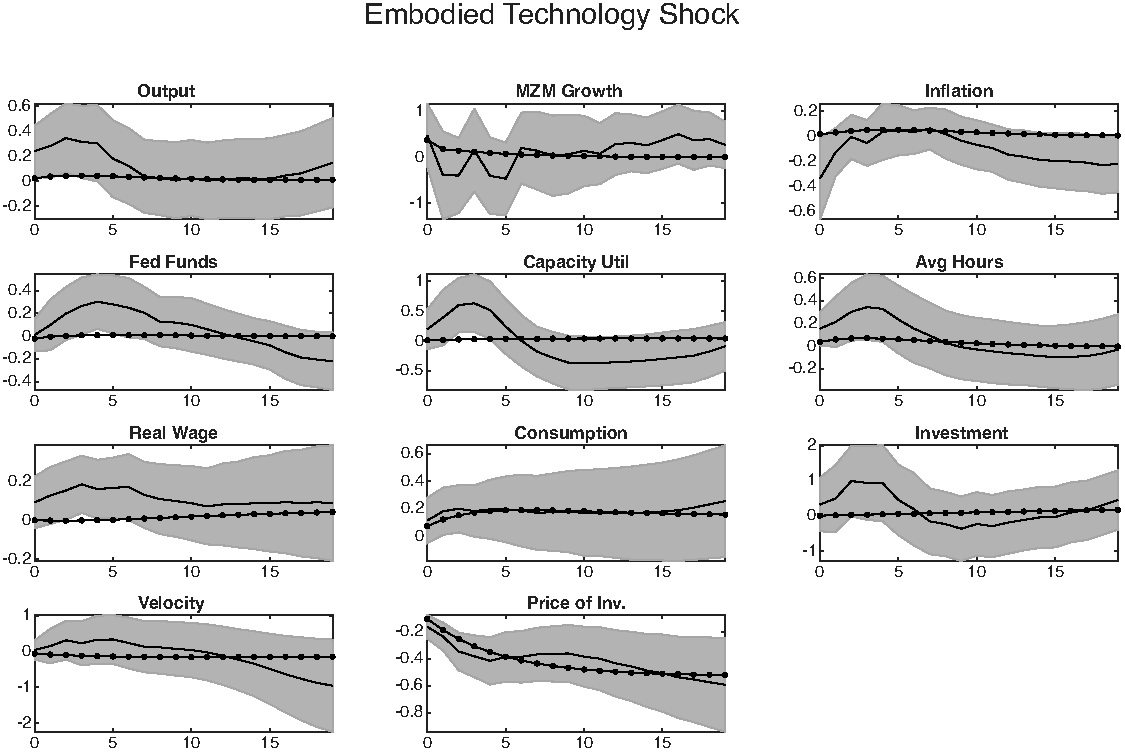
\includegraphics[width=1\linewidth]{../../Output/LDC_ACEL2011_Impulse_Response_Matching/ET_matched_new_DSGE/ET_newDSGE_lag_6.pdf}}
        {\fbox{Image Path Broken or File Missing}}
    \caption{Embodied Technology Shock DSGE matched with VAR lag 6 compared to VAR lag 6}
    \label{fig:new_et_lag6}
\end{figure}

\begin{figure}[htpb]
    \centering
    \IfFileExists{../../Output/LDC_ACEL2011_Impulse_Response_Matching/ET_matched_new_DSGE/ET_newDSGE_lag_8.pdf}
        {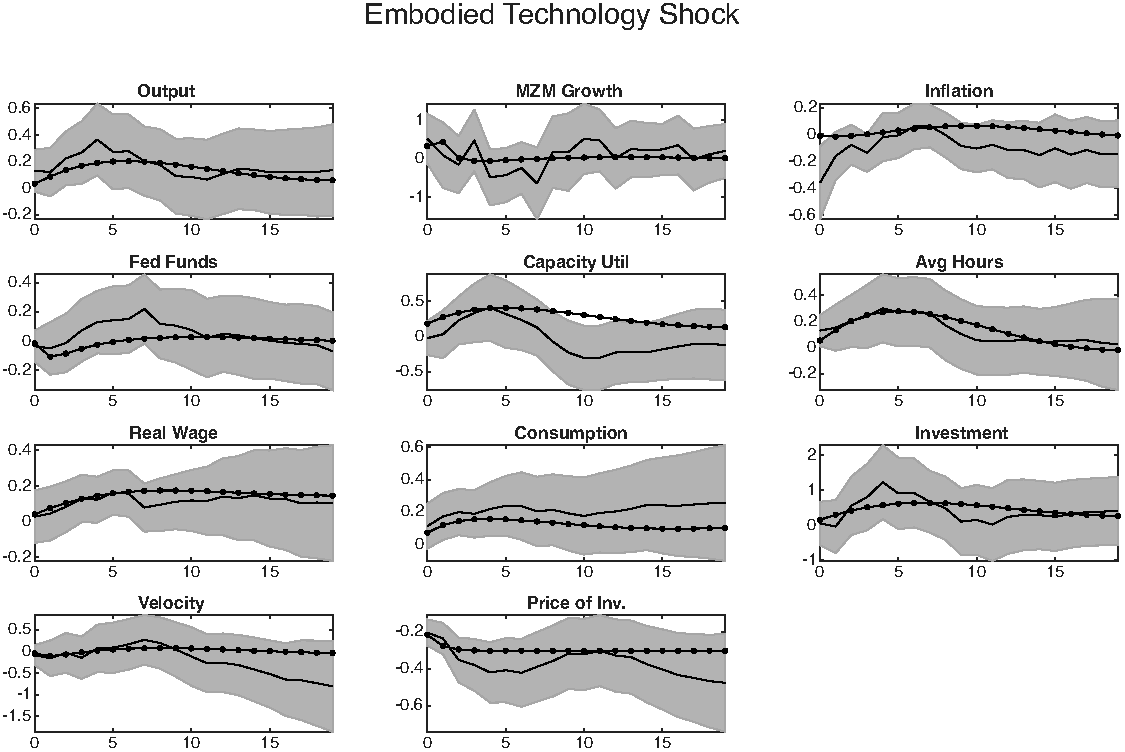
\includegraphics[width=1\linewidth]{../../Output/LDC_ACEL2011_Impulse_Response_Matching/ET_matched_new_DSGE/ET_newDSGE_lag_8.pdf}}
        {\fbox{Image Path Broken or File Missing}}
    \caption{Embodied Technology Shock DSGE matched with VAR lag 8 compared to VAR lag 8}
    \label{fig:new_et_lag8}
\end{figure}

\begin{figure}[htpb]
    \centering
    \IfFileExists{../../Output/LDC_ACEL2011_Impulse_Response_Matching/ET_matched_new_DSGE/ET_newDSGE_lag_10.pdf}
        {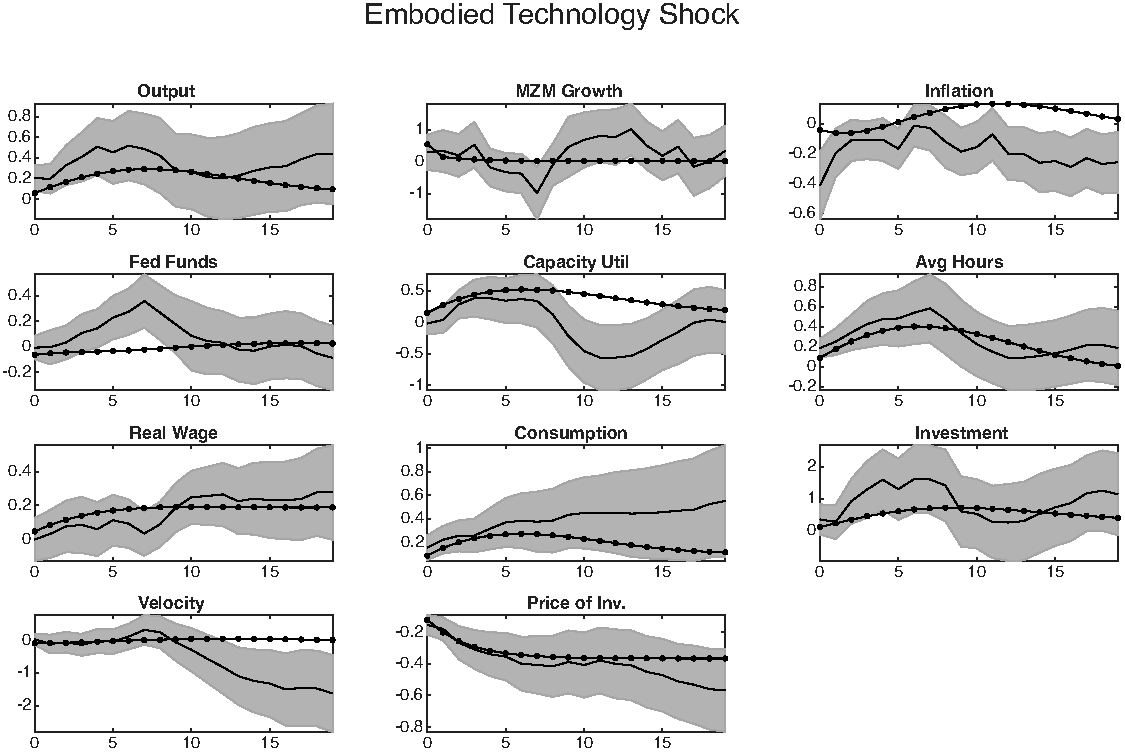
\includegraphics[width=1\linewidth]{../../Output/LDC_ACEL2011_Impulse_Response_Matching/ET_matched_new_DSGE/ET_newDSGE_lag_10.pdf}}
        {\fbox{Image Path Broken or File Missing}}
    \caption{Embodied Technology Shock DSGE matched with VAR lag 10 compared to VAR lag 10}
    \label{fig:new_et_lag10}
\end{figure}

\begin{figure}[htpb]
    \centering
    \IfFileExists{../../Output/LDC_ACEL2011_Impulse_Response_Matching/ET_matched_new_DSGE/ET_newDSGE_lag_12.pdf}
        {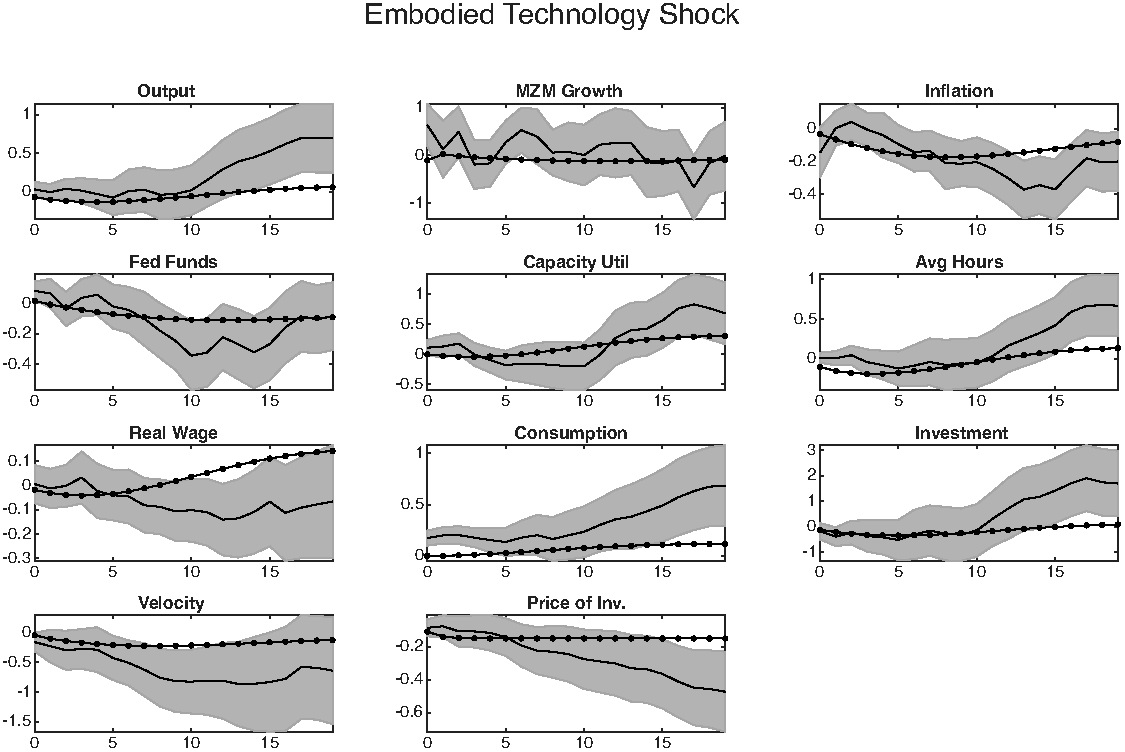
\includegraphics[width=1\linewidth]{../../Output/LDC_ACEL2011_Impulse_Response_Matching/ET_matched_new_DSGE/ET_newDSGE_lag_12.pdf}}
        {\fbox{Image Path Broken or File Missing}}
    \caption{Embodied Technology Shock DSGE matched with VAR lag 12 compared to VAR lag 12}
    \label{fig:new_et_lag12}
\end{figure}

\FloatBarrier

\clearpage
\subsection{ACEL 2005 DSGE Matched and compared with VAR estimated across different lag structures: Neutral Technology Shock}

\begin{figure}[htpb]
    \centering
    \IfFileExists{../../Output/LDC_ACEL2011_Impulse_Response_Matching/NT_matched_new_DSGE/NT_newDSGE_lag_4.pdf}
        {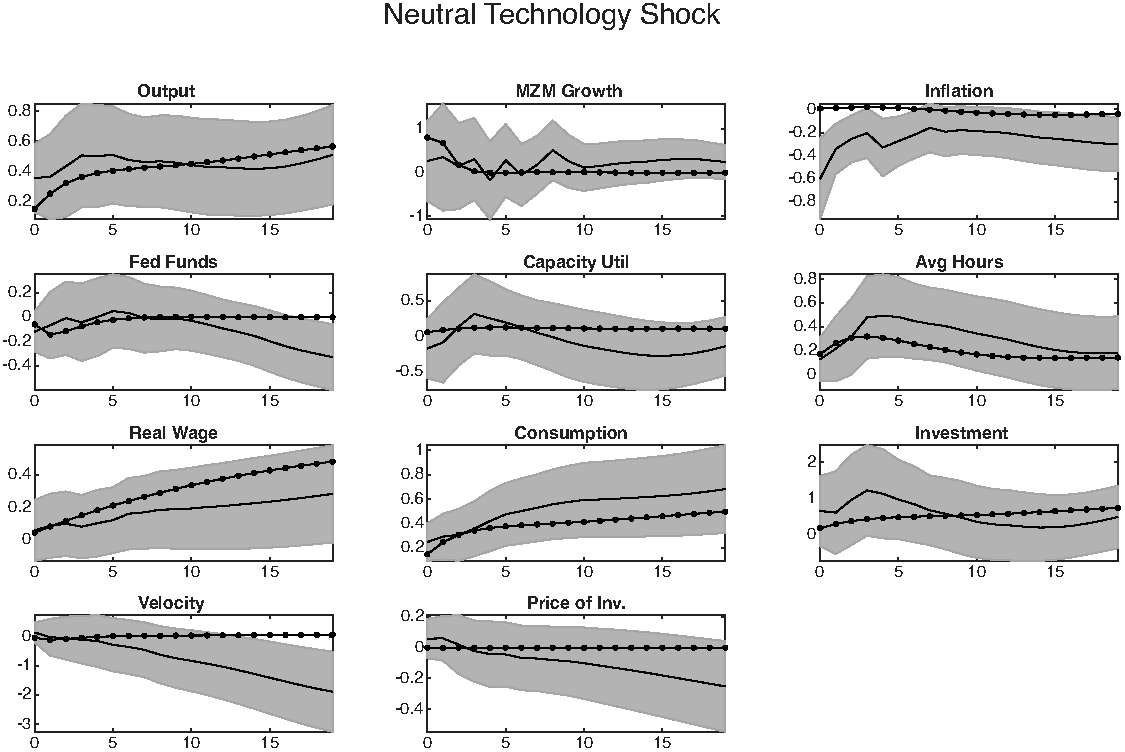
\includegraphics[width=1\linewidth]{../../Output/LDC_ACEL2011_Impulse_Response_Matching/NT_matched_new_DSGE/NT_newDSGE_lag_4.pdf}}
        {\fbox{Image Path Broken or File Missing}}
    \caption{Neutral Technology Shock DSGE matched with VAR lag 4 compared to VAR lag 4}
    \label{fig:new_nt_lag4}
\end{figure}

\begin{figure}[htpb]
    \centering
    \IfFileExists{../../Output/LDC_ACEL2011_Impulse_Response_Matching/NT_matched_new_DSGE/NT_newDSGE_lag_6.pdf}
        {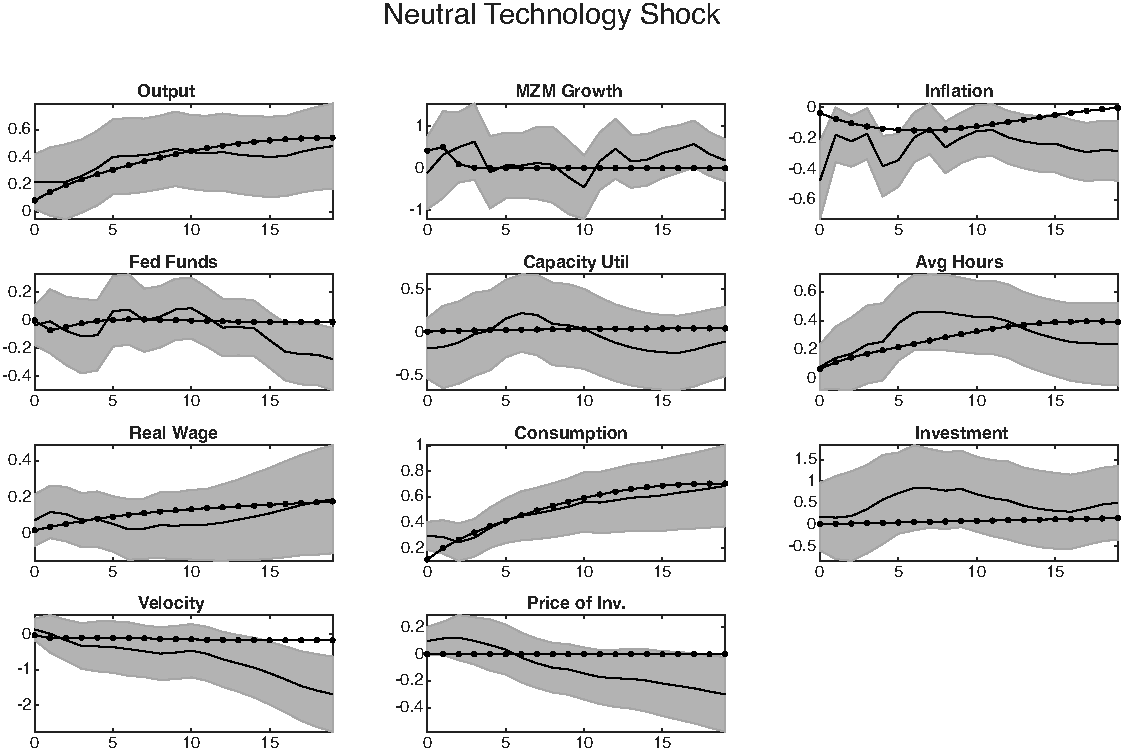
\includegraphics[width=1\linewidth]{../../Output/LDC_ACEL2011_Impulse_Response_Matching/NT_matched_new_DSGE/NT_newDSGE_lag_6.pdf}}
        {\fbox{Image Path Broken or File Missing}}
    \caption{Neutral Technology Shock DSGE matched with VAR lag 6 compared to VAR lag 6}
    \label{fig:new_nt_lag6}
\end{figure}

\begin{figure}[htpb]
    \centering
    \IfFileExists{../../Output/LDC_ACEL2011_Impulse_Response_Matching/NT_matched_new_DSGE/NT_newDSGE_lag_8.pdf}
        {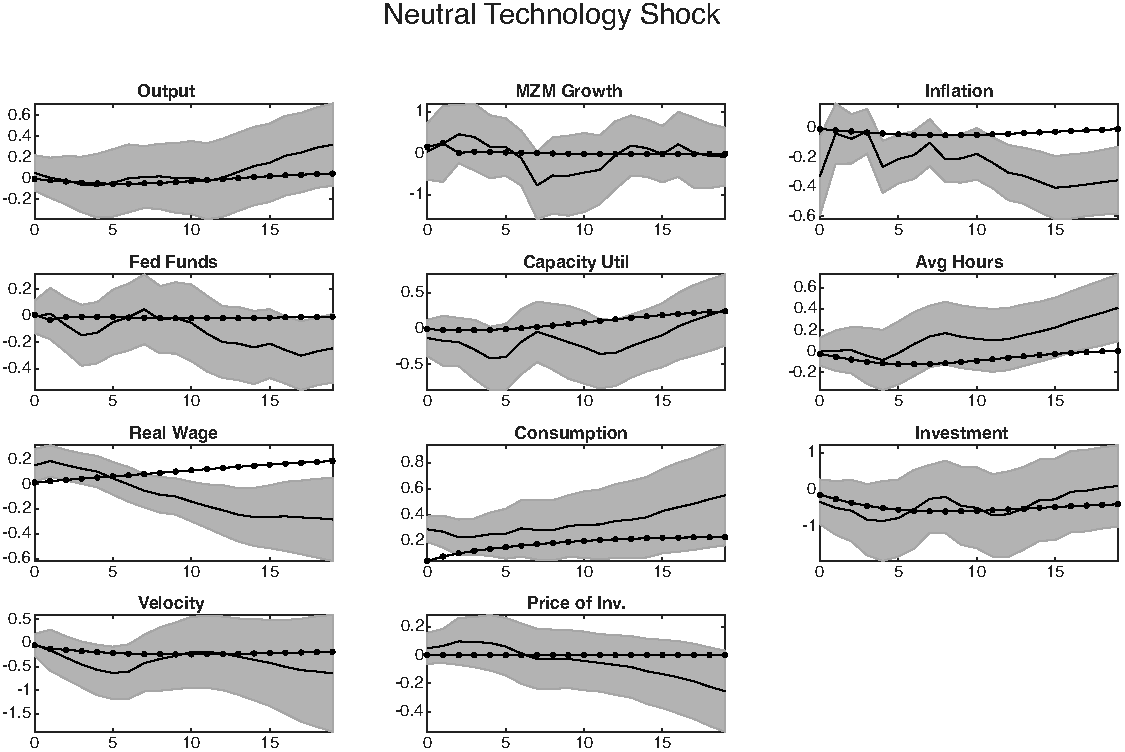
\includegraphics[width=1\linewidth]{../../Output/LDC_ACEL2011_Impulse_Response_Matching/NT_matched_new_DSGE/NT_newDSGE_lag_8.pdf}}
        {\fbox{Image Path Broken or File Missing}}
    \caption{Neutral Technology Shock DSGE matched with VAR lag 8 compared to VAR lag 8}
    \label{fig:new_nt_lag8}
\end{figure}

\begin{figure}[htpb]
    \centering
    \IfFileExists{../../Output/LDC_ACEL2011_Impulse_Response_Matching/NT_matched_new_DSGE/NT_newDSGE_lag_10.pdf}
        {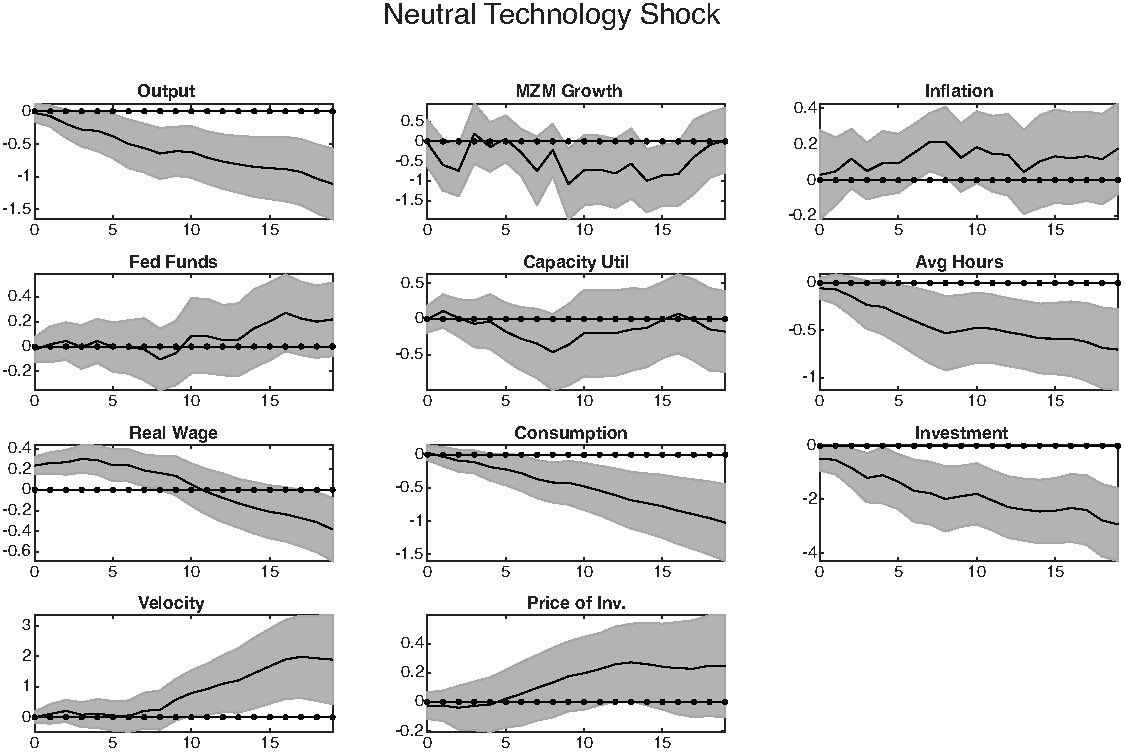
\includegraphics[width=1\linewidth]{../../Output/LDC_ACEL2011_Impulse_Response_Matching/NT_matched_new_DSGE/NT_newDSGE_lag_10.pdf}}
        {\fbox{Image Path Broken or File Missing}}
    \caption{Neutral Technology Shock DSGE matched with VAR lag 10 compared to VAR lag 10}
    \label{fig:new_nt_lag10}
\end{figure}

\begin{figure}[htpb]
    \centering
    \IfFileExists{../../Output/LDC_ACEL2011_Impulse_Response_Matching/NT_matched_new_DSGE/NT_newDSGE_lag_12.pdf}
        {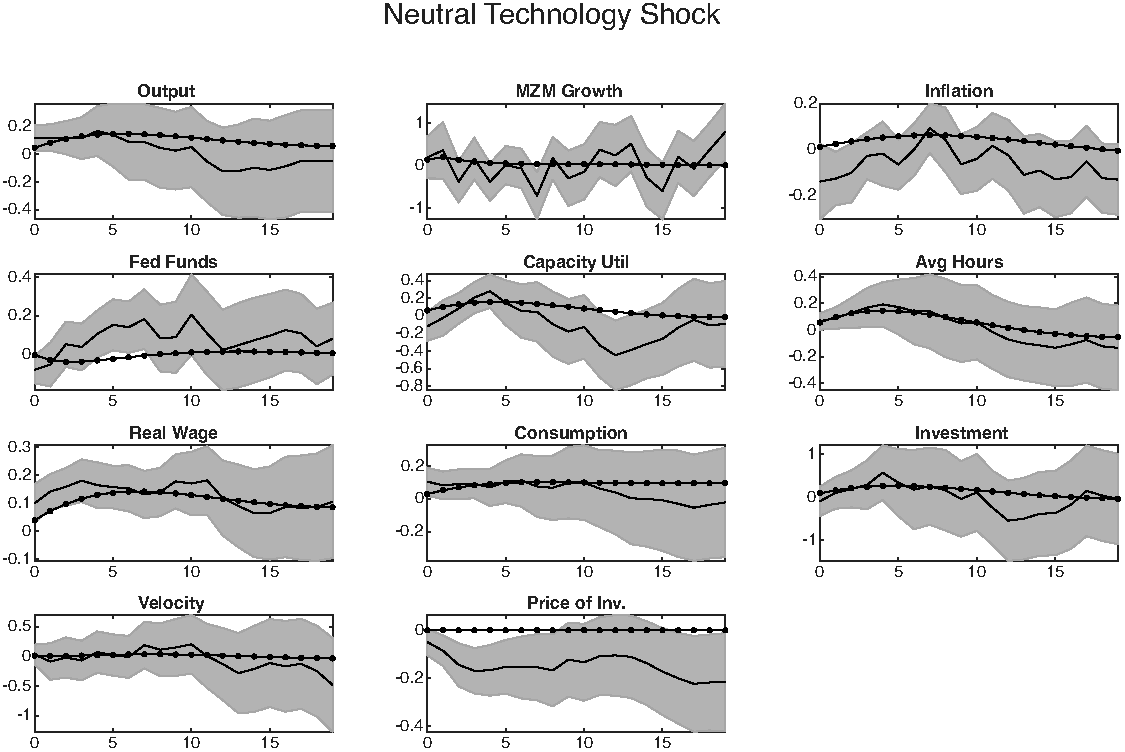
\includegraphics[width=1\linewidth]{../../Output/LDC_ACEL2011_Impulse_Response_Matching/NT_matched_new_DSGE/NT_newDSGE_lag_12.pdf}}
        {\fbox{Image Path Broken or File Missing}}
    \caption{Neutral Technology Shock DSGE matched with VAR lag 12 compared to VAR lag 12}
    \label{fig:new_nt_lag12}
\end{figure}

\FloatBarrier

\subsection{VAR Residual Analysis}

\begin{figure}[htpb]
    \centering
    \IfFileExists{../../Output/VAR_Residuals_RMSE_Estimates/InSample_Residuals_VAR4_Vs_VAR12_All_Variables.pdf}
        {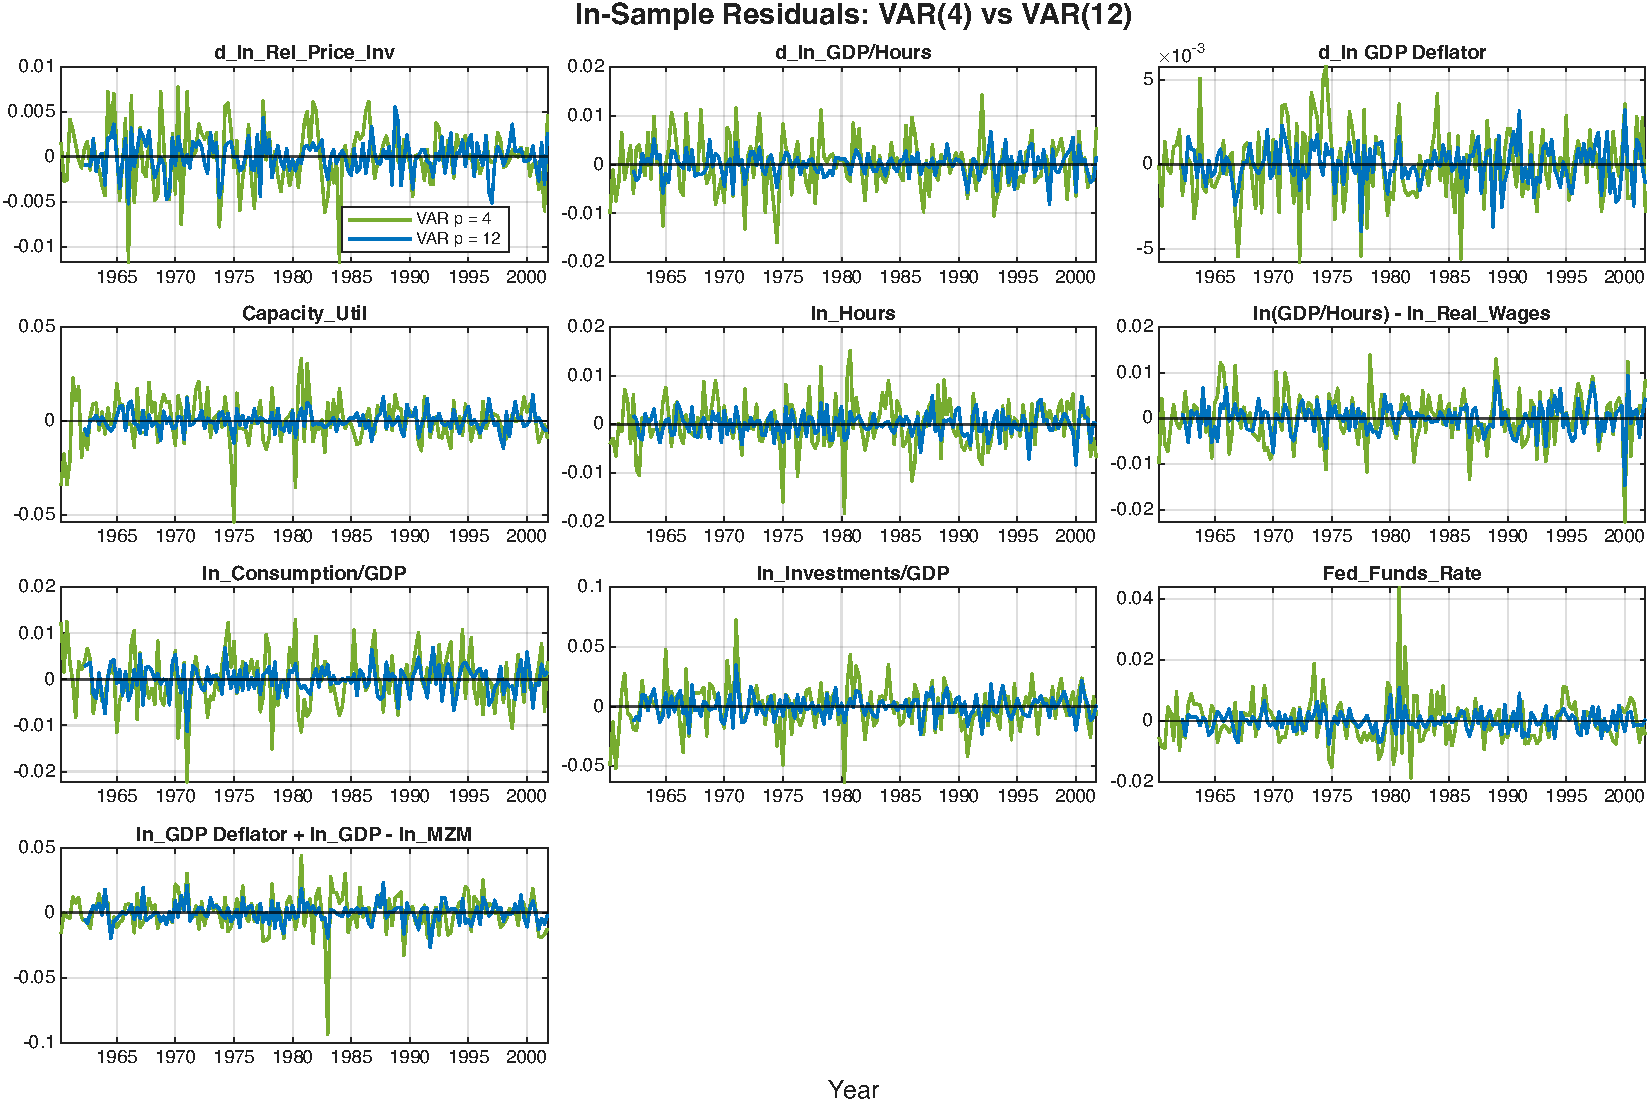
\includegraphics[width=1\linewidth]{../../Output/VAR_Residuals_RMSE_Estimates/InSample_Residuals_VAR4_Vs_VAR12_All_Variables.pdf}}
        {\fbox{Image Path Broken or File Missing}}
    \caption{VAR Residuals Comparison: VAR(4) vs VAR(12)}
    \label{fig:var_residuals}
\end{figure}

\begin{figure}[htpb]
    \centering
    \IfFileExists{../../Output/VAR_Residuals_RMSE_Estimates/InSample_RMSE__Across_Lags_All_Variables.pdf}
        {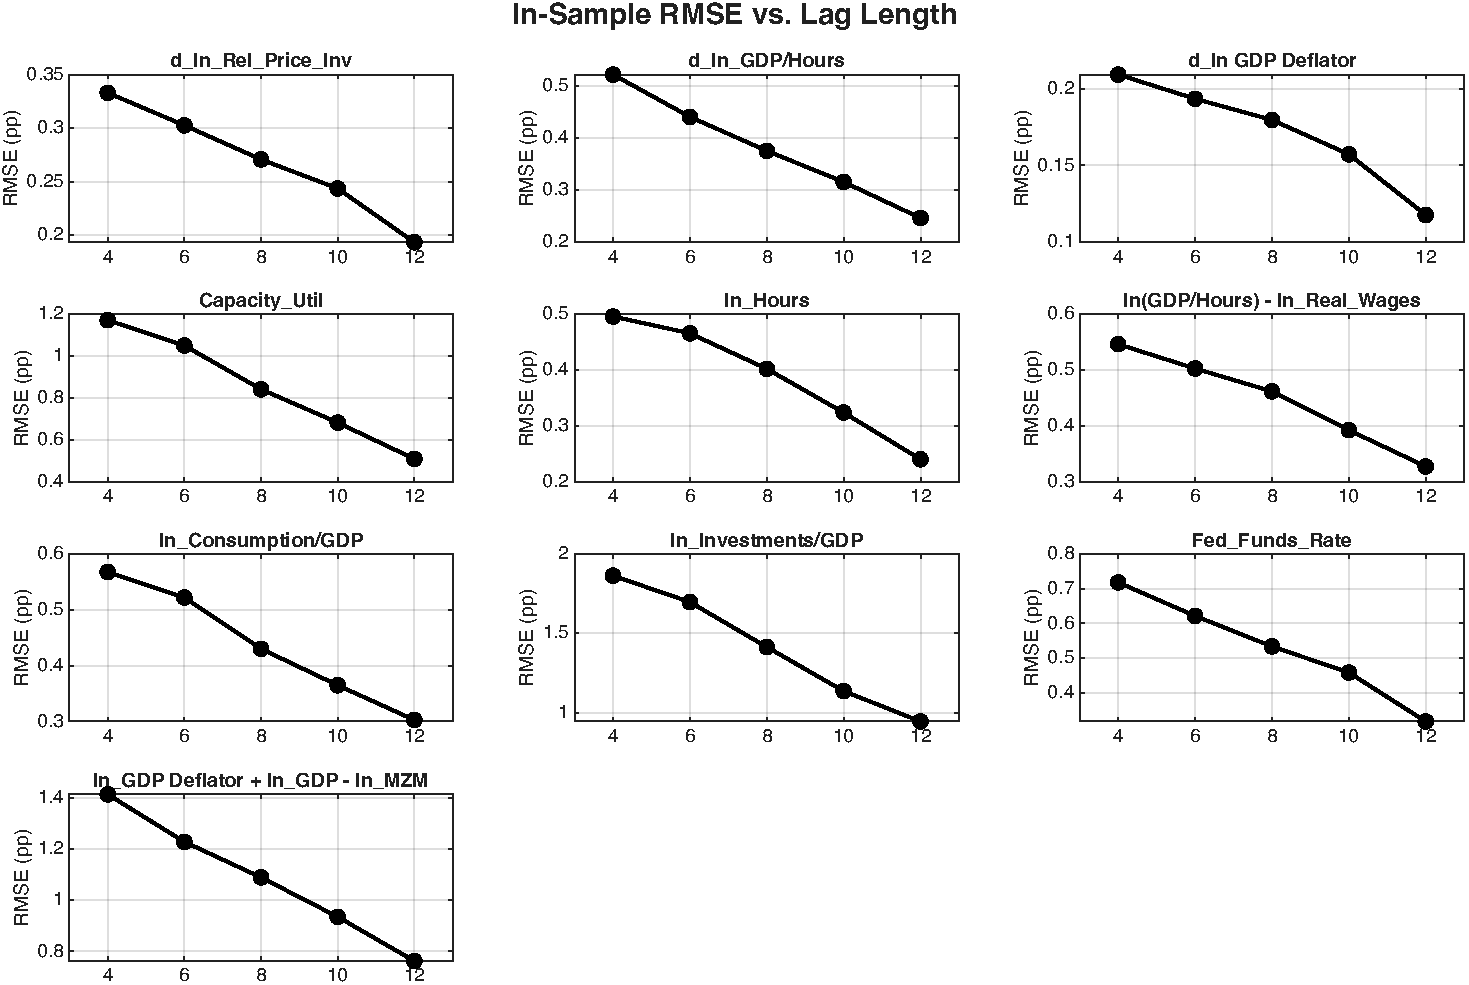
\includegraphics[width=1\linewidth]{../../Output/VAR_Residuals_RMSE_Estimates/InSample_RMSE__Across_Lags_All_Variables.pdf}}
        {\fbox{Image Path Broken or File Missing}}
    \caption{VAR RMSE Comparison across different lag structures}
    \label{fig:var_residuals}
\end{figure}

\begin{figure}[htpb]
    \centering
    \IfFileExists{../../Output/Residual_Analysis_Output/Ljung_Box_P_Values_Across_VAR_lags.pdf}
        {\includegraphics[width=1\linewidth]{../../Output/Residual_Analysis_Output/Ljung_Box_P_Values_Across_VAR_lags.pdf}}
        {\fbox{Image Path Broken or File Missing}}
    \caption{Ljung-Box P-Values Across VAR Lags}
    \label{fig:ljung_box}
\end{figure}

\begin{figure}[htpb]
    \centering
    \IfFileExists{../../Output/Residual_Analysis_Output/Standard_Deviation_Ratios.pdf}
        {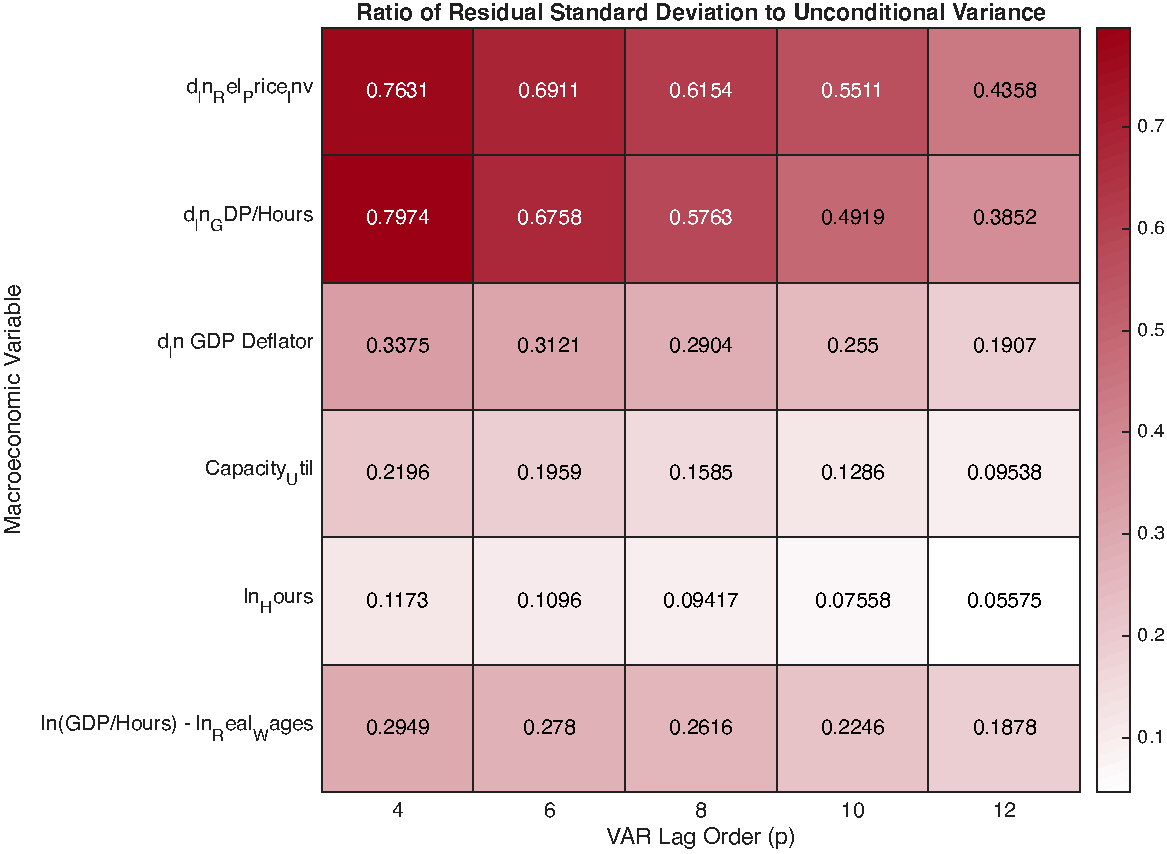
\includegraphics[width=1\linewidth]{../../Output/Residual_Analysis_Output/Standard_Deviation_Ratios.pdf}}
        {\fbox{Image Path Broken or File Missing}}
    \caption{Standard Deviation Ratios}
    \label{fig:std_dev_ratios}
\end{figure}

\FloatBarrier

\subsection{ACEL 2005 VAR Across different lag structures Progressively Comparison: Monetary Policy Shock}

\begin{figure}[htpb]
    \centering
    \IfFileExists{../../Output/VAR_IRFs_Long_Lag_Progressively_Plots/Monetary_policy_Shock/Step_1_UpToLag_4.pdf}
    {\includegraphics[width=1\linewidth]{../../Output/VAR_IRFs_Long_Lag_Progressively_Plots/Monetary_policy_Shock/Step_1_UpToLag_4.pdf}}{\fbox{Image Path Broken or File Missing}}
    \caption{Monetary Policy Shock lag 4}
    \label{fig:VAR_mp_baseline_lag4}
\end{figure}

\begin{figure}[htpb]
    \centering
    \IfFileExists{../../Output/VAR_IRFs_Long_Lag_Progressively_Plots/Monetary_policy_Shock/Step_2_UpToLag_6.pdf}
    {\includegraphics[width=1\linewidth]{../../Output/VAR_IRFs_Long_Lag_Progressively_Plots/Monetary_policy_Shock/Step_2_UpToLag_6.pdf}}{\fbox{Image Path Broken or File Missing}}
    \caption{Monetary Policy Shock lag 6}
    \label{fig:VAR_mp_baseline_lag6}
\end{figure}

\begin{figure}[htpb]
    \centering
    \IfFileExists{../../Output/VAR_IRFs_Long_Lag_Progressively_Plots/Monetary_policy_Shock/Step_3_UpToLag_8.pdf}
    {\includegraphics[width=1\linewidth]{../../Output/VAR_IRFs_Long_Lag_Progressively_Plots/Monetary_policy_Shock/Step_3_UpToLag_8.pdf}}{\fbox{Image Path Broken or File Missing}}
    \caption{Monetary Policy Shock lag 8}
    \label{fig:VAR_mp_baseline_lag8}
\end{figure}

\begin{figure}[htpb]
    \centering
    \IfFileExists{../../Output/VAR_IRFs_Long_Lag_Progressively_Plots/Monetary_policy_Shock/Step_4_UpToLag_10.pdf}
    {\includegraphics[width=1\linewidth]{../../Output/VAR_IRFs_Long_Lag_Progressively_Plots/Monetary_policy_Shock/Step_4_UpToLag_10.pdf}}{\fbox{Image Path Broken or File Missing}}
    \caption{Monetary Policy Shock lag 10}
    \label{fig:VAR_mp_baseline_lag10}
\end{figure}

\begin{figure}[htpb]
    \centering
    \IfFileExists{../../Output/VAR_IRFs_Long_Lag_Progressively_Plots/Monetary_policy_Shock/Step_5_UpToLag_12.pdf}
    {\includegraphics[width=1\linewidth]{../../Output/VAR_IRFs_Long_Lag_Progressively_Plots/Monetary_policy_Shock/Step_5_UpToLag_12.pdf}}{\fbox{Image Path Broken or File Missing}}
    \caption{Monetary Policy Shock lag 12}
    \label{fig:VAR_mp_baseline_lag12}
\end{figure}

\FloatBarrier
\subsection{ACEL 2005 VAR Across different lag structures Progressively Comparison: Embodied Technology Shock}

\begin{figure}[htpb]
    \centering
    \IfFileExists{../../Output/VAR_IRFs_Long_Lag_Progressively_Plots/Embodied_Technology_Shock/Step_1_UpToLag_4.pdf}
    {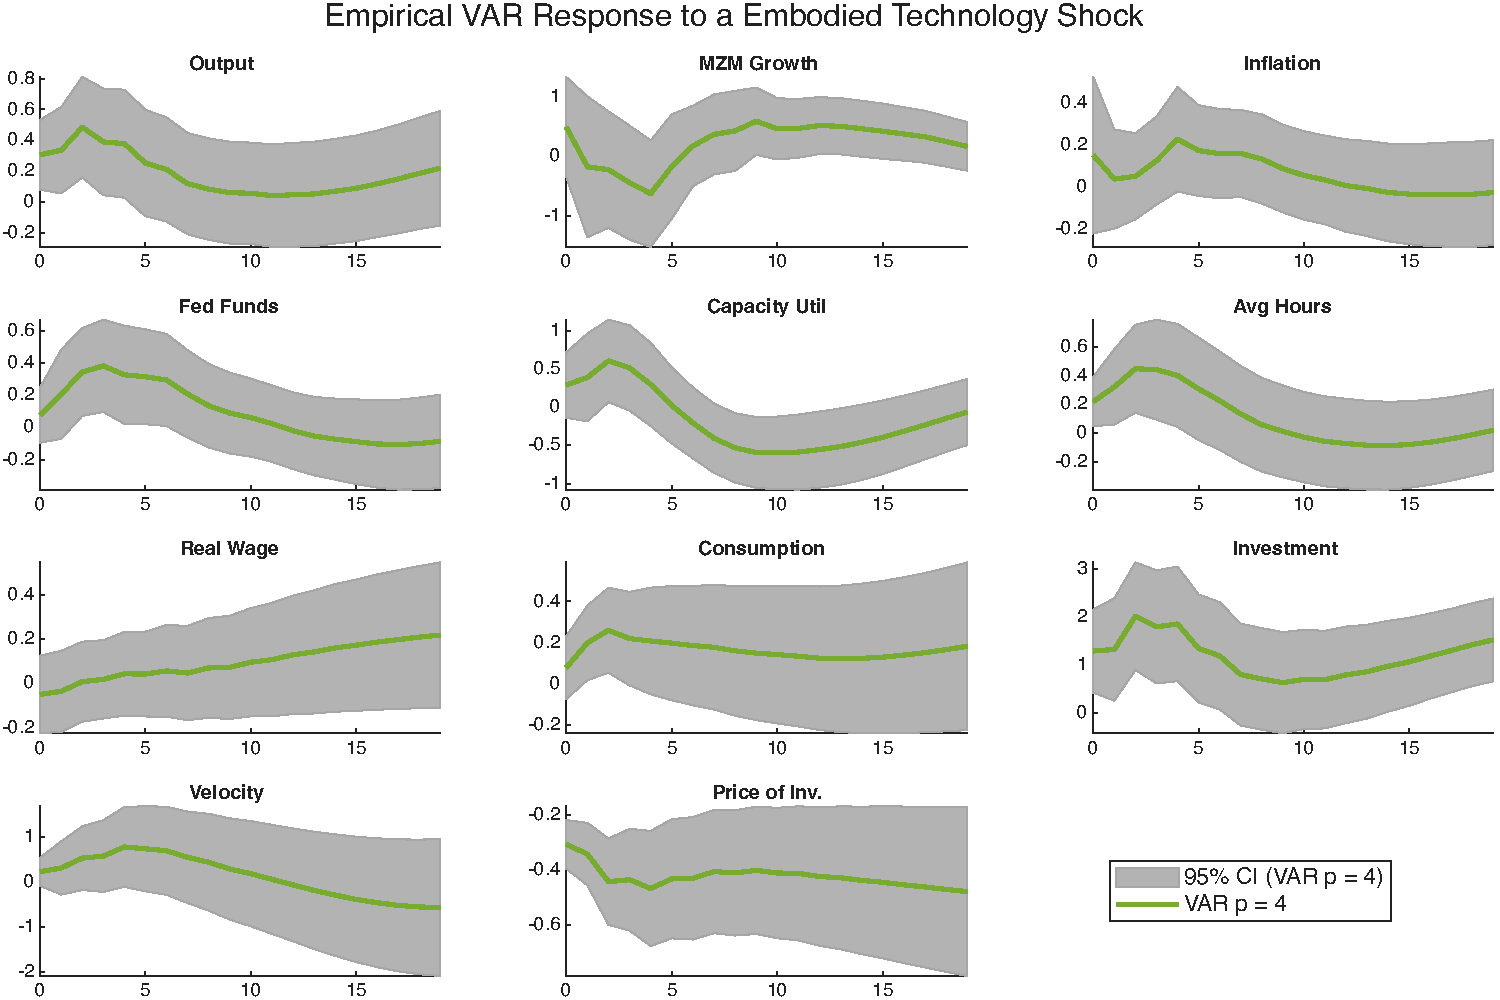
\includegraphics[width=1\linewidth]{../../Output/VAR_IRFs_Long_Lag_Progressively_Plots/Embodied_Technology_Shock/Step_1_UpToLag_4.pdf}}{\fbox{Image Path Broken or File Missing}}
    \caption{Embodied Technology Shock lag 4}
    \label{fig:VAR_et_baseline_lag4}
\end{figure}

\begin{figure}[htpb]
    \centering
    \IfFileExists{../../Output/VAR_IRFs_Long_Lag_Progressively_Plots/Embodied_Technology_Shock/Step_2_UpToLag_6.pdf}
    {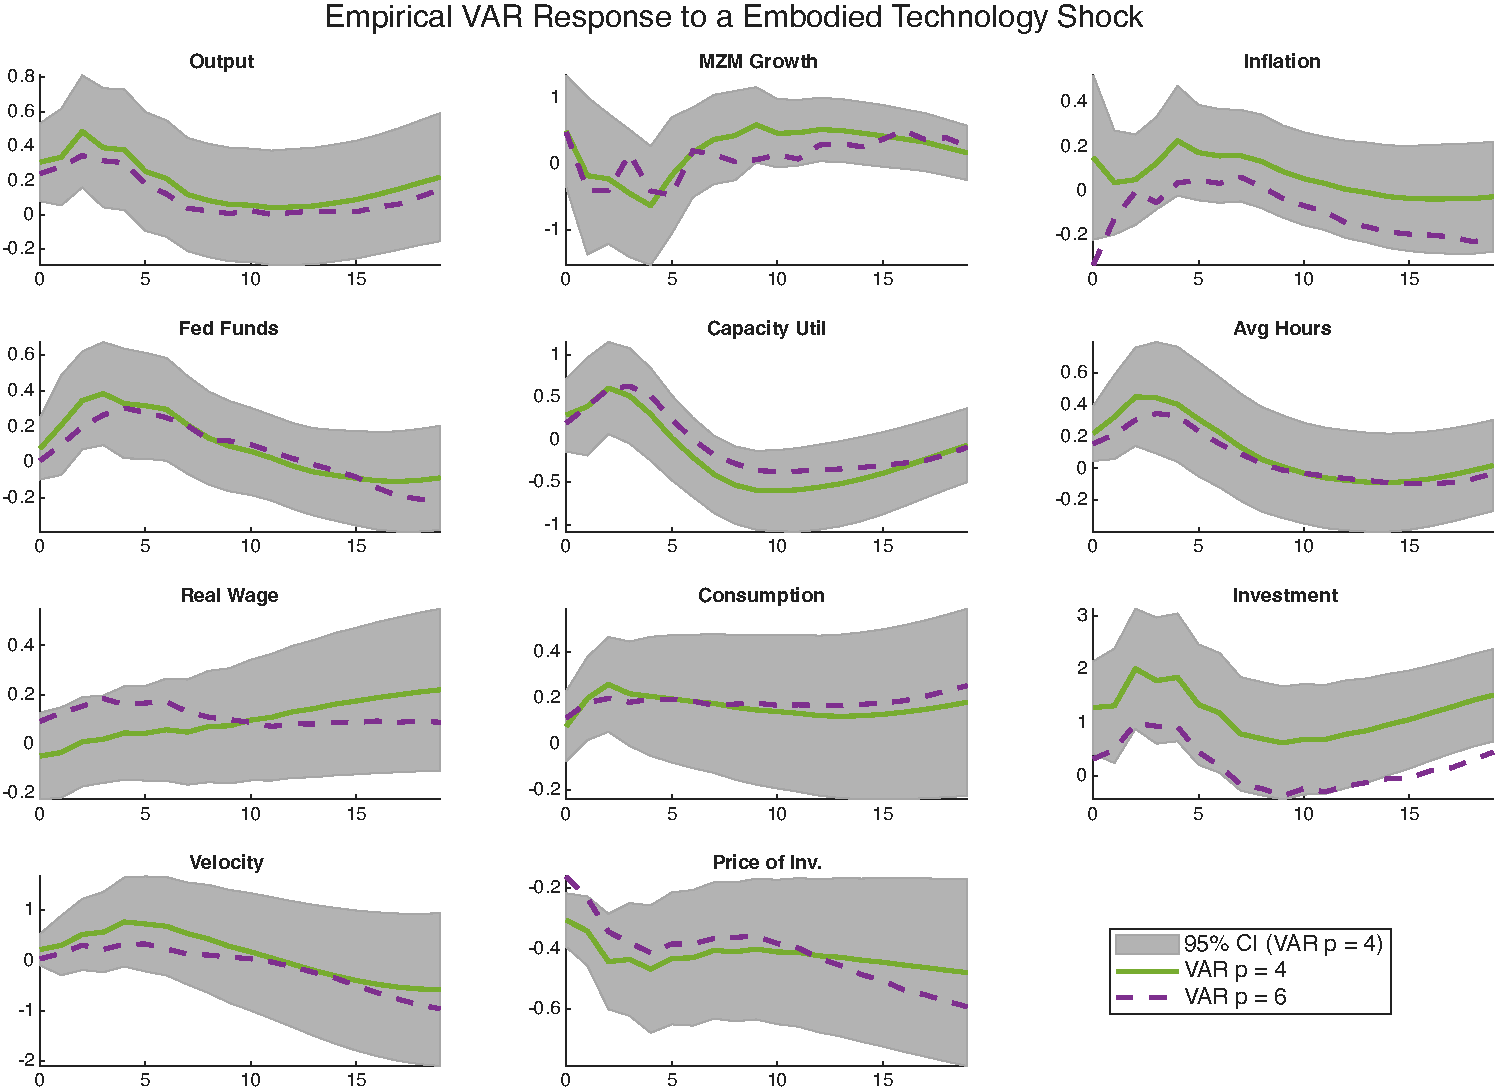
\includegraphics[width=1\linewidth]{../../Output/VAR_IRFs_Long_Lag_Progressively_Plots/Embodied_Technology_Shock/Step_2_UpToLag_6.pdf}}{\fbox{Image Path Broken or File Missing}}
    \caption{Embodied Technology Shock lag 6}
    \label{fig:VAR_et_baseline_lag6}
\end{figure}

\begin{figure}[htpb]
    \centering
    \IfFileExists{../../Output/VAR_IRFs_Long_Lag_Progressively_Plots/Embodied_Technology_Shock/Step_3_UpToLag_8.pdf}
    {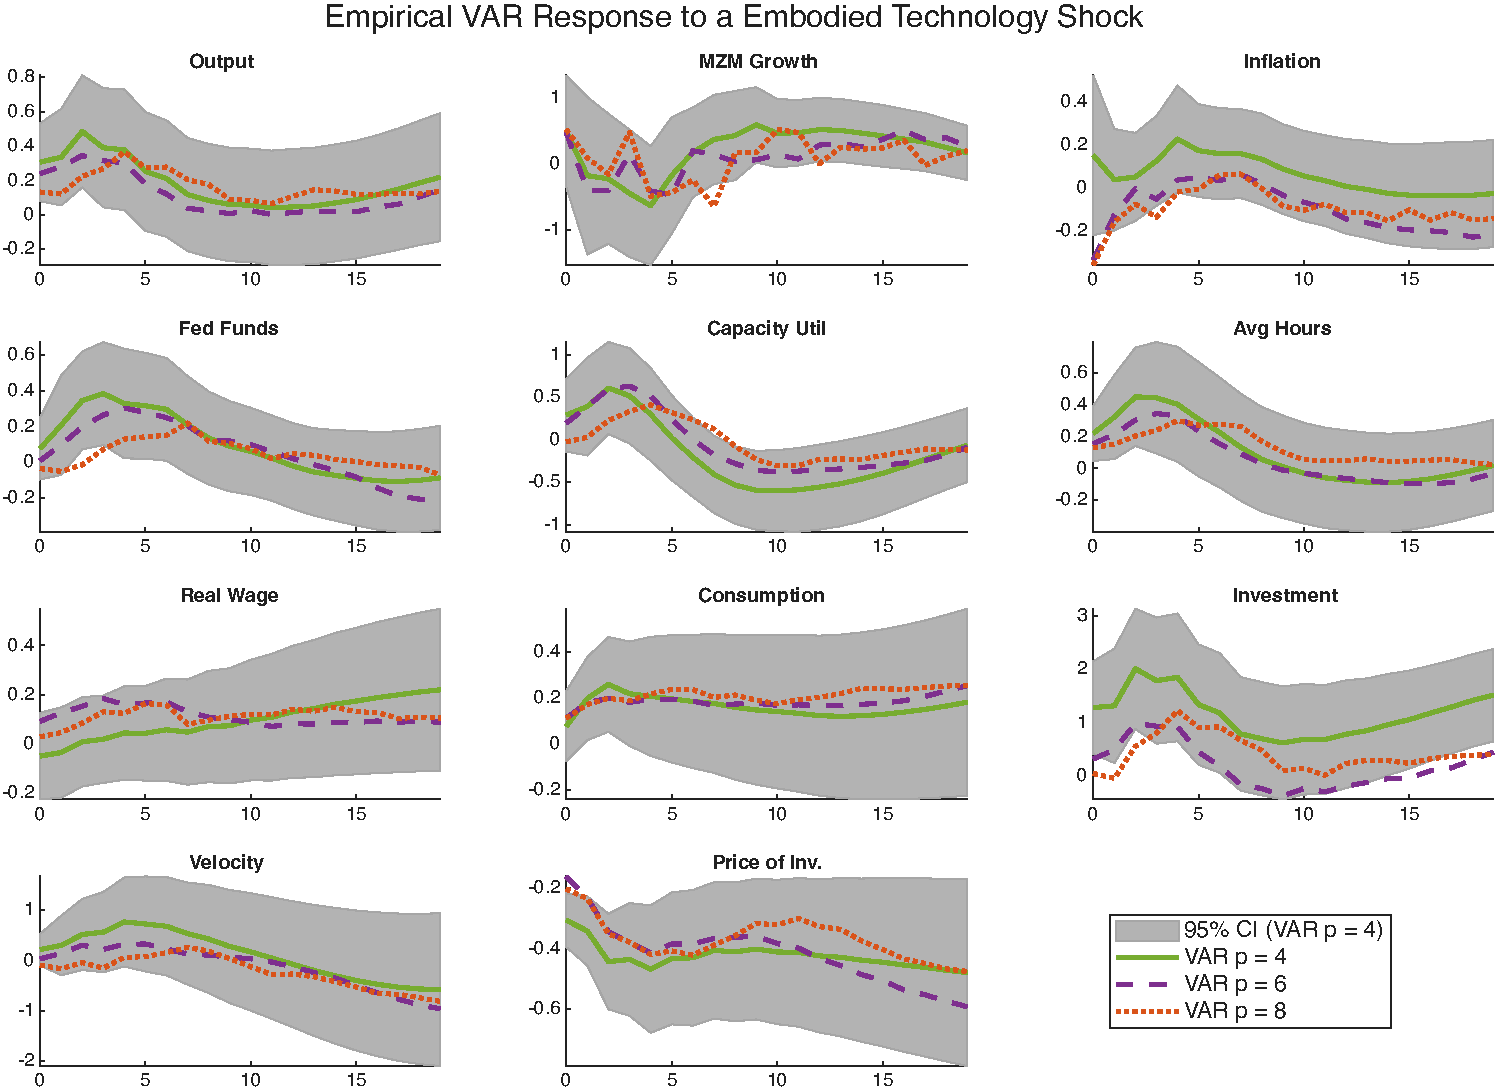
\includegraphics[width=1\linewidth]{../../Output/VAR_IRFs_Long_Lag_Progressively_Plots/Embodied_Technology_Shock/Step_3_UpToLag_8.pdf}}{\fbox{Image Path Broken or File Missing}}
    \caption{Embodied Technology Shock lag 8}
    \label{fig:VAR_et_baseline_lag8}
\end{figure}

\begin{figure}[htpb]
    \centering
    \IfFileExists{../../Output/VAR_IRFs_Long_Lag_Progressively_Plots/Embodied_Technology_Shock/Step_4_UpToLag_10.pdf}
    {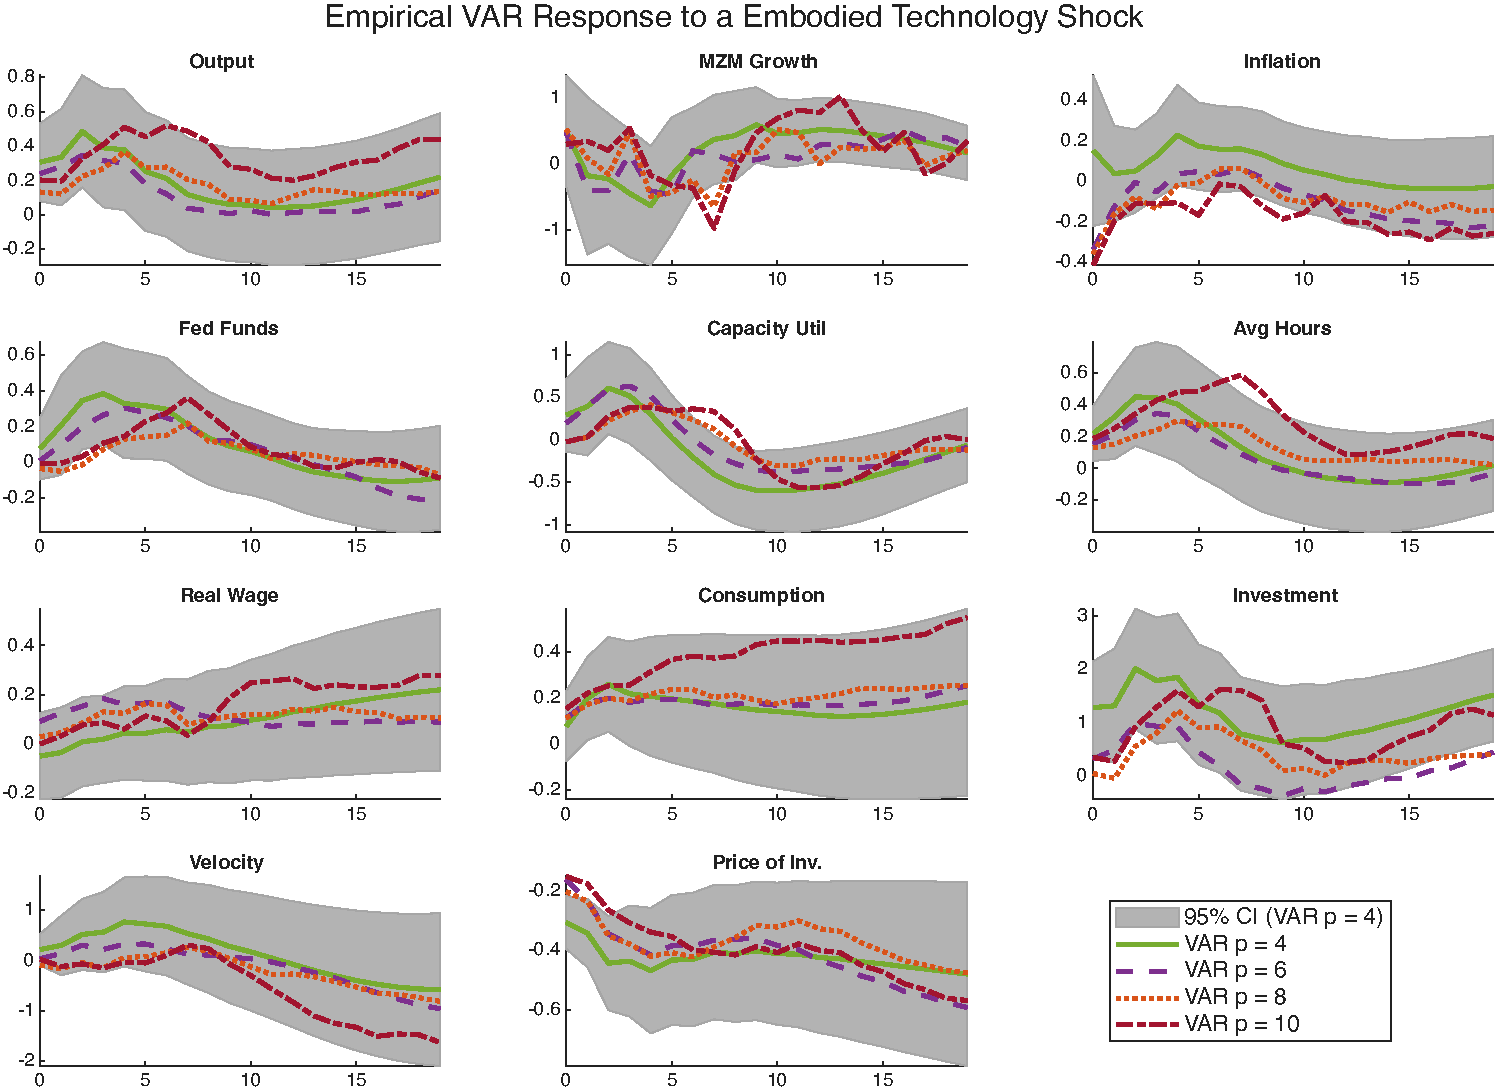
\includegraphics[width=1\linewidth]{../../Output/VAR_IRFs_Long_Lag_Progressively_Plots/Embodied_Technology_Shock/Step_4_UpToLag_10.pdf}}{\fbox{Image Path Broken or File Missing}}
    \caption{Embodied Technology Shock lag 10}
    \label{fig:VAR_et_baseline_lag10}
\end{figure}

\begin{figure}[htpb]
    \centering
    \IfFileExists{../../Output/VAR_IRFs_Long_Lag_Progressively_Plots/Embodied_Technology_Shock/Step_5_UpToLag_12.pdf}
    {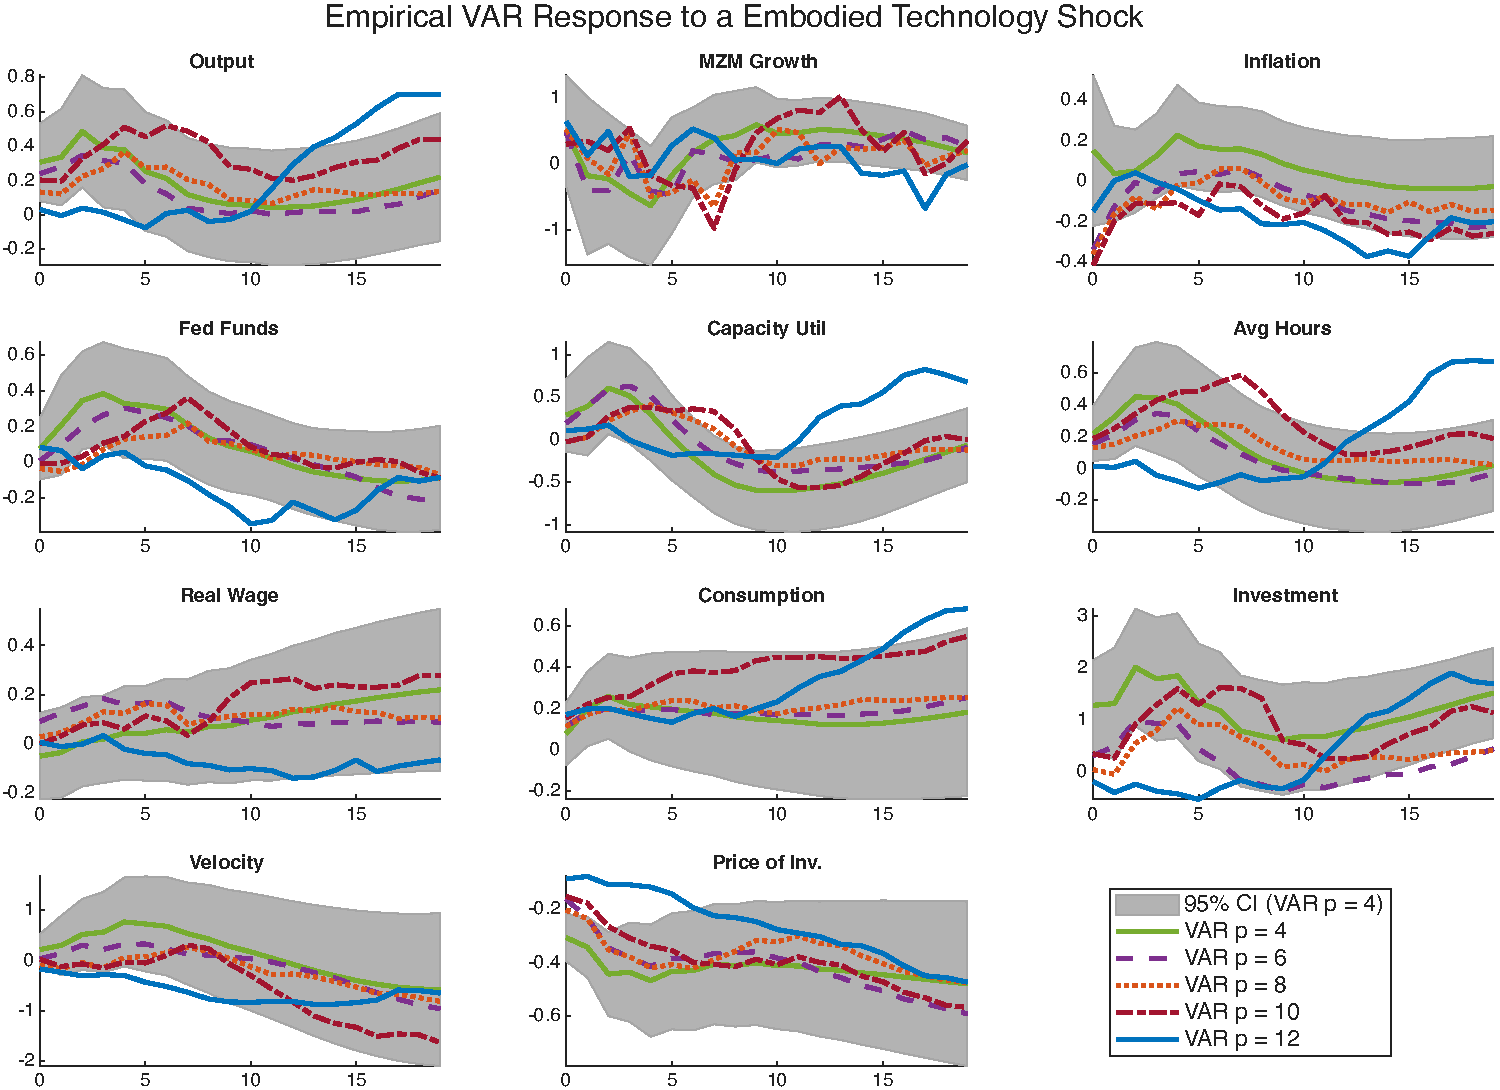
\includegraphics[width=1\linewidth]{../../Output/VAR_IRFs_Long_Lag_Progressively_Plots/Embodied_Technology_Shock/Step_5_UpToLag_12.pdf}}{\fbox{Image Path Broken or File Missing}}
    \caption{Embodied Technology Shock lag 12}
    \label{fig:VAR_et_baseline_lag12}
\end{figure}

\FloatBarrier
\subsection{ACEL 2005 VAR Across different lag structures Progressively Comparison: Neutral Technology Shock}

\begin{figure}[htpb]
    \centering
    \IfFileExists{../../Output/VAR_IRFs_Long_Lag_Progressively_Plots/Neutral_Technology_Shock/Step_1_UpToLag_4.pdf}
    {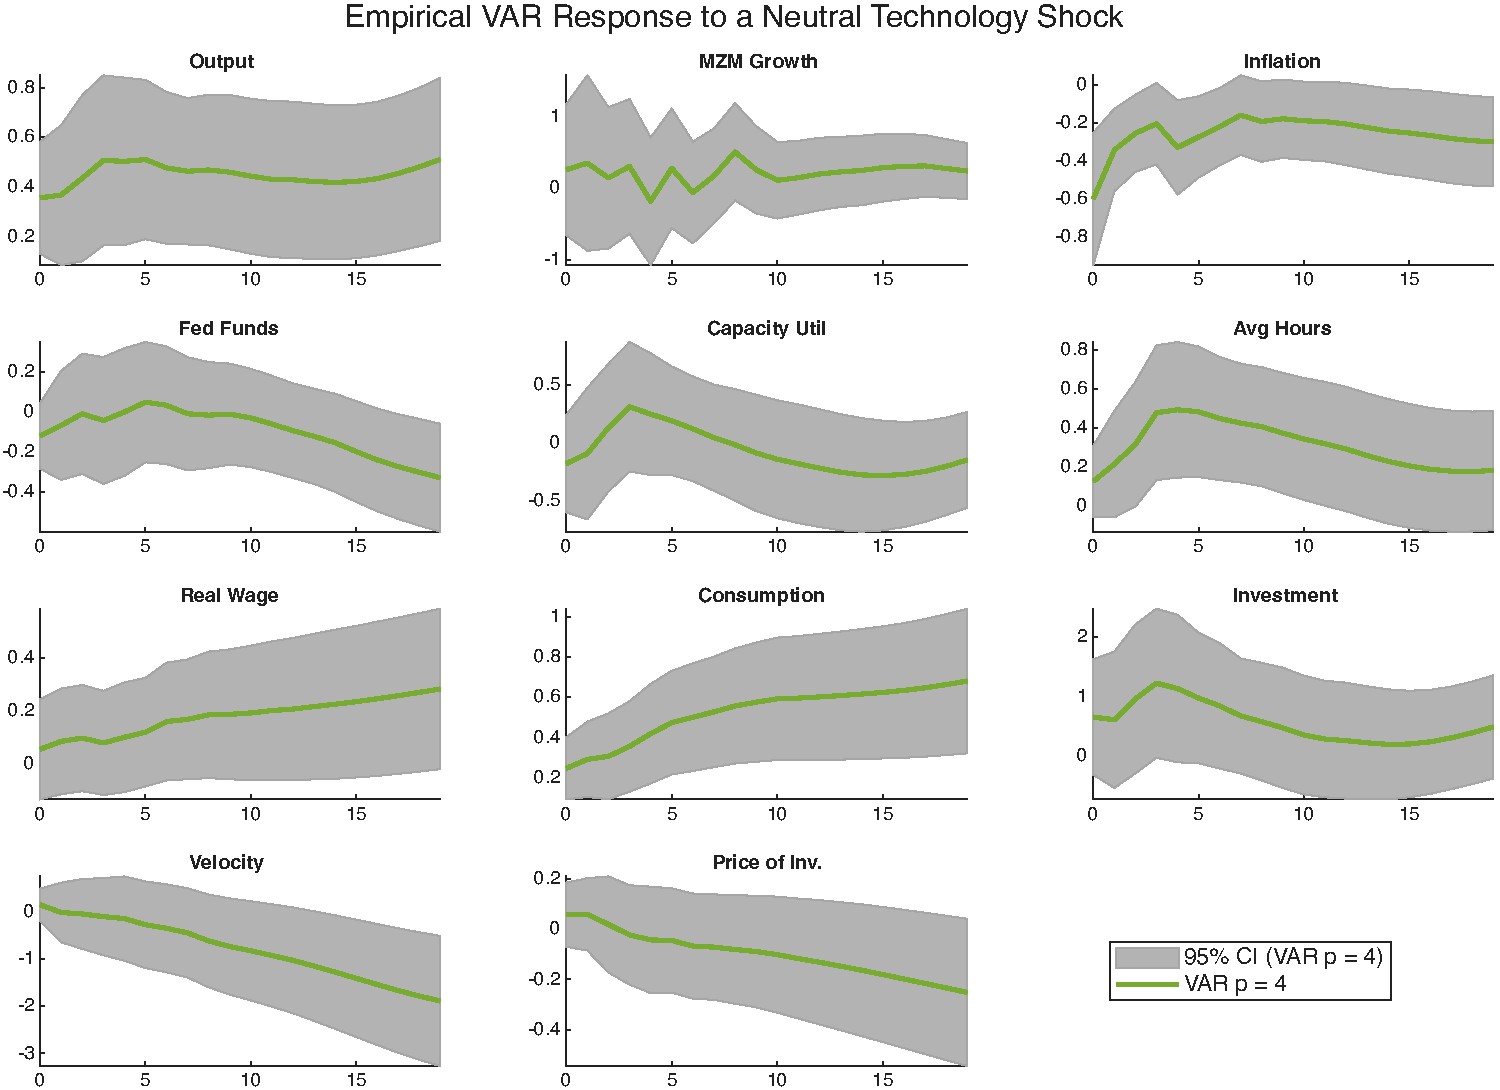
\includegraphics[width=1\linewidth]{../../Output/VAR_IRFs_Long_Lag_Progressively_Plots/Neutral_Technology_Shock/Step_1_UpToLag_4.pdf}}{\fbox{Image Path Broken or File Missing}}
    \caption{Neutral Technology Shock lag 4}
    \label{fig:VAR_nt_baseline_lag4}
\end{figure}

\begin{figure}[htpb]
    \centering
    \IfFileExists{../../Output/VAR_IRFs_Long_Lag_Progressively_Plots/Neutral_Technology_Shock/Step_2_UpToLag_6.pdf}
    {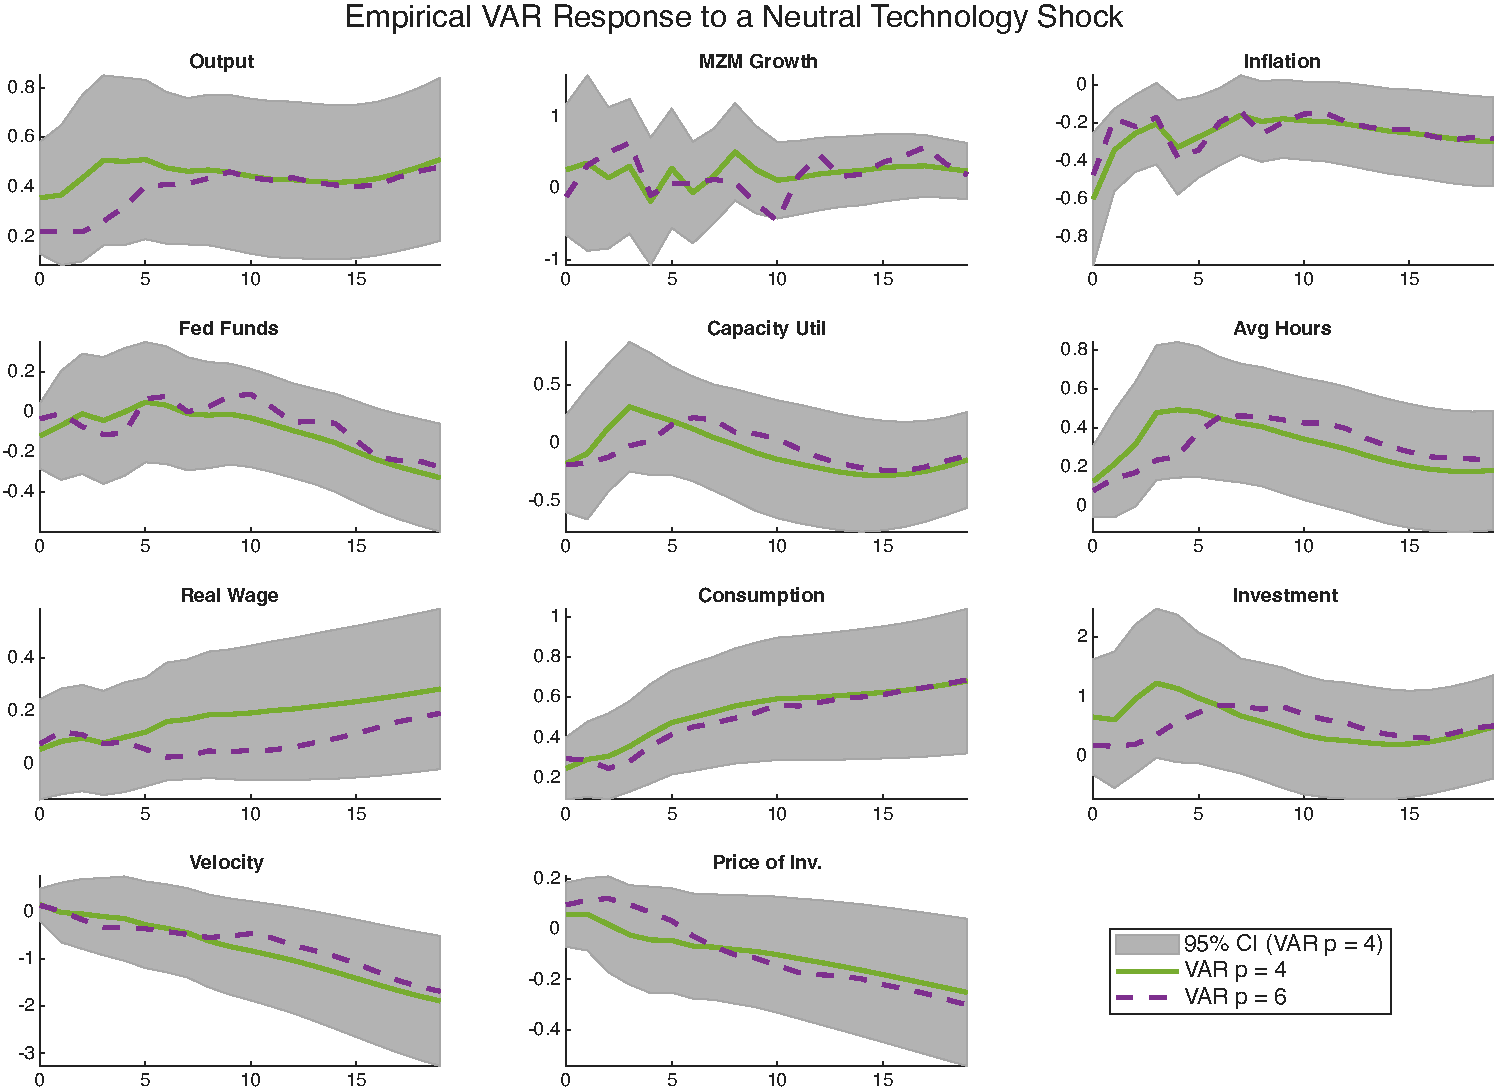
\includegraphics[width=1\linewidth]{../../Output/VAR_IRFs_Long_Lag_Progressively_Plots/Neutral_Technology_Shock/Step_2_UpToLag_6.pdf}}{\fbox{Image Path Broken or File Missing}}
    \caption{Neutral Technology Shock lag 6}
    \label{fig:VAR_nt_baseline_lag6}
\end{figure}

\begin{figure}[htpb]
    \centering
    \IfFileExists{../../Output/VAR_IRFs_Long_Lag_Progressively_Plots/Neutral_Technology_Shock/Step_3_UpToLag_8.pdf}
    {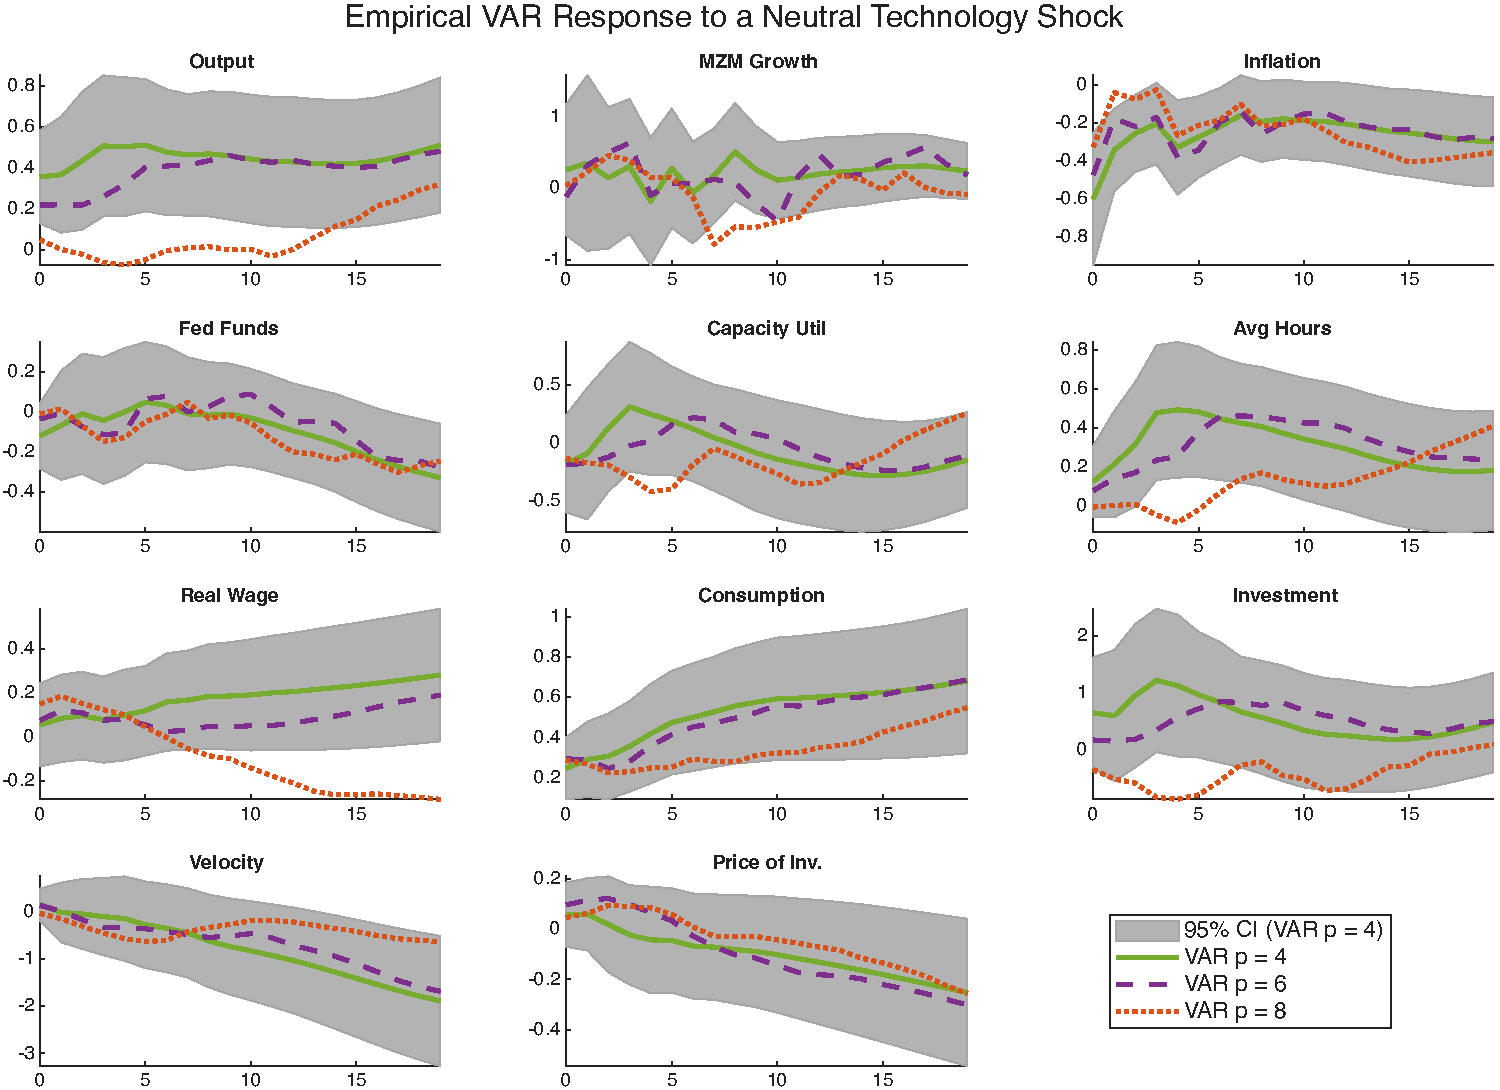
\includegraphics[width=1\linewidth]{../../Output/VAR_IRFs_Long_Lag_Progressively_Plots/Neutral_Technology_Shock/Step_3_UpToLag_8.pdf}}{\fbox{Image Path Broken or File Missing}}
    \caption{Neutral Technology Shock lag 8}
    \label{fig:VAR_nt_baseline_lag8}
\end{figure}

\begin{figure}[htpb]
    \centering
    \IfFileExists{../../Output/VAR_IRFs_Long_Lag_Progressively_Plots/Neutral_Technology_Shock/Step_4_UpToLag_10.pdf}
    {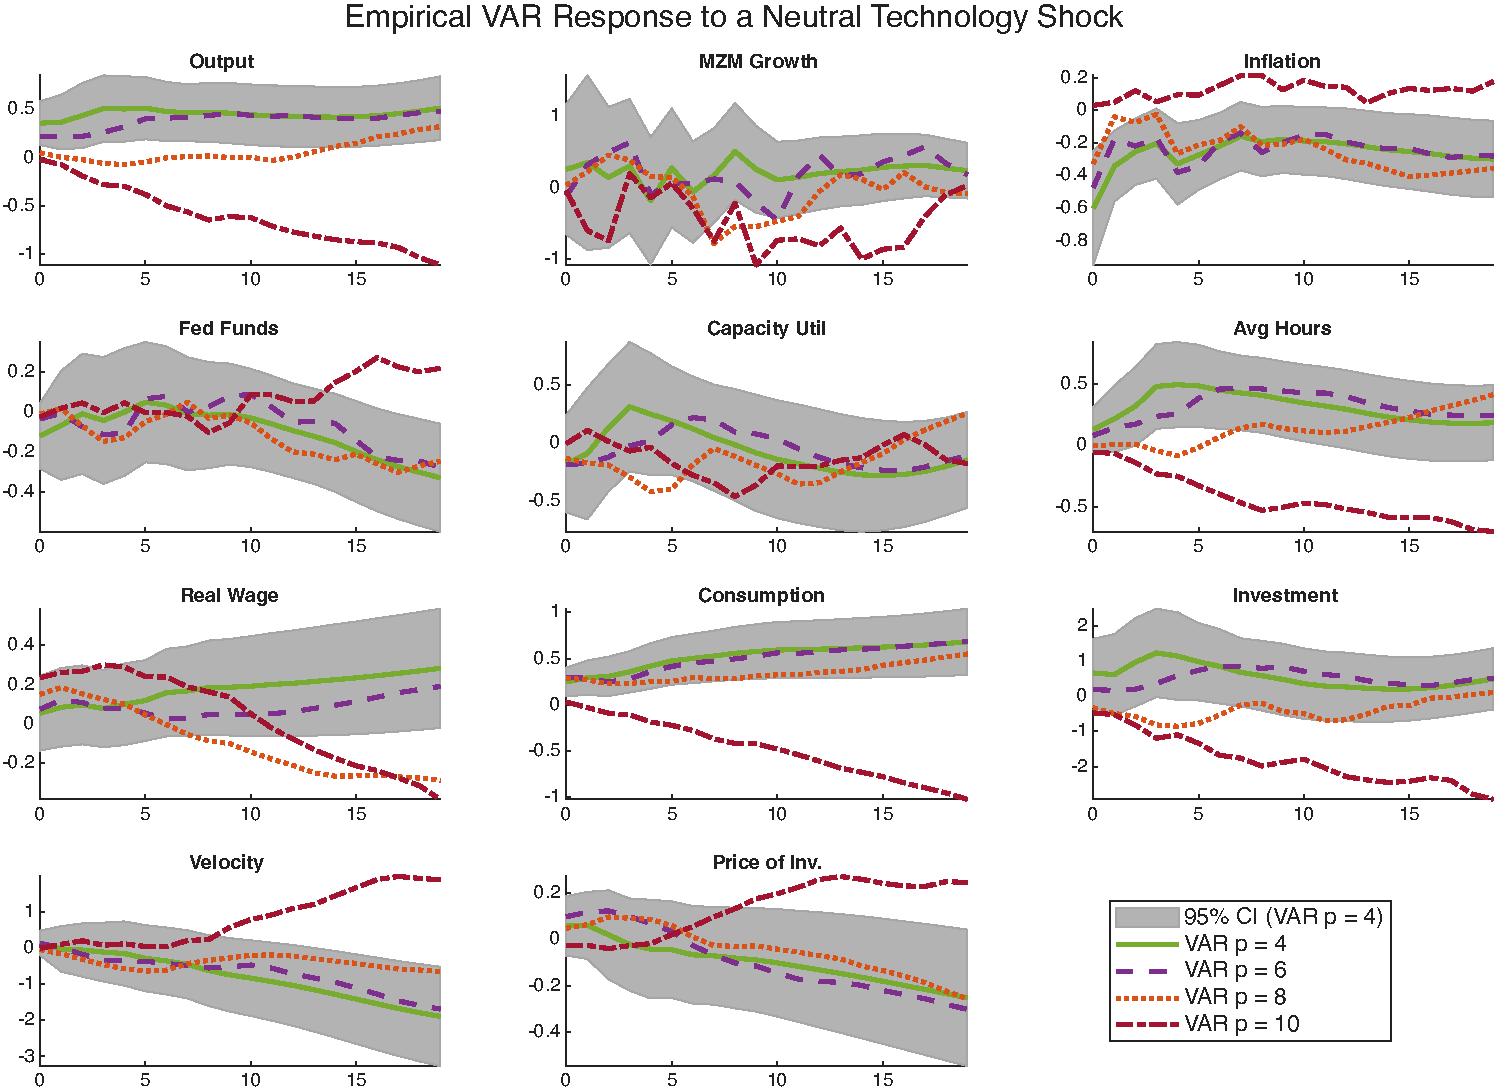
\includegraphics[width=1\linewidth]{../../Output/VAR_IRFs_Long_Lag_Progressively_Plots/Neutral_Technology_Shock/Step_4_UpToLag_10.pdf}}{\fbox{Image Path Broken or File Missing}}
    \caption{Neutral Technology Shock lag 10}
    \label{fig:VAR_nt_baseline_lag10}
\end{figure}

\begin{figure}[htpb]
    \centering
    \IfFileExists{../../Output/VAR_IRFs_Long_Lag_Progressively_Plots/Neutral_Technology_Shock/Step_5_UpToLag_12.pdf}
    {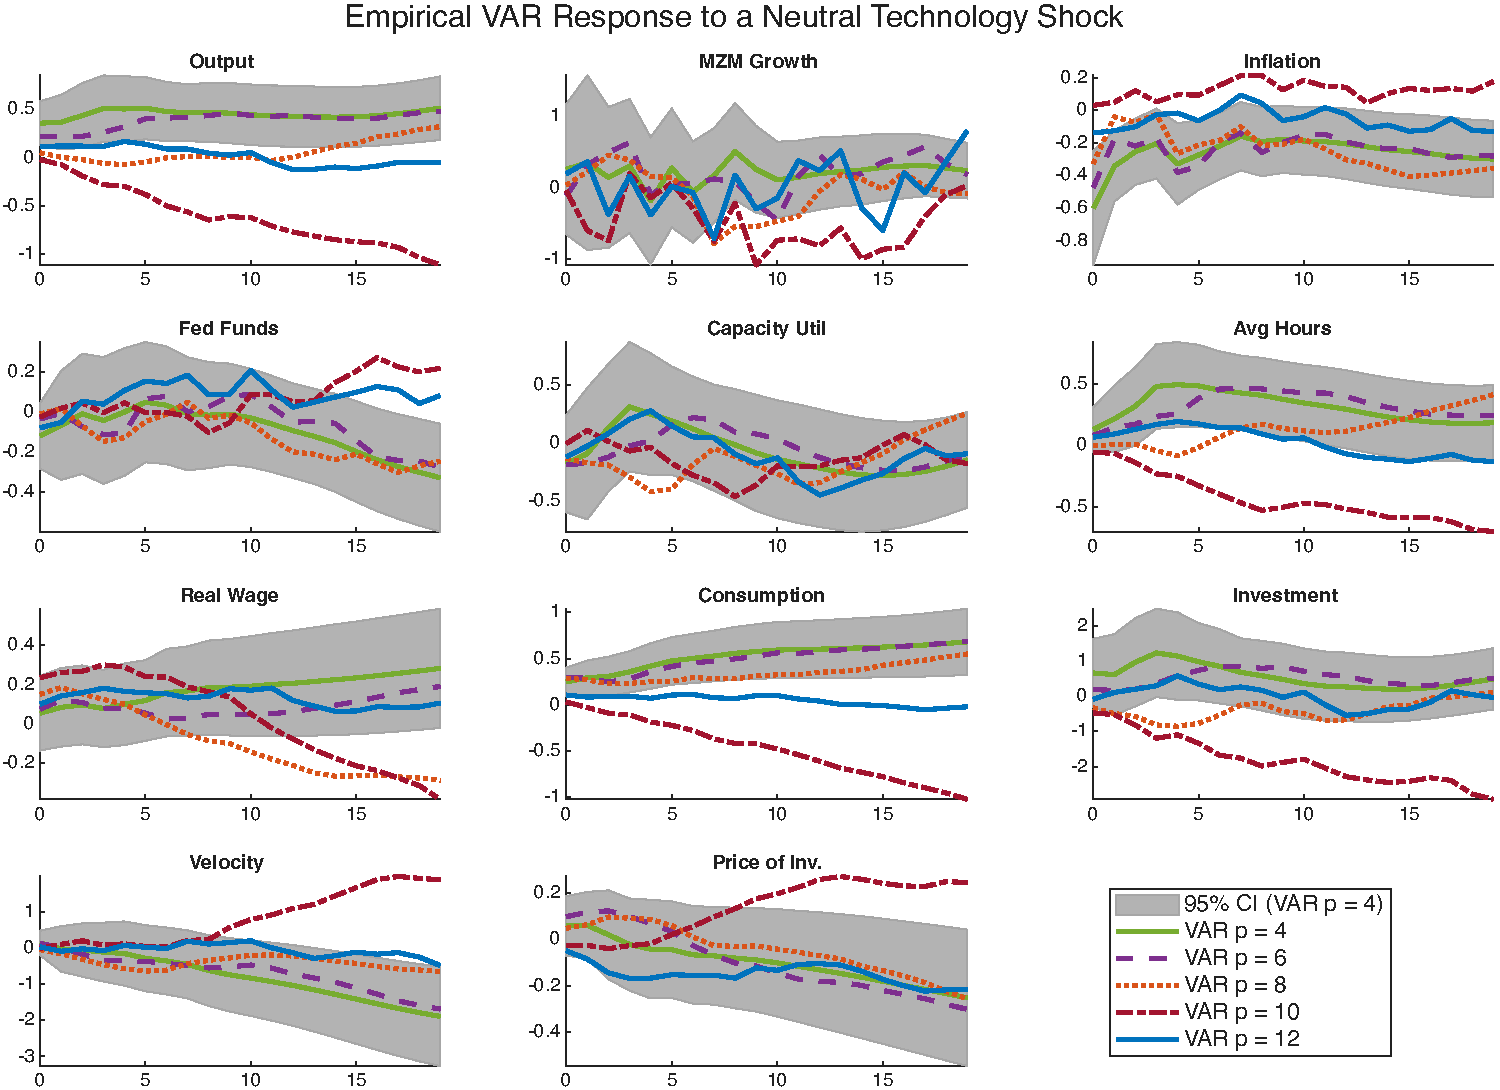
\includegraphics[width=1\linewidth]{../../Output/VAR_IRFs_Long_Lag_Progressively_Plots/Neutral_Technology_Shock/Step_5_UpToLag_12.pdf}}{\fbox{Image Path Broken or File Missing}}
    \caption{Neutral Technology Shock lag 12}
    \label{fig:VAR_nt_baseline_lag12}
\end{figure}

\FloatBarrier

\subsection{ACEL 2005 DSGE Across different lag structures Progressively Comparison: Monetary Policy Shock}

\begin{figure}[htpb]
    \centering
    \IfFileExists{../../Output/DSGE_IRFs_Long_Lag_Progressively_Plots/Monetary_Policy_Shock/Step_1_UpToLag_4.pdf}
    {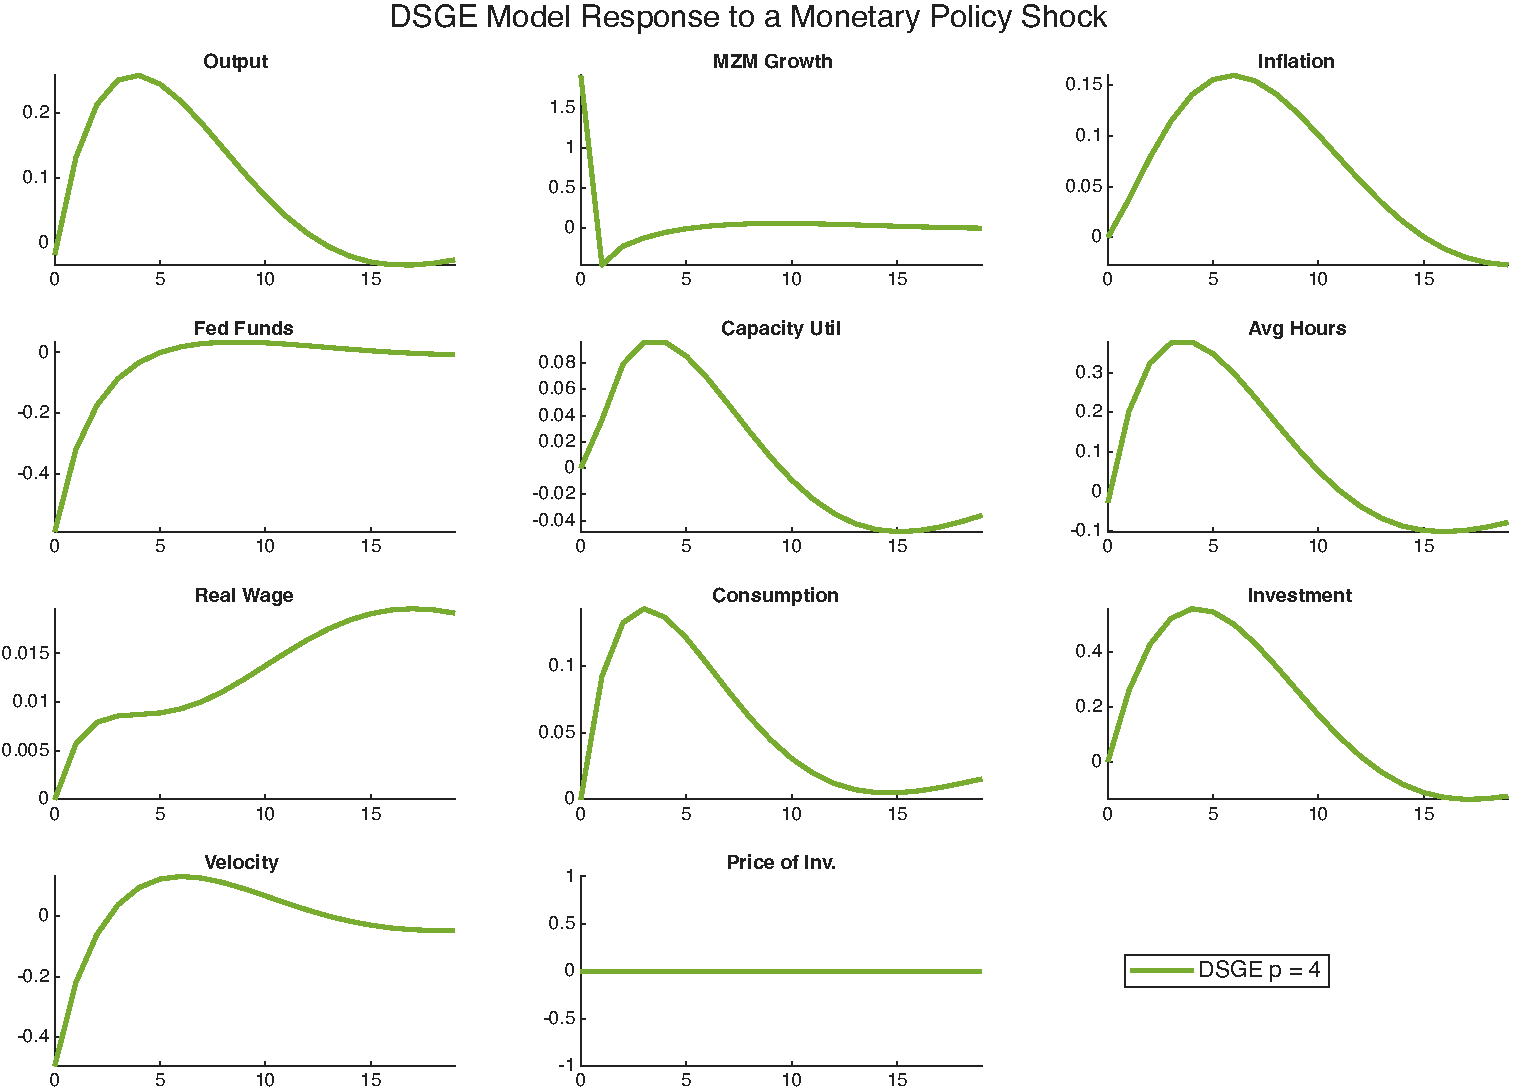
\includegraphics[width=1\linewidth]{../../Output/DSGE_IRFs_Long_Lag_Progressively_Plots/Monetary_Policy_Shock/Step_1_UpToLag_4.pdf}}{\fbox{Image Path Broken or File Missing}}
    \caption{DSGE Monetary Policy Shock lag 4}
    \label{fig:DSGE_mp_baseline_lag4}
\end{figure}

\begin{figure}[htpb]
    \centering
    \IfFileExists{../../Output/DSGE_IRFs_Long_Lag_Progressively_Plots/Monetary_Policy_Shock/Step_2_UpToLag_6.pdf}
    {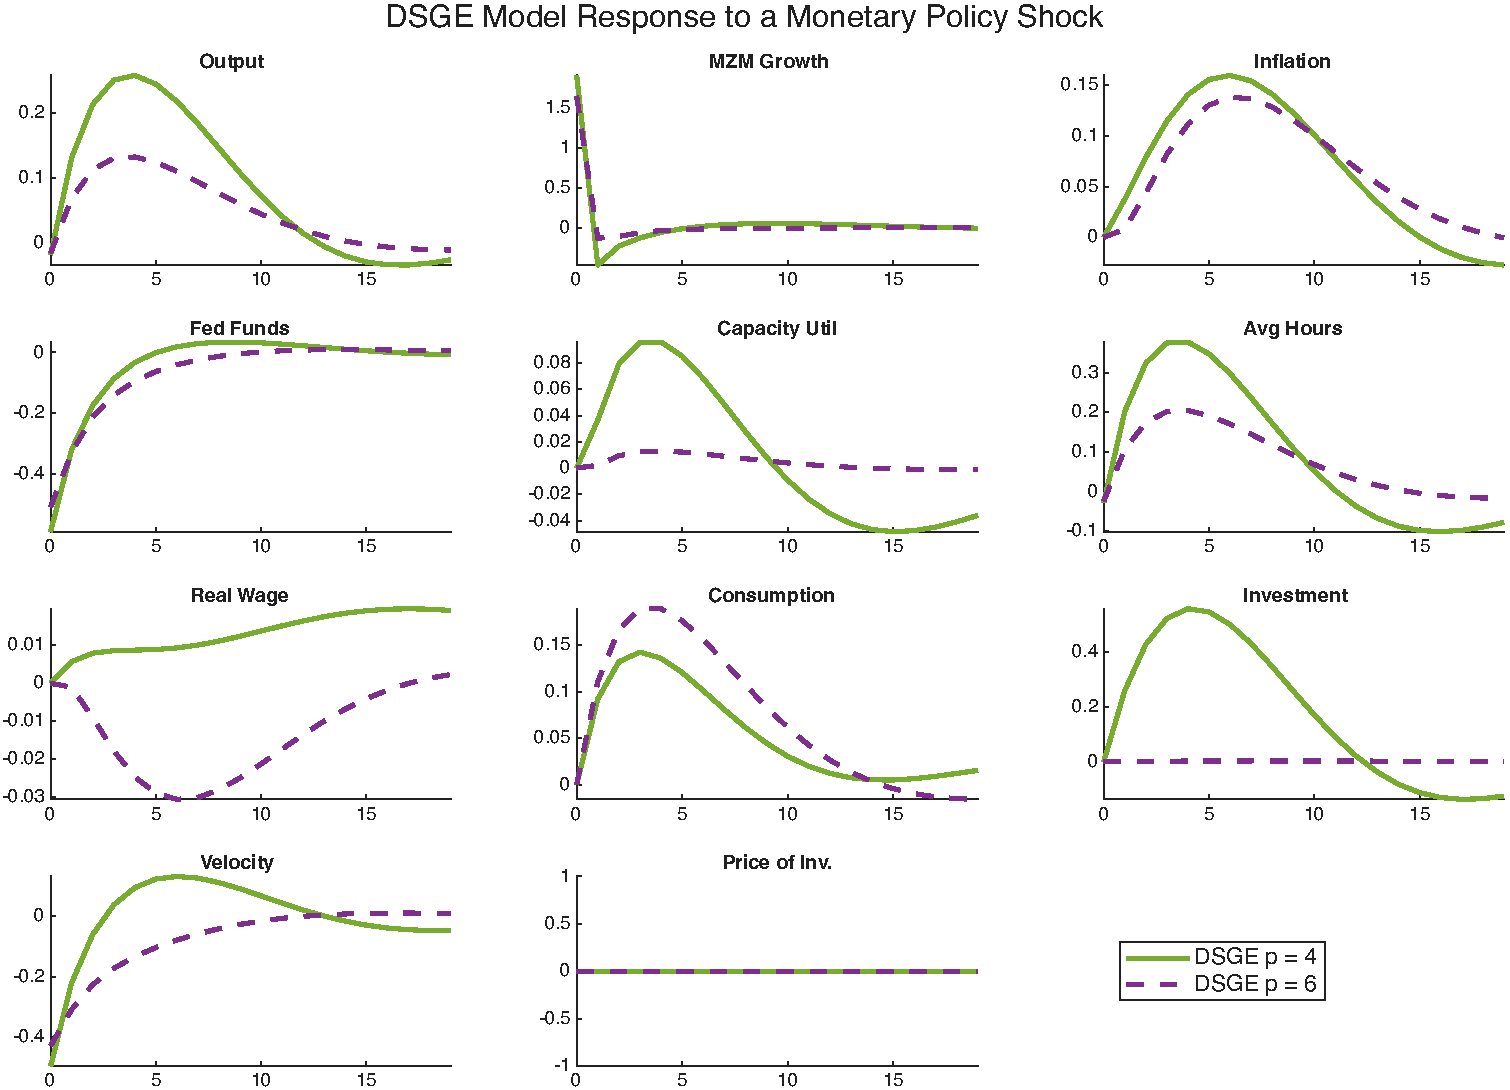
\includegraphics[width=1\linewidth]{../../Output/DSGE_IRFs_Long_Lag_Progressively_Plots/Monetary_Policy_Shock/Step_2_UpToLag_6.pdf}}{\fbox{Image Path Broken or File Missing}}
    \caption{DSGE Monetary Policy Shock lag 6}
    \label{fig:DSGE_mp_baseline_lag6}
\end{figure}

\begin{figure}[htpb]
    \centering
    \IfFileExists{../../Output/DSGE_IRFs_Long_Lag_Progressively_Plots/Monetary_Policy_Shock/Step_3_UpToLag_8.pdf}
    {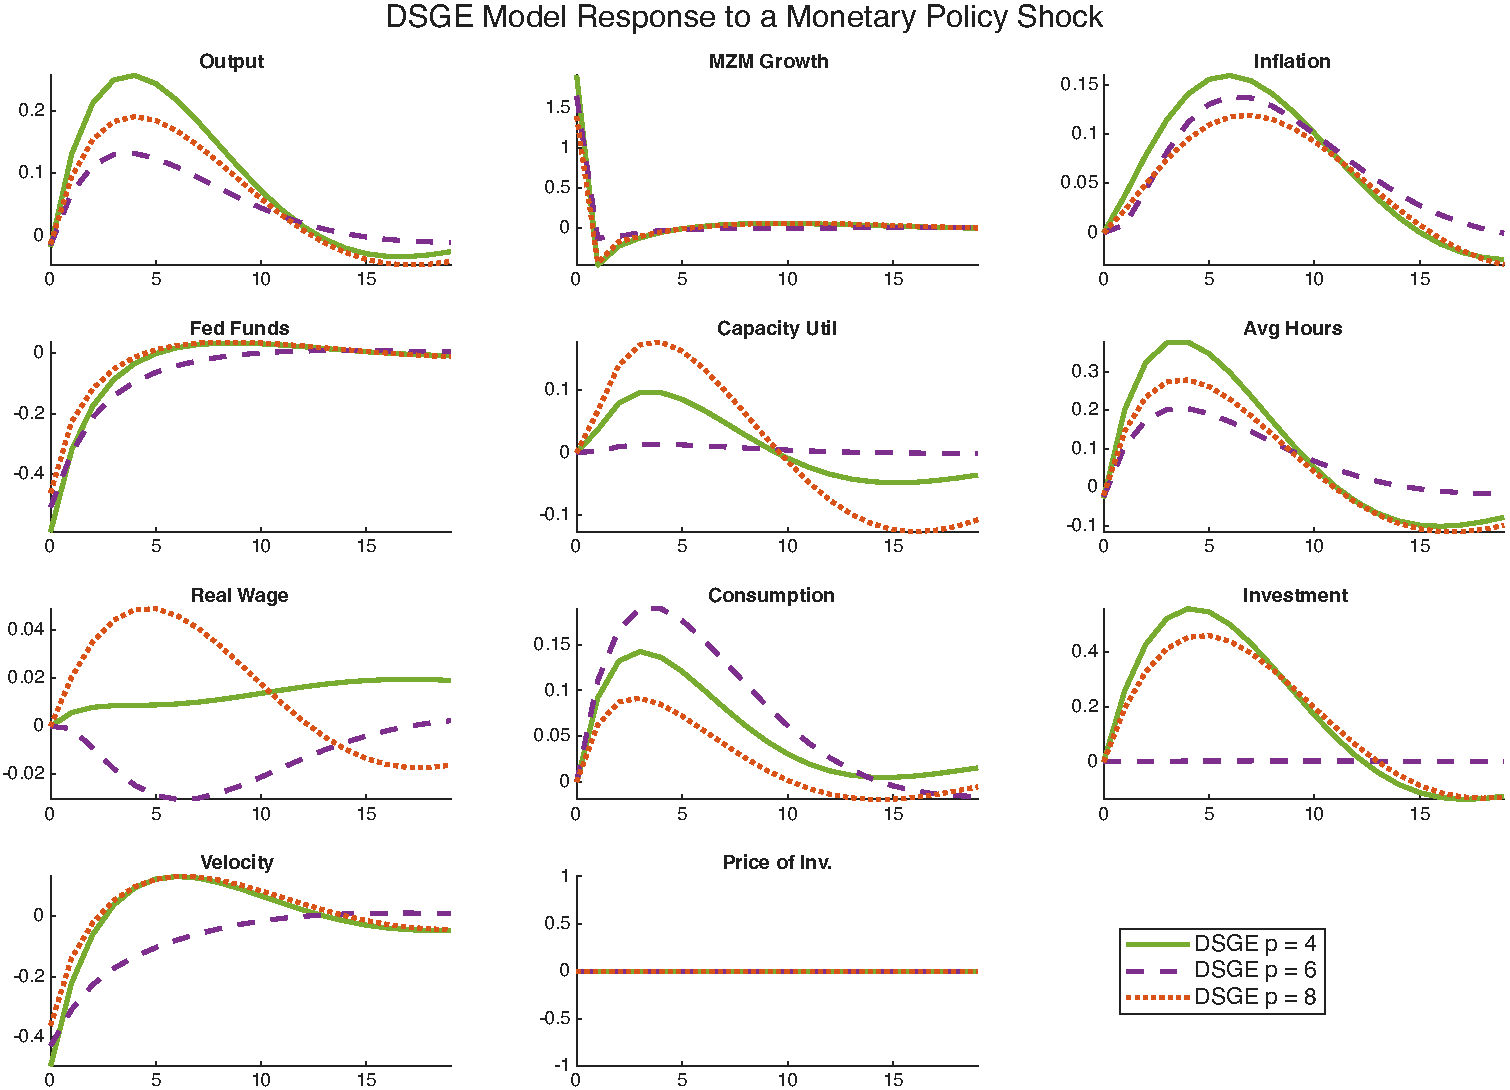
\includegraphics[width=1\linewidth]{../../Output/DSGE_IRFs_Long_Lag_Progressively_Plots/Monetary_Policy_Shock/Step_3_UpToLag_8.pdf}}{\fbox{Image Path Broken or File Missing}}
    \caption{DSGE Monetary Policy Shock lag 8}
    \label{fig:DSGE_mp_baseline_lag8}
\end{figure}

\begin{figure}[htpb]
    \centering
    \IfFileExists{../../Output/DSGE_IRFs_Long_Lag_Progressively_Plots/Monetary_Policy_Shock/Step_4_UpToLag_10.pdf}
    {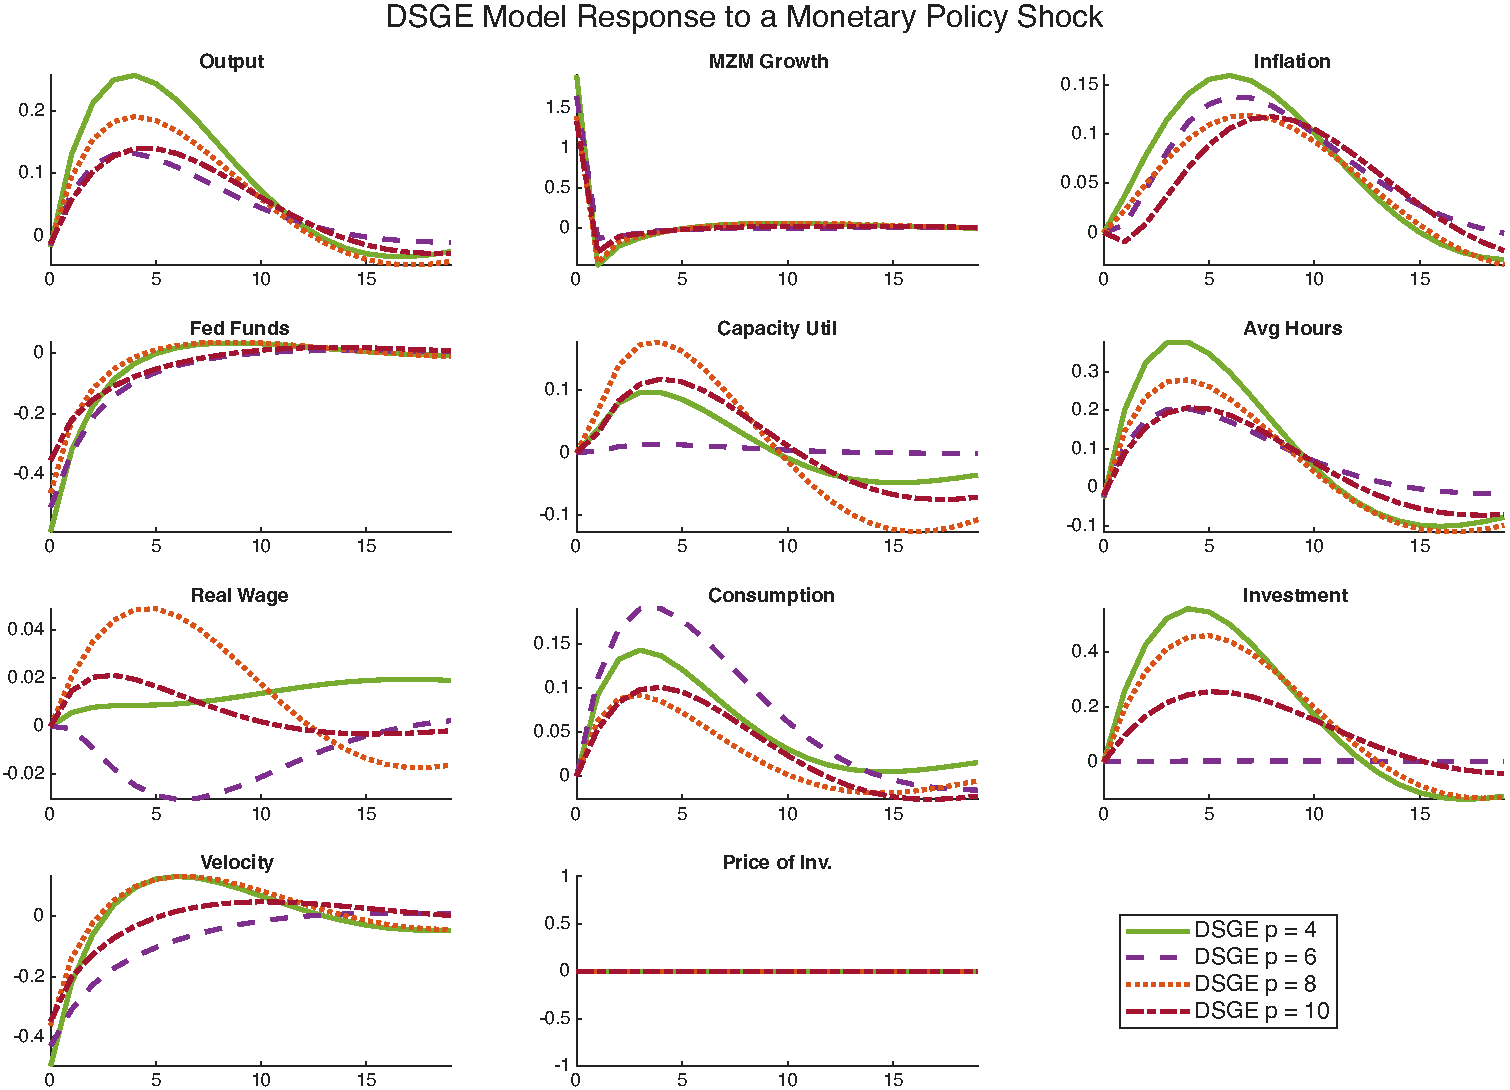
\includegraphics[width=1\linewidth]{../../Output/DSGE_IRFs_Long_Lag_Progressively_Plots/Monetary_Policy_Shock/Step_4_UpToLag_10.pdf}}{\fbox{Image Path Broken or File Missing}}
    \caption{DSGE Monetary Policy Shock lag 10}
    \label{fig:DSGE_mp_baseline_lag10}
\end{figure}

\begin{figure}[htpb]
    \centering
    \IfFileExists{../../Output/DSGE_IRFs_Long_Lag_Progressively_Plots/Monetary_Policy_Shock/Step_5_UpToLag_12.pdf}
    {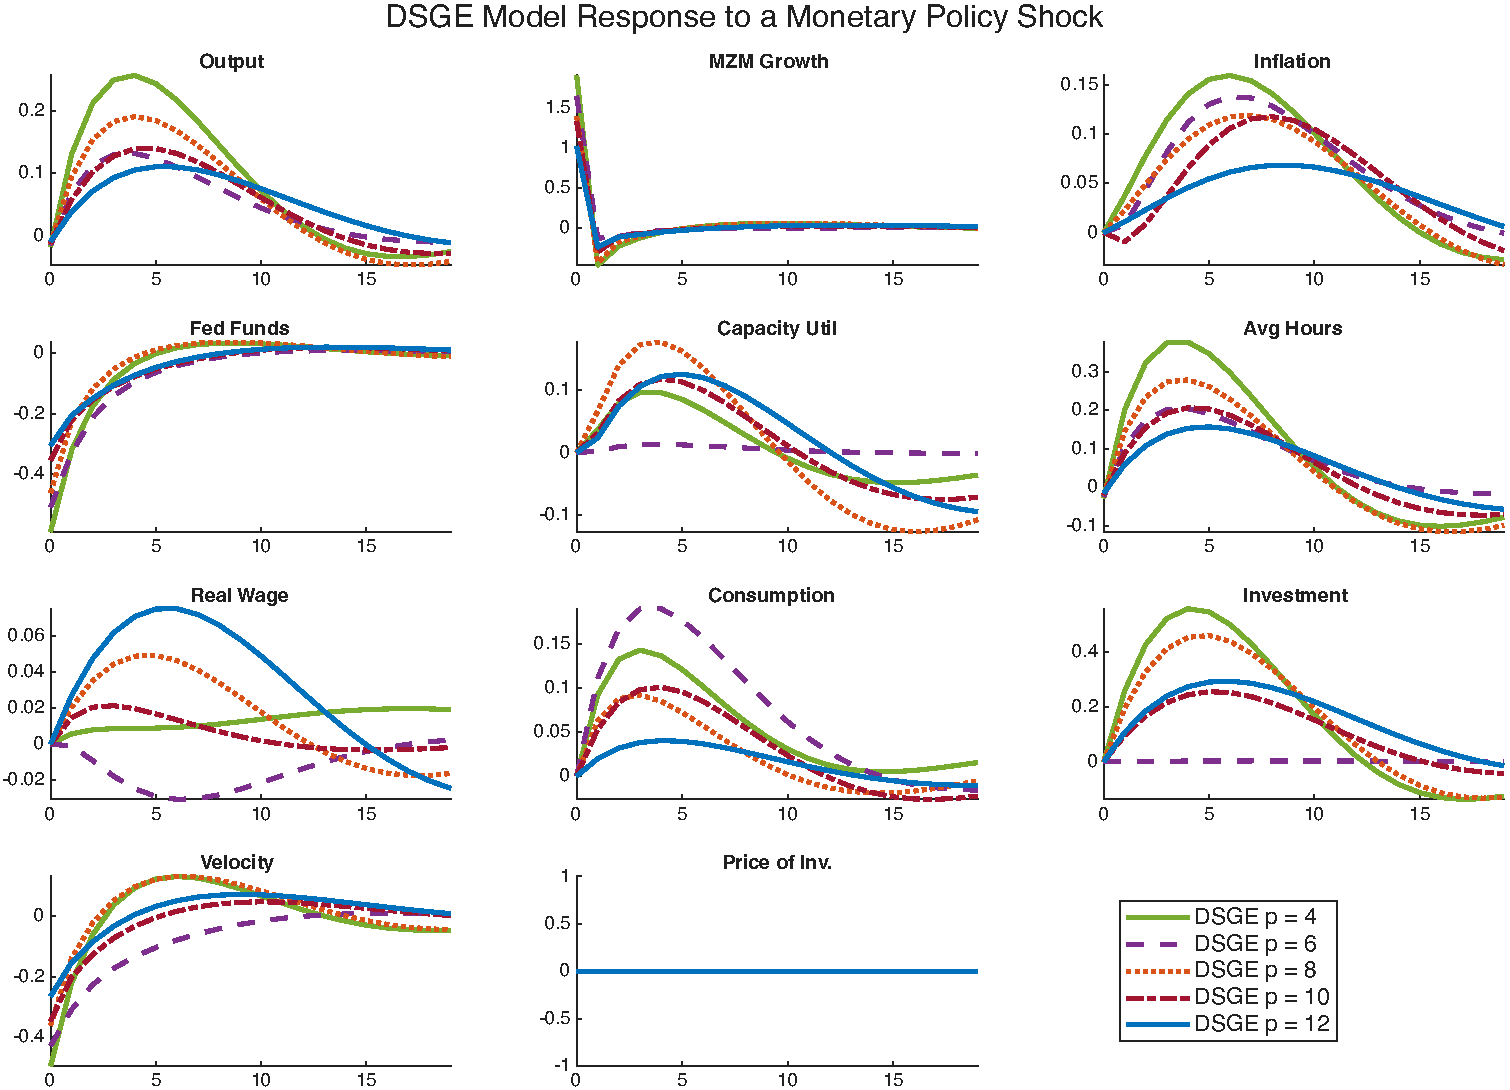
\includegraphics[width=1\linewidth]{../../Output/DSGE_IRFs_Long_Lag_Progressively_Plots/Monetary_Policy_Shock/Step_5_UpToLag_12.pdf}}{\fbox{Image Path Broken or File Missing}}
    \caption{DSGE Monetary Policy Shock lag 12}
    \label{fig:DSGE_mp_baseline_lag12}
\end{figure}

\FloatBarrier
\subsection{ACEL 2005 DSGE Across different lag structures Progressively Comparison: Embodied Technology Shock}

\begin{figure}[htpb]
    \centering
    \IfFileExists{../../Output/DSGE_IRFs_Long_Lag_Progressively_Plots/Embodied_Technology_Shock/Step_1_UpToLag_4.pdf}
    {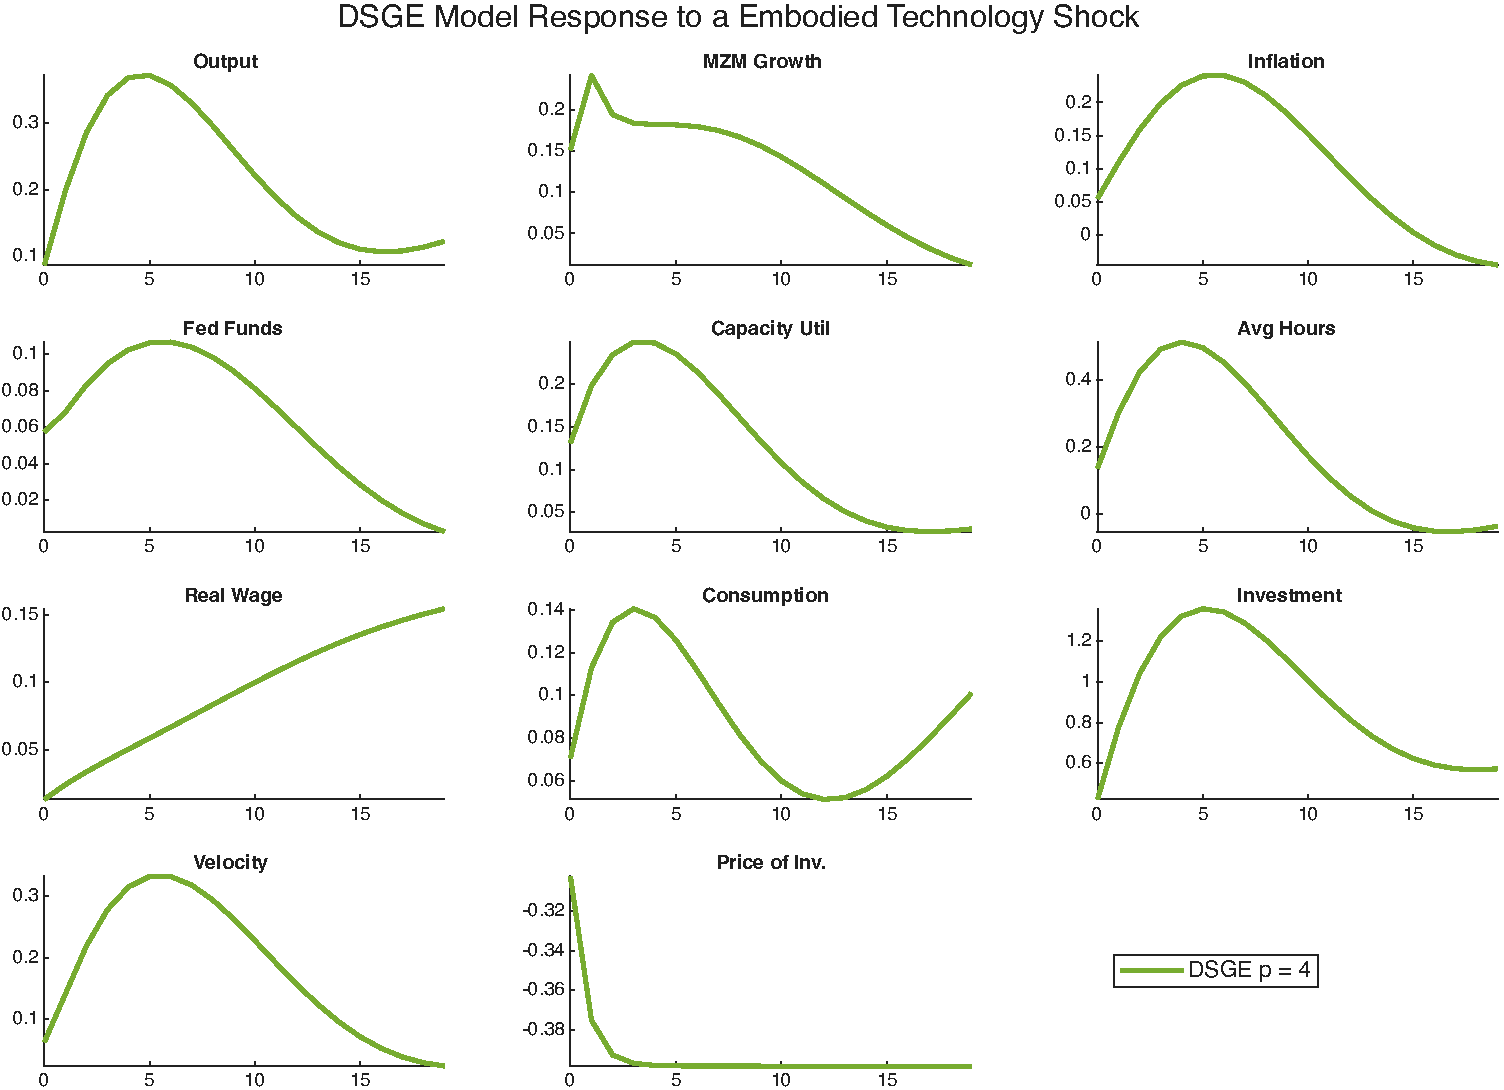
\includegraphics[width=1\linewidth]{../../Output/DSGE_IRFs_Long_Lag_Progressively_Plots/Embodied_Technology_Shock/Step_1_UpToLag_4.pdf}}{\fbox{Image Path Broken or File Missing}}
    \caption{DSGE Embodied Technology Shock lag 4}
    \label{fig:DSGE_et_baseline_lag4}
\end{figure}

\begin{figure}[htpb]
    \centering
    \IfFileExists{../../Output/DSGE_IRFs_Long_Lag_Progressively_Plots/Embodied_Technology_Shock/Step_2_UpToLag_6.pdf}
    {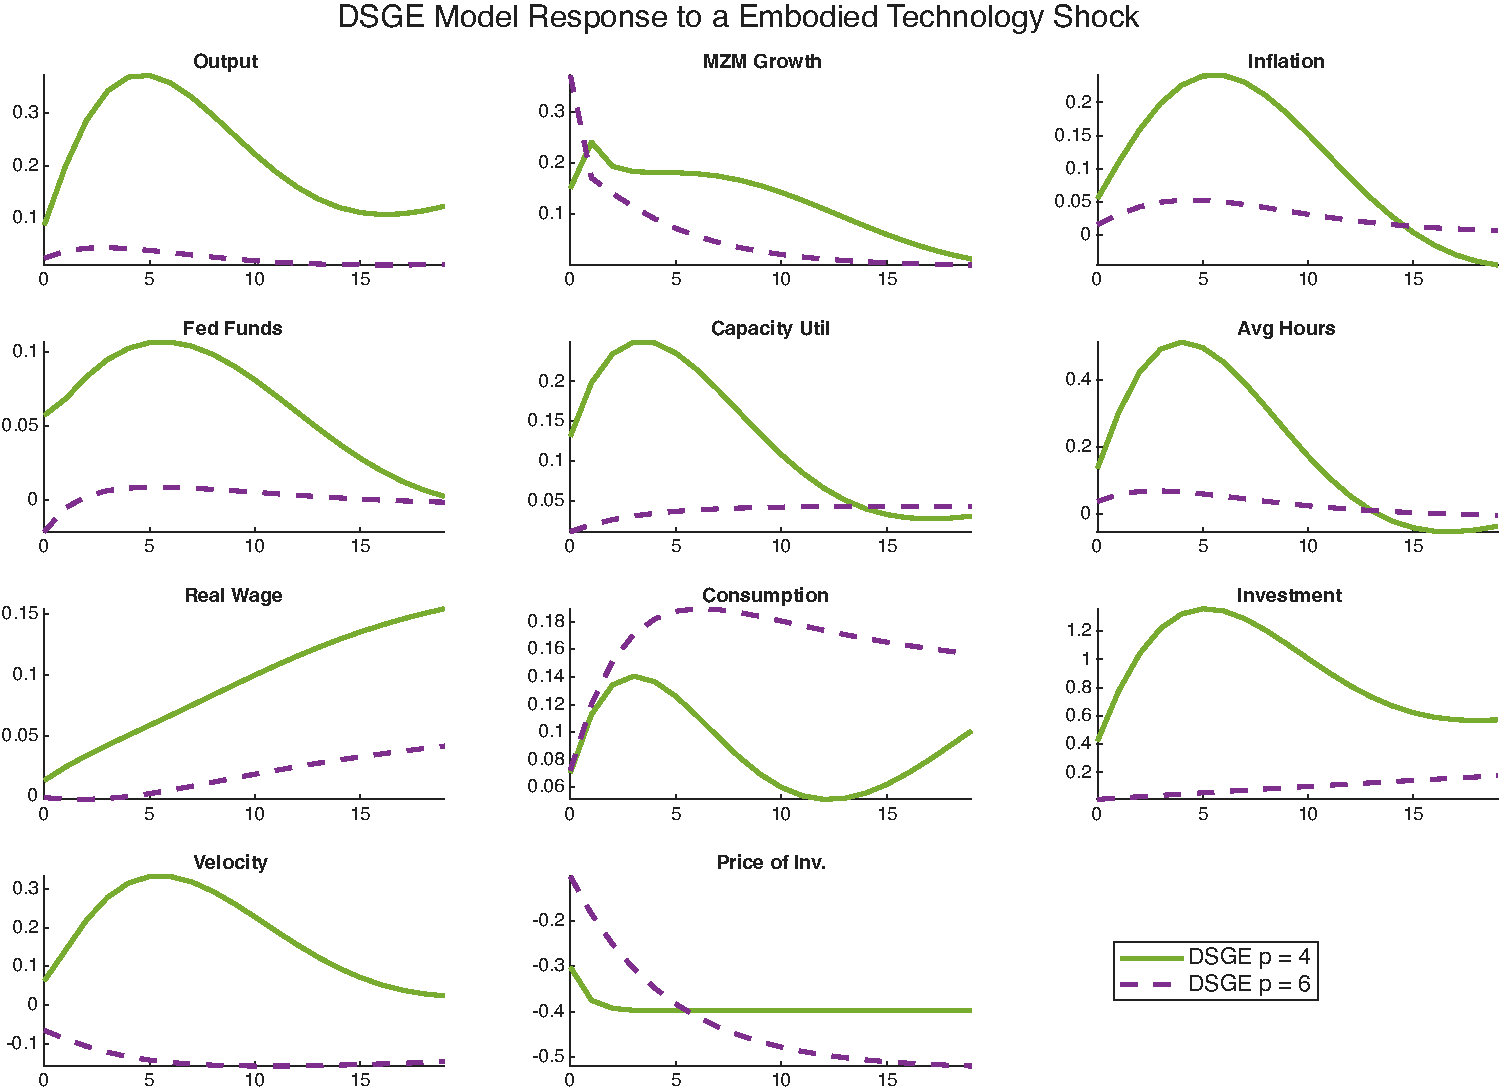
\includegraphics[width=1\linewidth]{../../Output/DSGE_IRFs_Long_Lag_Progressively_Plots/Embodied_Technology_Shock/Step_2_UpToLag_6.pdf}}{\fbox{Image Path Broken or File Missing}}
    \caption{DSGE Embodied Technology Shock lag 6}
    \label{fig:DSGE_et_baseline_lag6}
\end{figure}

\begin{figure}[htpb]
    \centering
    \IfFileExists{../../Output/DSGE_IRFs_Long_Lag_Progressively_Plots/Embodied_Technology_Shock/Step_3_UpToLag_8.pdf}
    {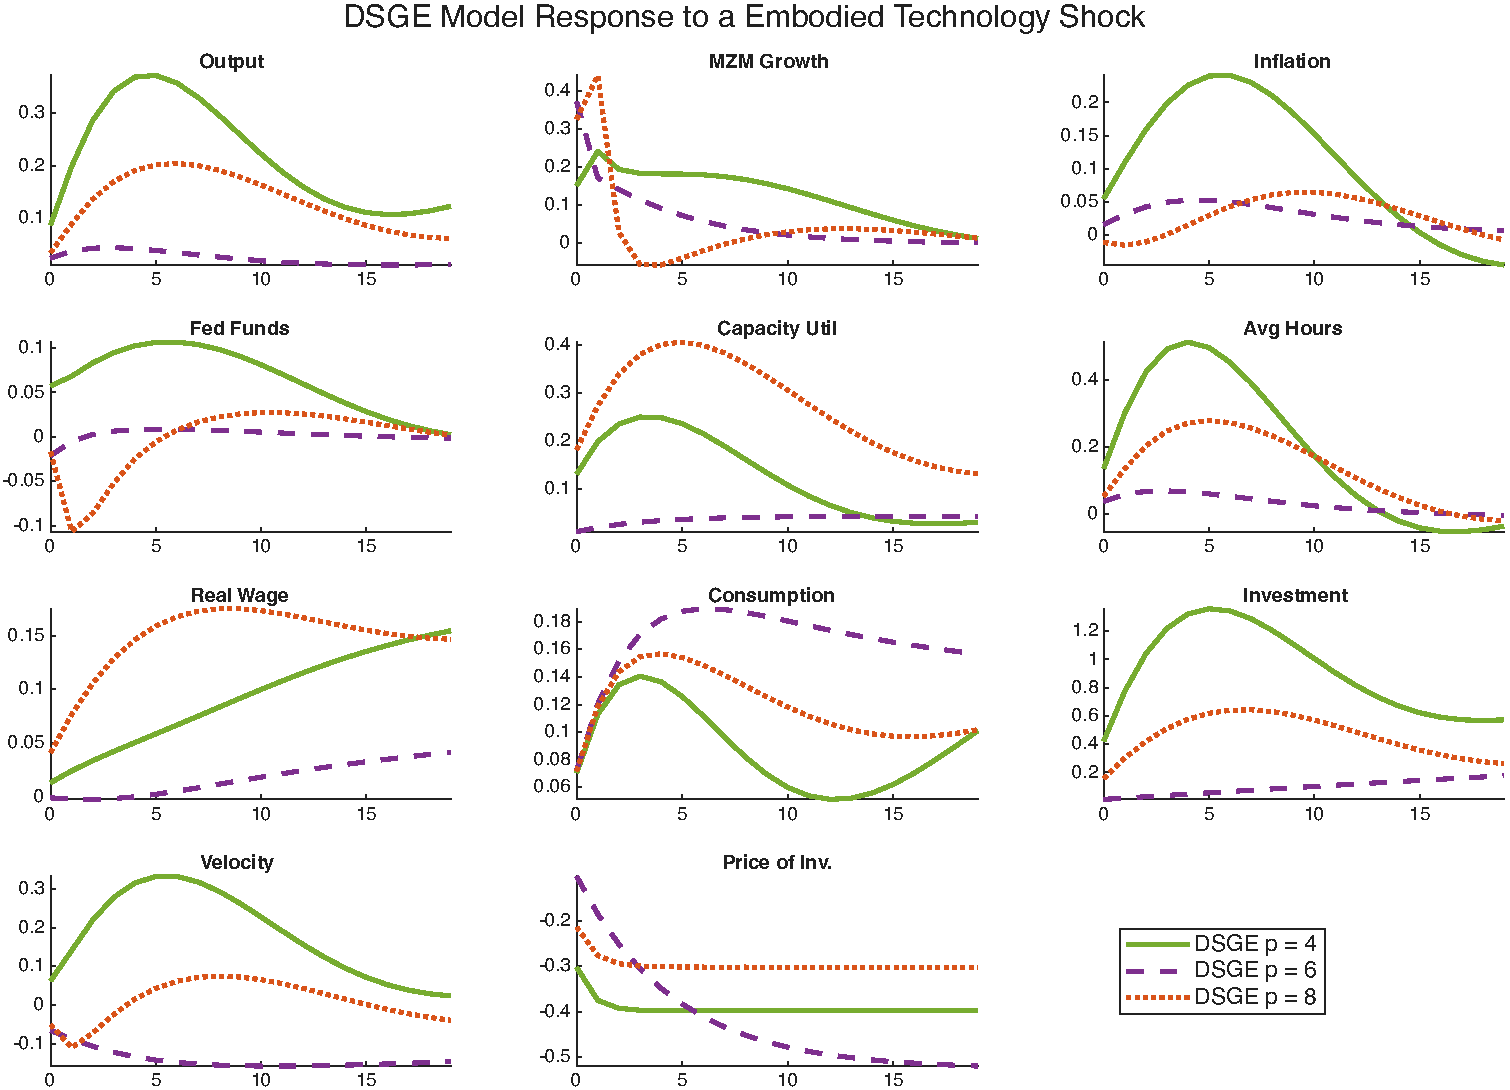
\includegraphics[width=1\linewidth]{../../Output/DSGE_IRFs_Long_Lag_Progressively_Plots/Embodied_Technology_Shock/Step_3_UpToLag_8.pdf}}{\fbox{Image Path Broken or File Missing}}
    \caption{DSGE Embodied Technology Shock lag 8}
    \label{fig:DSGE_et_baseline_lag8}
\end{figure}

\begin{figure}[htpb]
    \centering
    \IfFileExists{../../Output/DSGE_IRFs_Long_Lag_Progressively_Plots/Embodied_Technology_Shock/Step_4_UpToLag_10.pdf}
    {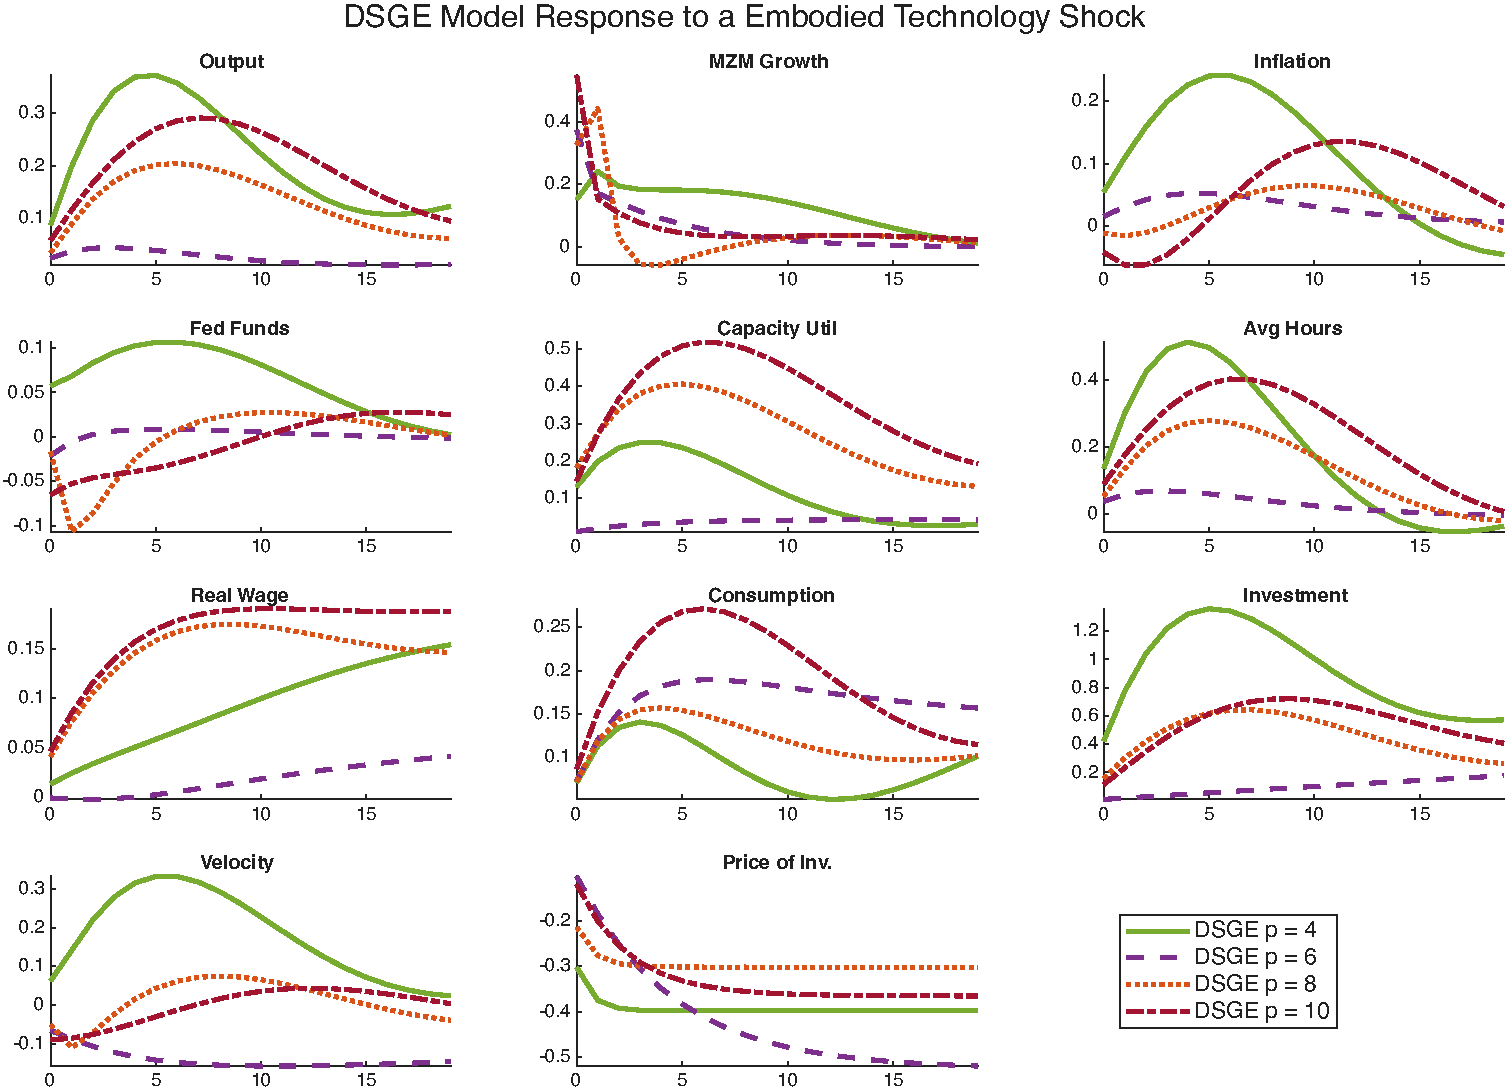
\includegraphics[width=1\linewidth]{../../Output/DSGE_IRFs_Long_Lag_Progressively_Plots/Embodied_Technology_Shock/Step_4_UpToLag_10.pdf}}{\fbox{Image Path Broken or File Missing}}
    \caption{DSGE Embodied Technology Shock lag 10}
    \label{fig:DSGE_et_baseline_lag10}
\end{figure}

\begin{figure}[htpb]
    \centering
    \IfFileExists{../../Output/DSGE_IRFs_Long_Lag_Progressively_Plots/Embodied_Technology_Shock/Step_5_UpToLag_12.pdf}
    {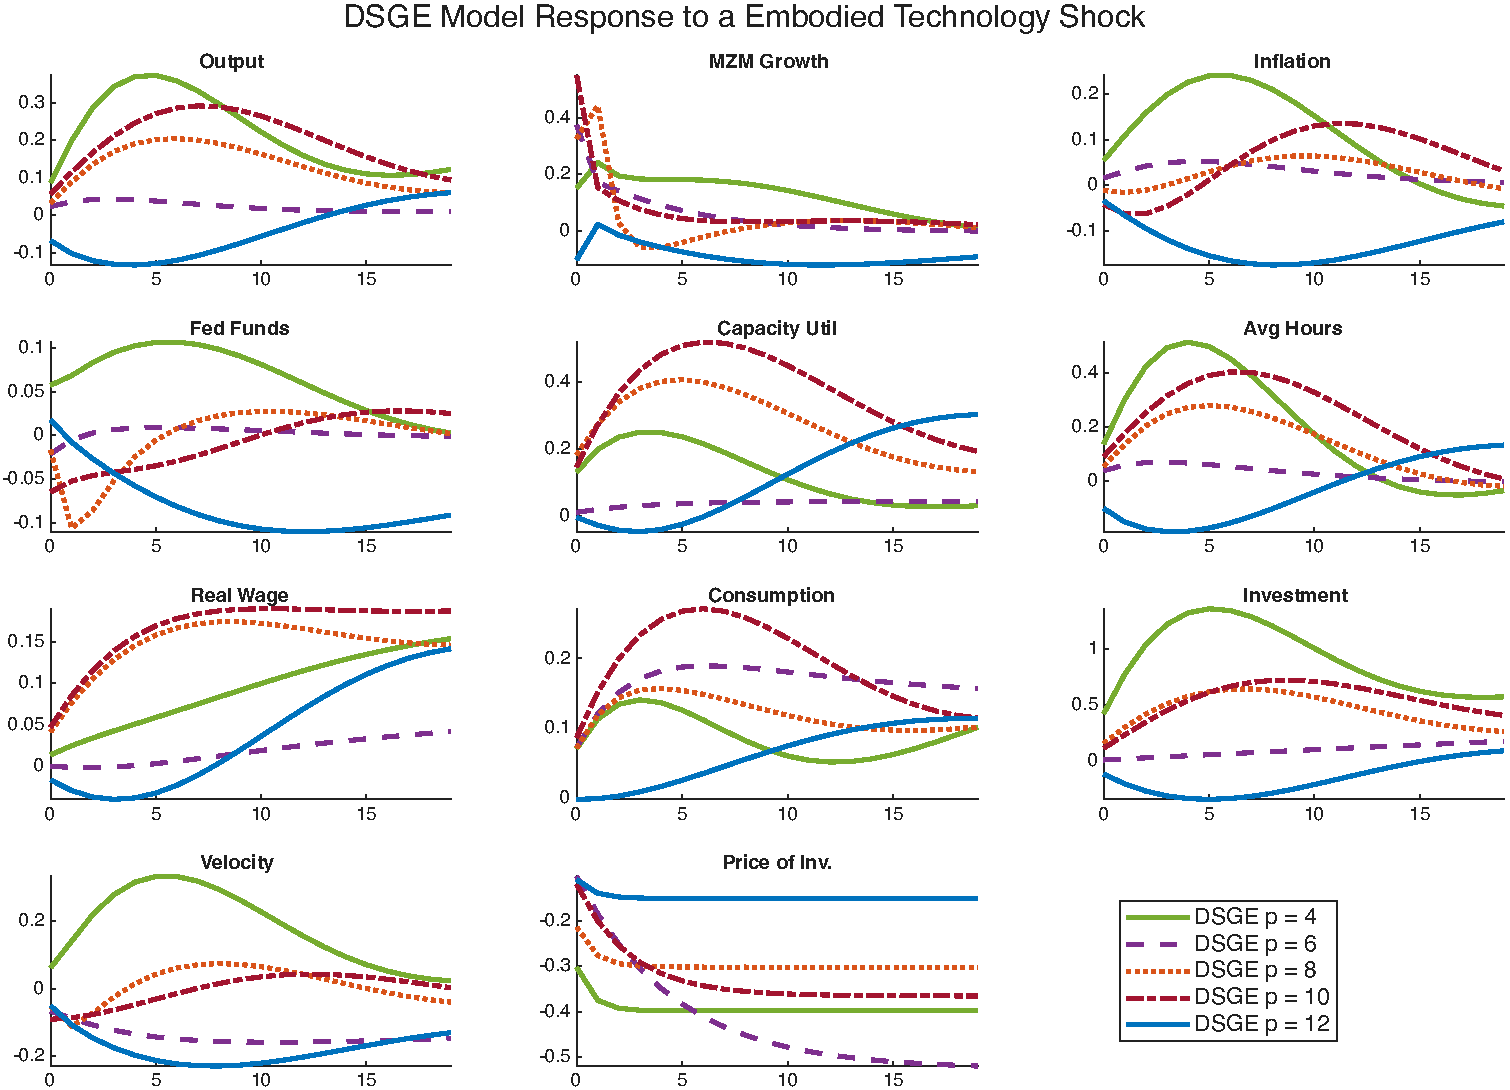
\includegraphics[width=1\linewidth]{../../Output/DSGE_IRFs_Long_Lag_Progressively_Plots/Embodied_Technology_Shock/Step_5_UpToLag_12.pdf}}{\fbox{Image Path Broken or File Missing}}
    \caption{DSGE Embodied Technology Shock lag 12}
    \label{fig:DSGE_et_baseline_lag12}
\end{figure}

\FloatBarrier
\subsection{ACEL 2005 DSGE Across different lag structures Progressively Comparison: Neutral Technology Shock}

\begin{figure}[htpb]
    \centering
    \IfFileExists{../../Output/DSGE_IRFs_Long_Lag_Progressively_Plots/Neutral_Technology_Shock/Step_1_UpToLag_4.pdf}
    {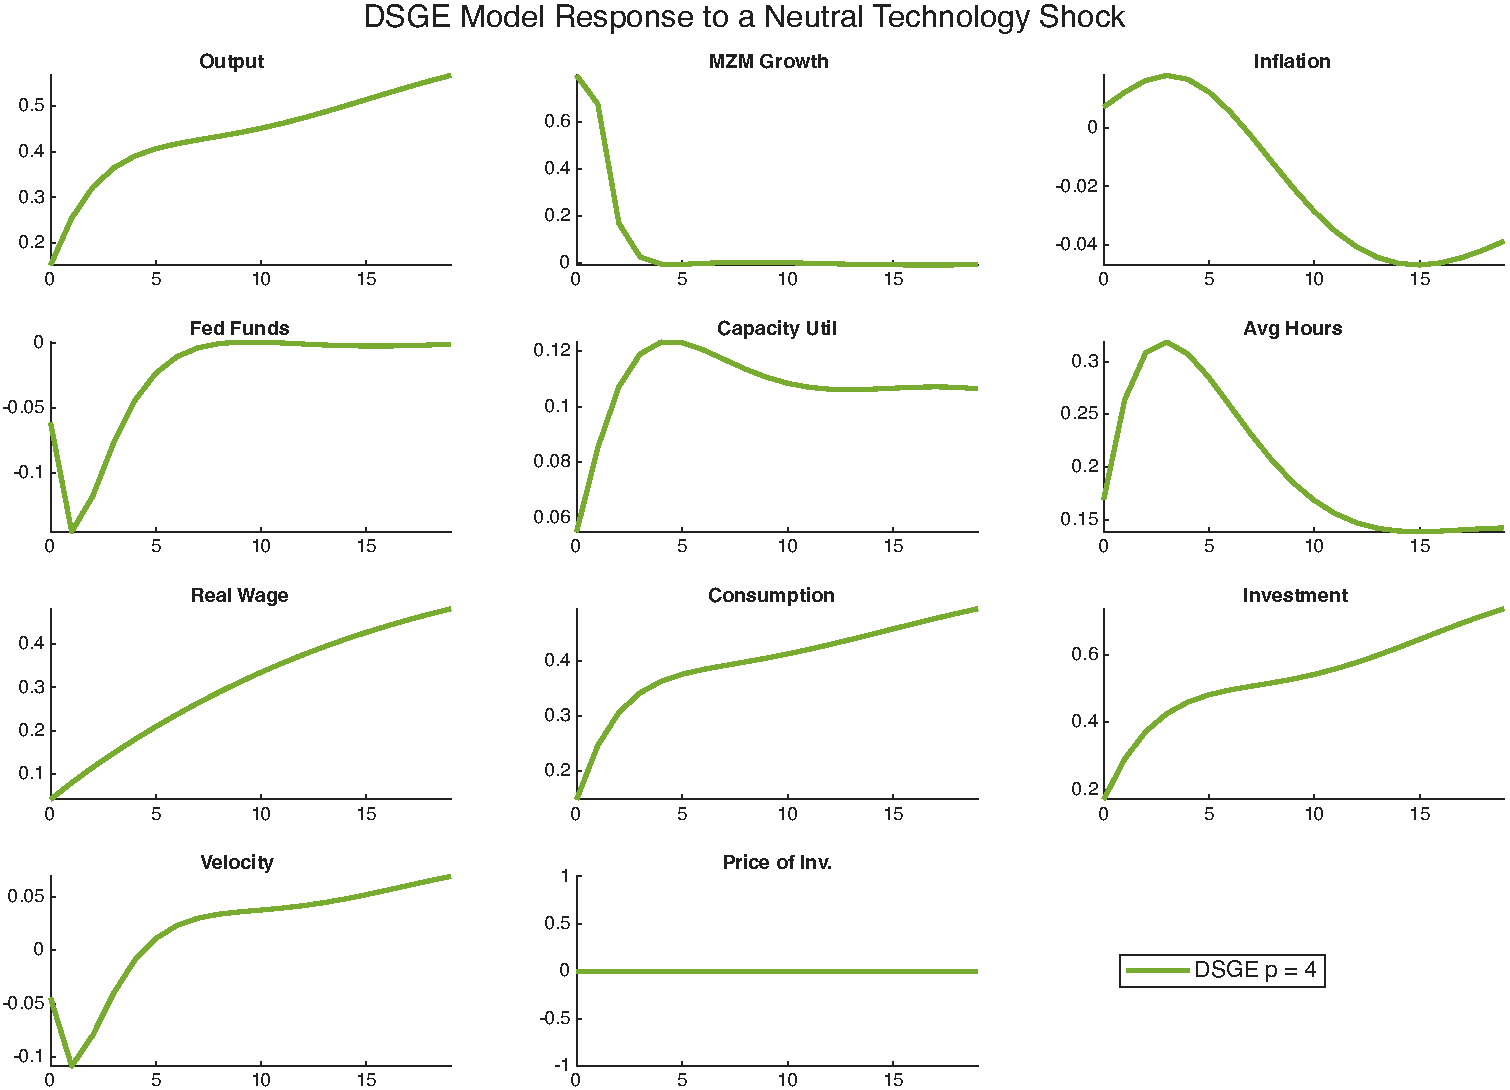
\includegraphics[width=1\linewidth]{../../Output/DSGE_IRFs_Long_Lag_Progressively_Plots/Neutral_Technology_Shock/Step_1_UpToLag_4.pdf}}{\fbox{Image Path Broken or File Missing}}
    \caption{DSGE Neutral Technology Shock lag 4}
    \label{fig:DSGE_nt_baseline_lag4}
\end{figure}

\begin{figure}[htpb]
    \centering
    \IfFileExists{../../Output/DSGE_IRFs_Long_Lag_Progressively_Plots/Neutral_Technology_Shock/Step_2_UpToLag_6.pdf}
    {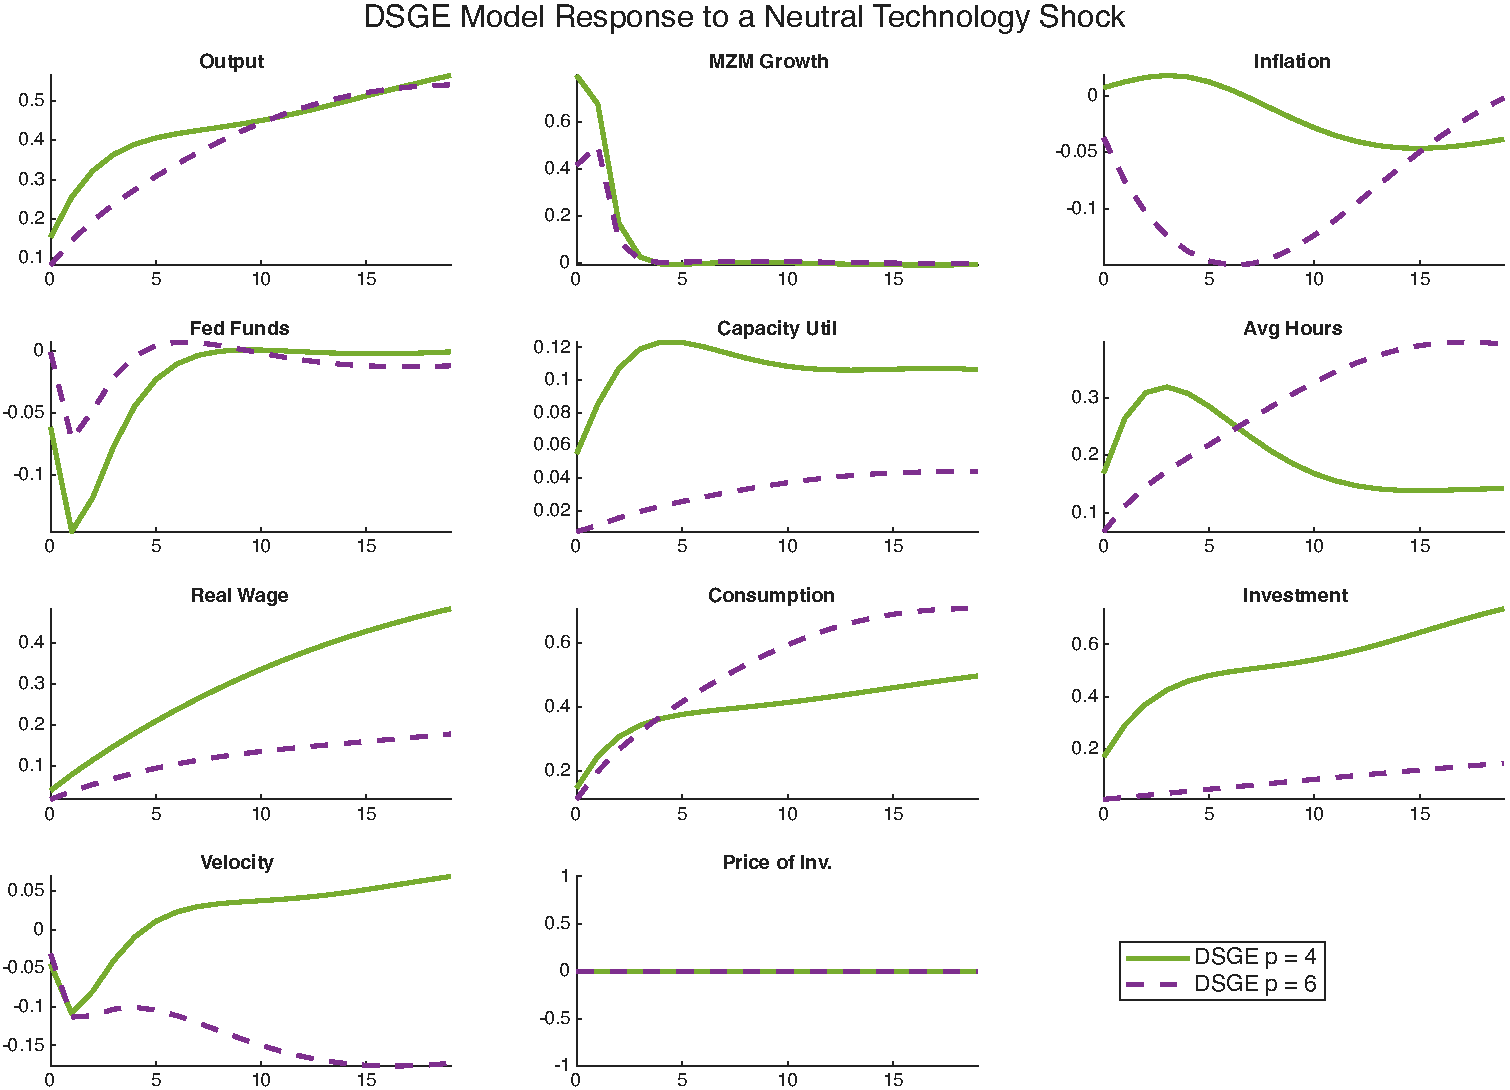
\includegraphics[width=1\linewidth]{../../Output/DSGE_IRFs_Long_Lag_Progressively_Plots/Neutral_Technology_Shock/Step_2_UpToLag_6.pdf}}{\fbox{Image Path Broken or File Missing}}
    \caption{DSGE Neutral Technology Shock lag 6}
    \label{fig:DSGE_nt_baseline_lag6}
\end{figure}

\begin{figure}[htpb]
    \centering
    \IfFileExists{../../Output/DSGE_IRFs_Long_Lag_Progressively_Plots/Neutral_Technology_Shock/Step_3_UpToLag_8.pdf}
    {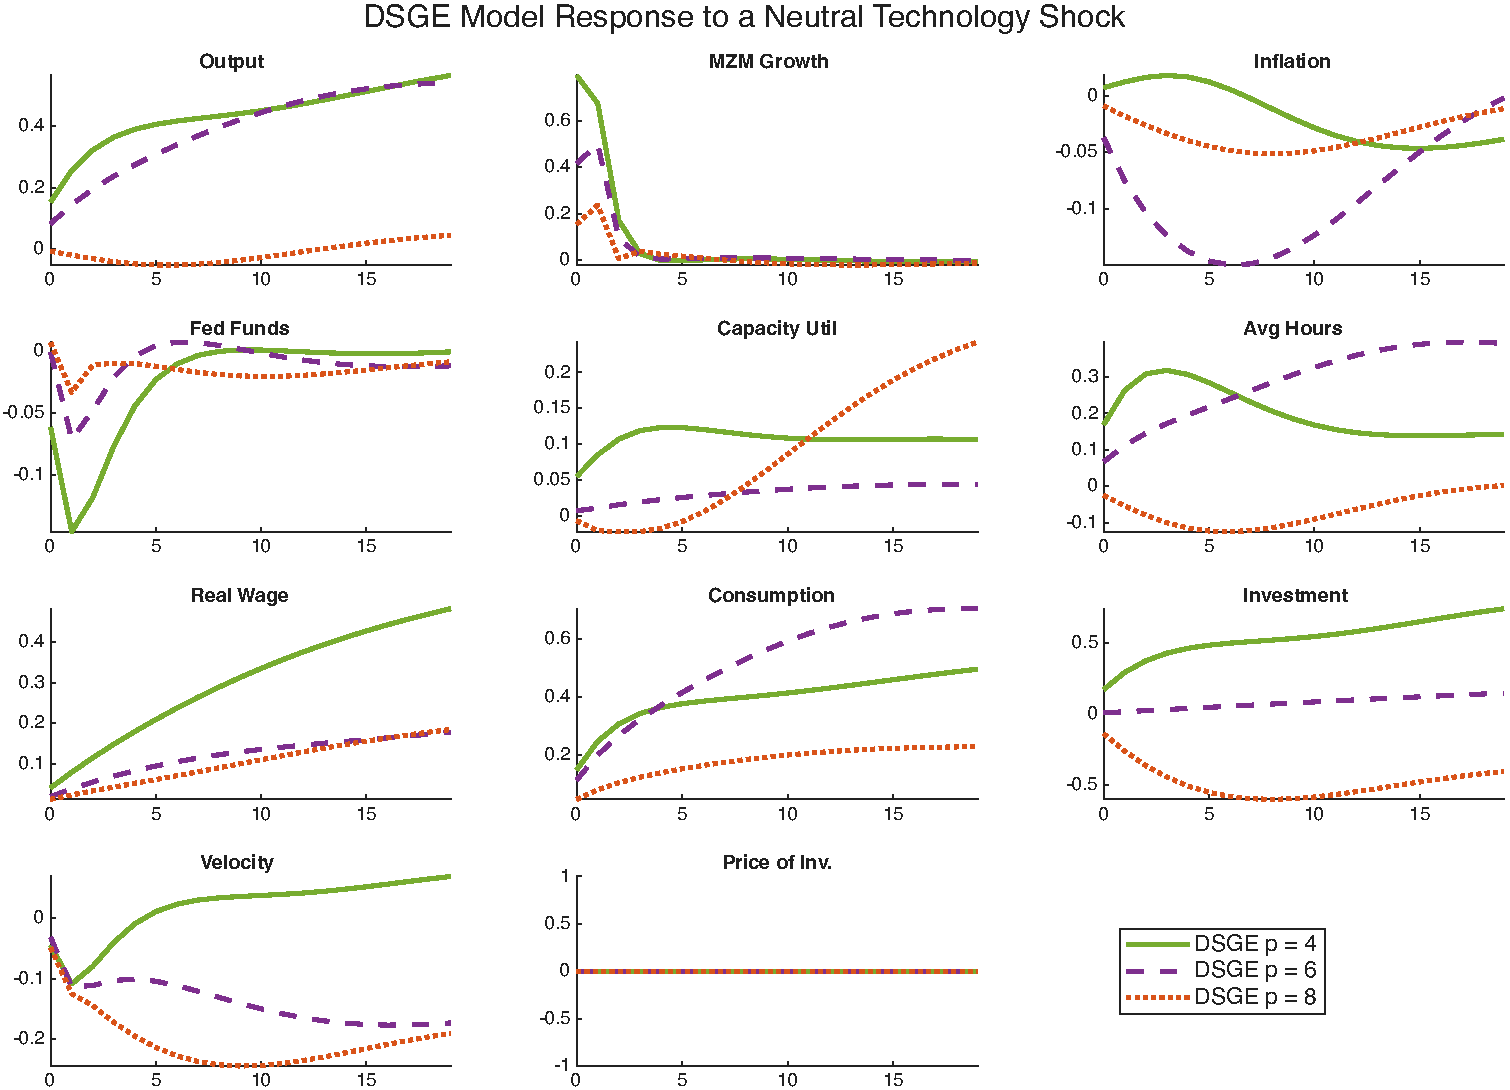
\includegraphics[width=1\linewidth]{../../Output/DSGE_IRFs_Long_Lag_Progressively_Plots/Neutral_Technology_Shock/Step_3_UpToLag_8.pdf}}{\fbox{Image Path Broken or File Missing}}
    \caption{DSGE Neutral Technology Shock lag 8}
    \label{fig:DSGE_nt_baseline_lag8}
\end{figure}

\begin{figure}[htpb]
    \centering
    \IfFileExists{../../Output/DSGE_IRFs_Long_Lag_Progressively_Plots/Neutral_Technology_Shock/Step_4_UpToLag_10.pdf}
    {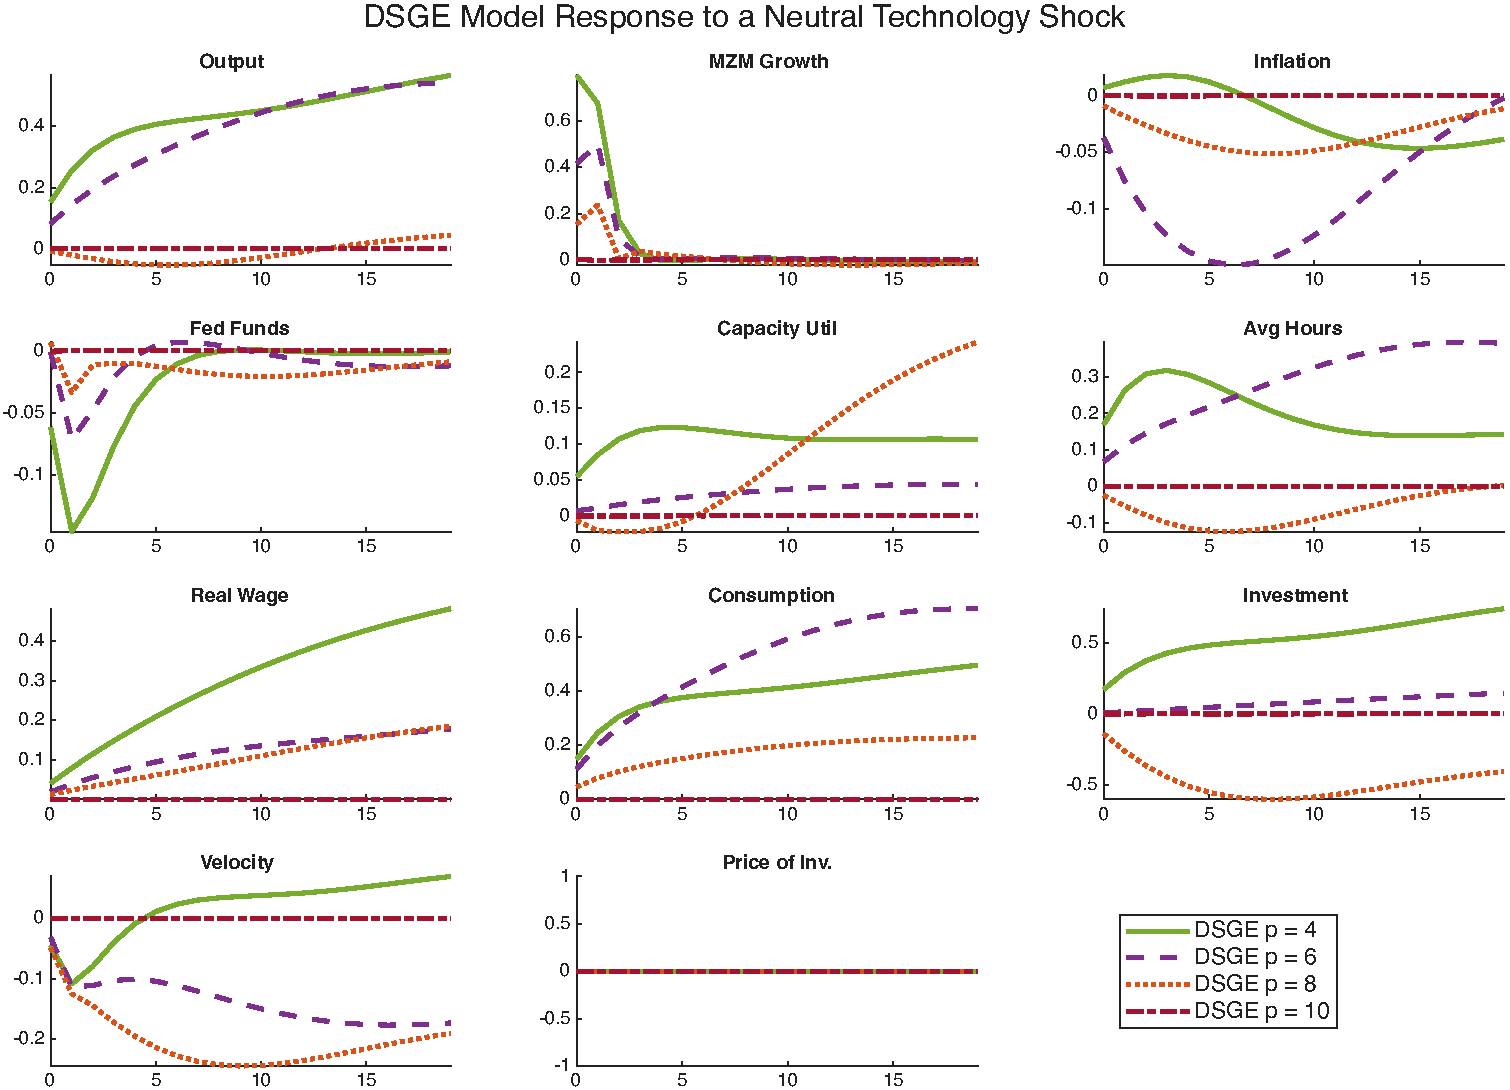
\includegraphics[width=1\linewidth]{../../Output/DSGE_IRFs_Long_Lag_Progressively_Plots/Neutral_Technology_Shock/Step_4_UpToLag_10.pdf}}{\fbox{Image Path Broken or File Missing}}
    \caption{DSGE Neutral Technology Shock lag 10}
    \label{fig:DSGE_nt_baseline_lag10}
\end{figure}

\begin{figure}[htpb]
    \centering
    \IfFileExists{../../Output/DSGE_IRFs_Long_Lag_Progressively_Plots/Neutral_Technology_Shock/Step_5_UpToLag_12.pdf}
    {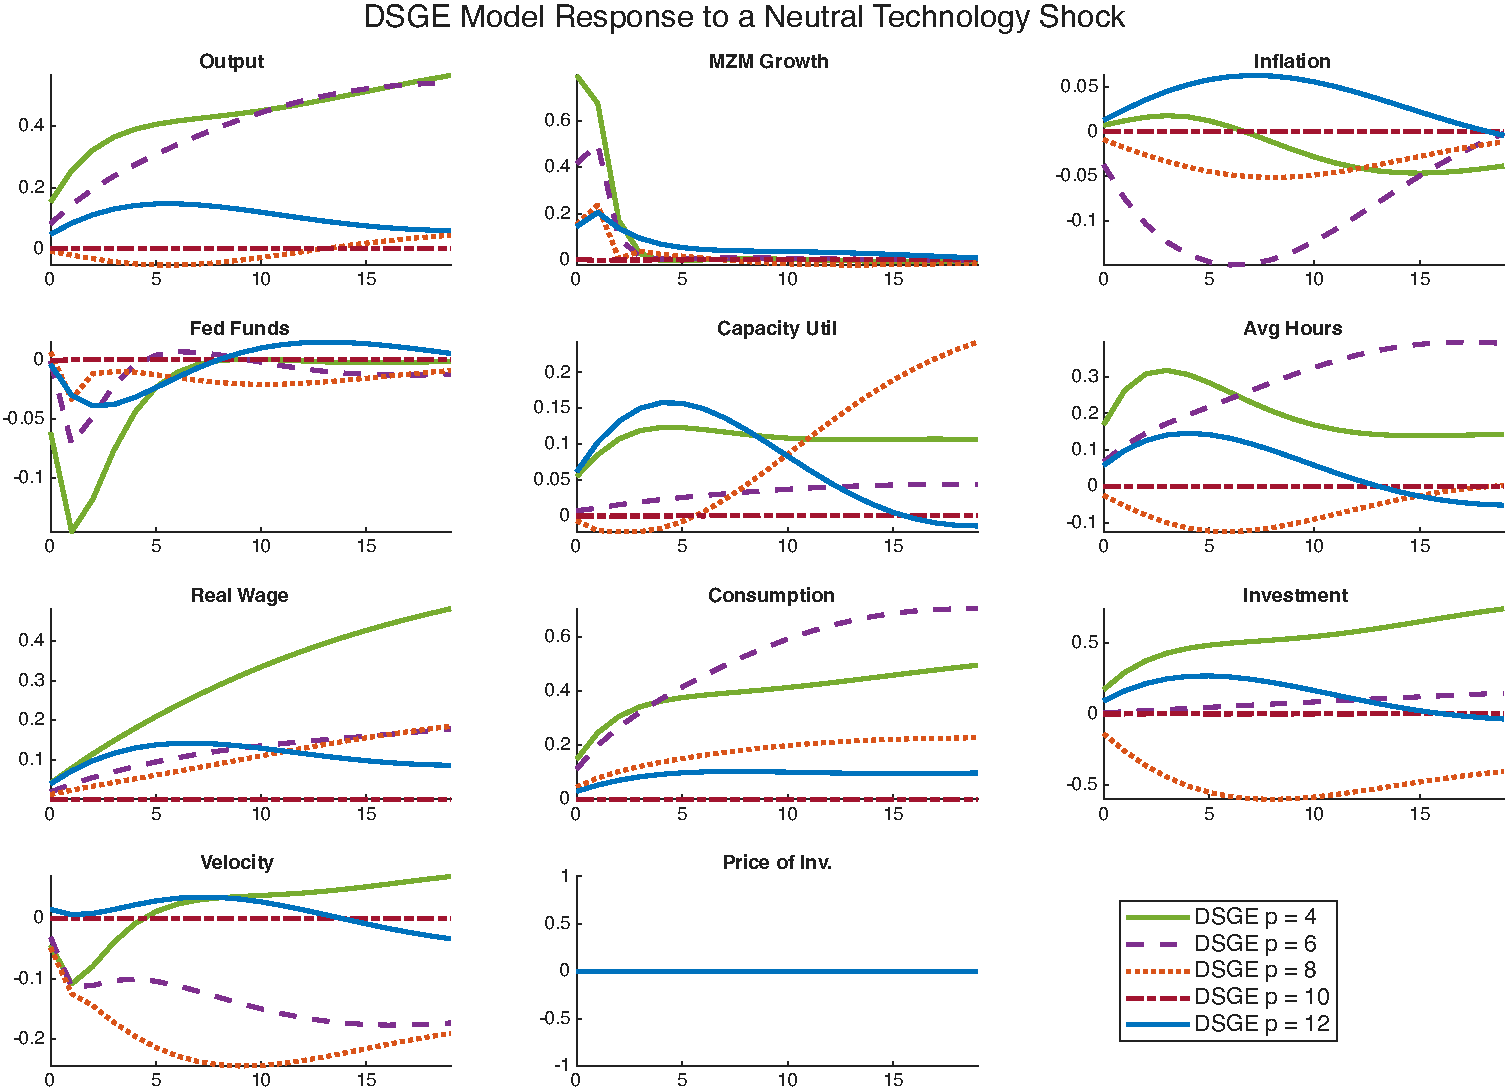
\includegraphics[width=1\linewidth]{../../Output/DSGE_IRFs_Long_Lag_Progressively_Plots/Neutral_Technology_Shock/Step_5_UpToLag_12.pdf}}{\fbox{Image Path Broken or File Missing}}
    \caption{DSGE Neutral Technology Shock lag 12}
    \label{fig:DSGE_nt_baseline_lag12}
\end{figure}

\FloatBarrier

\end{document}